\documentclass{report}
\usepackage{amsthm,amsmath,amssymb,braket,multirow,caption,relsize,tocbibind,color,appendix,enumitem,cite,graphicx}
\usepackage[hidelinks]{hyperref}
\usepackage[margin=0.7in,bottom=1in]{geometry}

\setcounter{tocdepth}{1}
\numberwithin{equation}{section}
\allowdisplaybreaks
\bibliographystyle{unsrt}

\title{\bf A Unitary RG-based Auxiliary Model Approach to Strongly-Correlated Electronic Systems}
\author{Abhirup Mukherjee, N.S. Vidhyadhiraja, A. Taraphder, Siddhartha Lal}
\date{\today}

\begin{document}
\maketitle
\tableofcontents
\newpage
\chapter{Introduction}

\section{What is the minimal impurity model for a Mott metal-insulator transition?}
\label{sec:min_model}
The Hubbard model is one of the fundamental models for strong electronic correlation; in its simplest form, it features a single band of conduction electrons hopping on a lattice and interacting via local correlations that provide a cost \(U\) if any site is doubly occupied:
\[H_\text{hubb} = -t\sum_{\left<i,j \right>,\sigma}\left(c^\dagger_{i\sigma}c_{j\sigma}+\text{h.c.}\right) + U\sum_i \hat n_{i \uparrow} \hat n_{i \downarrow} - \mu \sum_{i,\sigma}\hat n_{i\sigma}\]
The model can be made particle-hole symmetric by choosing \(\mu = U/2\):
\[H_\text{hubb} = -t\sum_{\left<i,j \right>,\sigma}\left(c^\dagger_{i\sigma}c_{j\sigma}+\text{h.c.}\right) - \frac{U}{2}\sum_i \left(\hat n_{i \uparrow} - \hat n_{i \downarrow}\right)^2\]
There are two trivial limits of the model. At \(U=0\), the bath consists of just a kinetic energy part, and the ground state is just a filled Fermi sea. At \(t=0\), each lattice site decouples from the rest and becomes a local moment, which under symmetry-breaking becomes a Néel antiferromagnet. This suggests that on increasing \(U/t\) beyond some critical value, the system might undergo a phase transition from a metallic state to an insulating state~\cite{Mott_1949}. This transition is reflected in the local spectral function - while it has a well-defined zero energy peak in the metallic phase, it is gapped in the insulating phase.

One method of studying Hubbard models is through auxiliary models, described in the next section. Auxiliary models are simpler versions of the full Hamiltonian that are able to capture the essential physics. For example, a correlated impurity interacting with a conduction bath is a potential auxiliary model for the Hubbard Hamiltonian:
\begin{equation}
\label{clus_bath_siam}
\mathcal{H}_\text{SIAM} = \epsilon_d \hat n_d + U \hat n_{d \uparrow} \hat n_{d \downarrow} - t\sum_{\left<i,j \right>, \sigma}\left(c^\dagger_{i\sigma}c_{j\sigma} + \text{h.c.}\right) + V\sum_\sigma \left( c^\dagger_{d\sigma}c_{0\sigma} + \text{h.c.}\right) 
\end{equation}
The impurity has onsite energy \(\epsilon_d\) and an onsite correlation \(U\). It hybridises into the bath through \(V\).

If the impurity site hybridises with a {\it non-interacting} bath defined by a uniform density of states, the impurity spectral function is found to have a well-defined Kondo resonance at low temperatures. Increasing the impurity correlation \(U\) only serves to reduce the width of the central peak at the cost of the appearance of side bands at energy scales of the order of \(U\), but the resonance never dies. The situation is however different if the impurity is embedded in a correlated conduction bath with a non-trivial density of states. For the case of a conduction band with the DOS shown in the right of the figure below, the impurity hybridises into a reduced bandwidth because of the correlation on the lattice~\cite{held_2013}.

This difference in the type of conduction baths is utilised in dynamical mean-field theory to describe various phases of the bulk system.
This is done through the DMFT algorithm: one starts with a non-interacting bath, but depending on the value of \(U\), the conduction bath then gets modified and we ultimately end up with something that is different from what we started with.
For small \(U\), the bath does not change much and we retain the central resonance of the impurity spectral function.
This then describes a metal in the bulk.
For larger values of \(U\), however, the bath changes significantly such that its density of states becomes non-constant.
Above a critical \(U_c\), the impurity spectral function gets gapped out, and that then describes the insulating phase in the bulk.
\textit{This leaves open the following question: What is the minimal correlation one can insert into the non-interacting bath (of a single-impurity Anderson model) that can capture both the metallic and insulating phases of the bulk model?}

\begin{figure}[!htb]
\centering
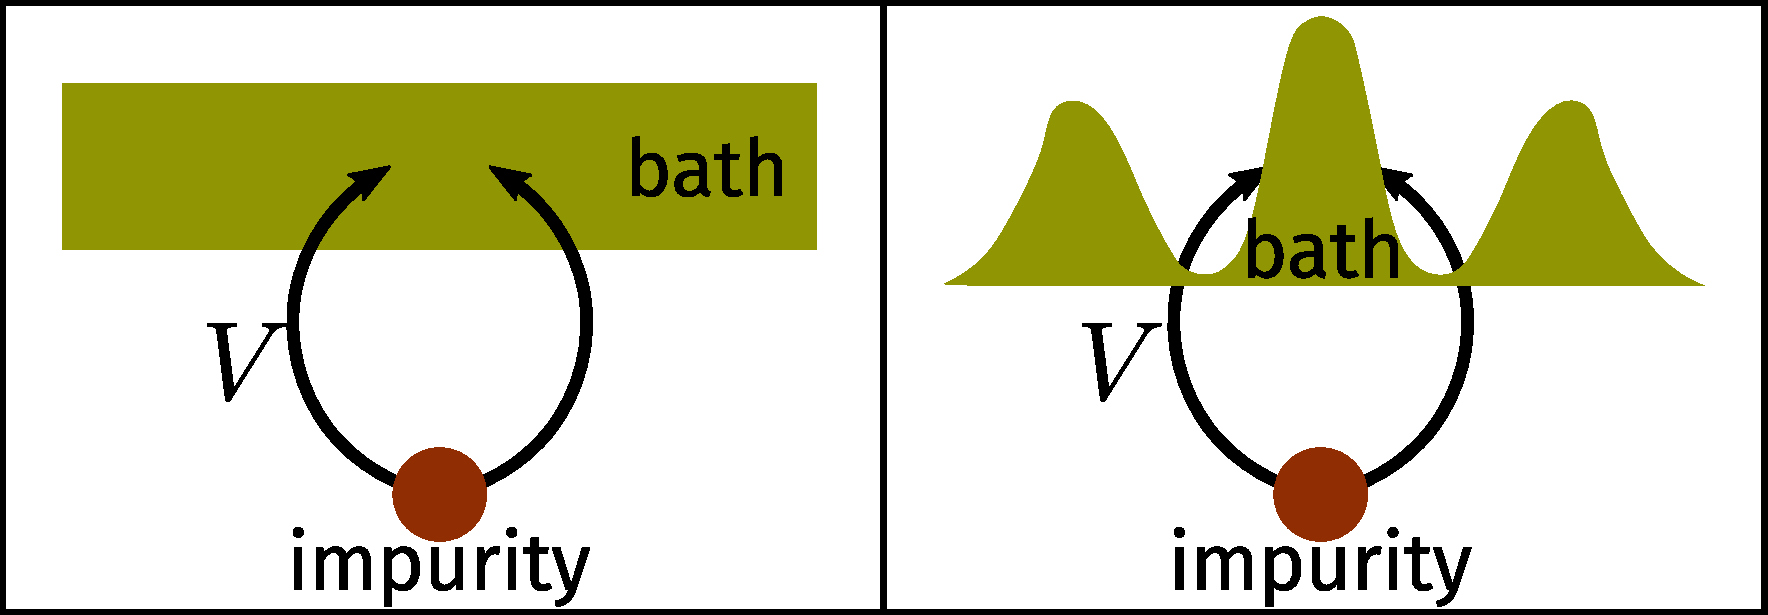
\includegraphics[width=0.5\textwidth]{dos_diff.pdf}
\caption{Various kinds of bath that an impurity can hybridise into. The left panel shows a non-interacting conduction band with a flat density of states. The right panel shows an interacting bath with an energy-dependent density of states. In the latter case, the impurity "feels" a reduced effective bandwidth defined by the width of the central peak.}
\end{figure}

\section{Philosophy of auxiliary model methods}
The present method is a realisation of the general method of using simpler systems called auxiliary models to study bulk systems~\cite{martin_2016}. In general, a full Hamiltonian can be separated into the Hamiltonians for a particular subsystem \(S\), the rest of the system \(R\), and the interactions between \(S\) and \(R\).
\begin{equation}\begin{aligned}
	\mathcal{H} = \mathcal{H}_S\ket{S}\bra{S} + \mathcal{H}_R \ket{R}\bra{R} + \mathcal{H}_{SR} \ket{S}\bra{R} + \mathcal{H}_{RS}\ket{S}\bra{R} = \begin{bmatrix} & \mathcal{H}_{R} && \mathcal{H}_{RS} & \\ & \mathcal{H}_{RS}^* && \mathcal{H}_{S} & \end{bmatrix}
\end{aligned}\end{equation}
where \(\ket{S}\) and \(\ket{R}\) actually represents sums over all basis kets of \(S\) and \(R\) respectively. As an example, we can split the Hubbard model Hamiltonian between a particular site \(i = p\) and the rest of the lattice as follows (fig.~\ref{cluster-bath}):
\begin{equation}\begin{aligned}
	H_\text{hubb} &= \overbrace{U^H\hat n_{p \uparrow} \hat n_{p \downarrow} - \mu^H \sum_\sigma \hat n_{p \sigma}}^{H_S} + \underbrace{U^H\sum_{i \neq p}\hat n_{i \uparrow} \hat n_{p \downarrow} - \mu^H \sum_{i \neq p, \sigma} \hat n_{i \sigma} -t^H\sum_{\sigma,\left<i,j \right>\atop{i \neq p \neq j}}\left(c^\dagger_{i\sigma} c_{j\sigma} + \text{h.c.}\right)}_{H_R}\\
		      & -\underbrace{t^H\sum_{\sigma,\atop{i \in \text{N.N. of }p}}\left(c^\dagger_{i\sigma} c_{p\sigma} + \text{h.c.}\right)}_{H_{SR} + H_{RS}}\\
\end{aligned}\end{equation}
The Greens function of the full Hamiltonian can also be split in a similar fashion:
\begin{equation}\begin{aligned}
	G(\omega) = \begin{bmatrix} G_S && G_{SR} \\ G_{RS} && G_R \end{bmatrix}
\end{aligned}\end{equation}
Each Greens function can be written in terms of the non-interacting counterpart and the self-energy through the Dyson equation: \(\Sigma_i = 1/G_{i,0} - 1/G_i\).

The subsystem \(S\) is usually taken to be the "cluster", and consequently, \(R\) represents the "bath".
The smaller system is typically chosen such that its eigenstates are known exactly.
Progress is then made by choosing a simpler version of \(H_R\) and a simpler form also for its coupling \(H_{RS}\) with the smaller system.
This combination of the cluster and the simpler bath is then called the \textit{auxiliary system}.
A typical auxiliary system for the Hubbard model would be the SIAM, where the impurity represents an arbitrary site \(p\) of the lattice, the bath represents the rest of the lattice sites and the hybridisation term between the impurity and the bath represents the coupling term \(H_{RS}\).
Such a construction is shown in fig.~\ref{cluster-bath}.
\begin{figure}[!htb]
	\centering
	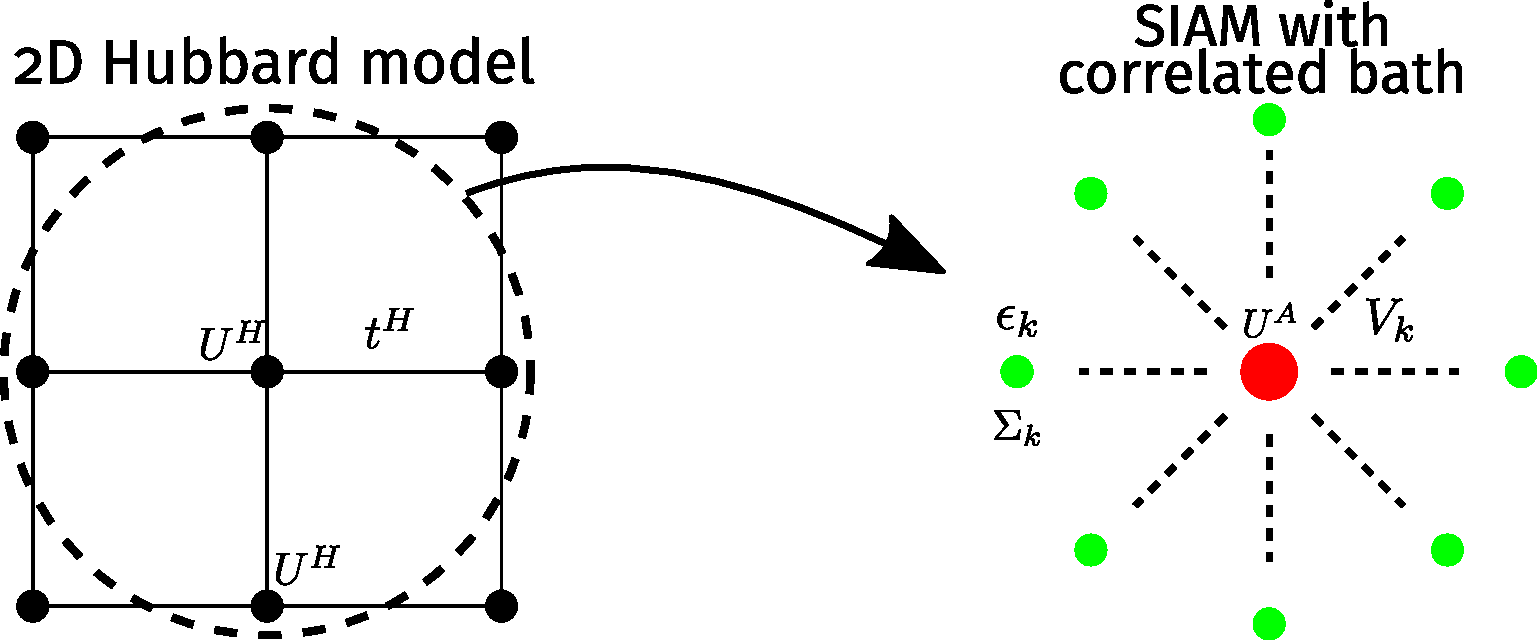
\includegraphics[width=0.8\textwidth]{cluster-bath.pdf}
	\caption{\textit{Left}: Full Hubbard model lattice with onsite repulsion $U^H$ on all sites and hopping between nearest neighbour sites with strength $t^H$. \textit{Right}: Extraction of the auxiliary (cluster+bath) system from the full lattice. The central site on left becomes the impurity site (red) on the right (with an onsite repulsion $\epsilon_d$), while the rest of the $N-1$ sites on the left form a conduction bath (green circles) (with dispersion $\epsilon_k$ and correlation modelled by the self-energy $\Sigma_k(\omega)$) that hybridizes with the impurity through the coupling $V$.}
	\label{cluster-bath}
\end{figure}
\textit{It should be noted that any reasonable choice of the cluster and bath would break the translational symmetry of the full model}. To allow computing quantities, one would need to make the bath (which is a much larger system) simpler than the cluster (which is a single site). This distinction breaks the translational symmetry of the Hubbard model. For eg., if one chooses eq.~\ref{clus_bath_siam} as the auxiliary system, then the fact that the impurity has an onsite correlation while the bath does not means we have broken the symmetry between the cluster and the bath.

\subsection*{Dynamical mean-field theory - an example of an auxiliary model approach}
Dynamical mean-field theory is an approximation scheme that use impurity models to obtain Greens functions of bulk systems of strong correlation~\cite{kotliar1996,kotliar1992}. The essential idea is to find the most suitable impurity model that replicates the full Hamiltonian. This is done through the following algorithm. Given a bulk Hamiltonian with on=site correlation \(U\) and a non-interacting \(k-\)space Greens function \(G_{k,0}\) for the bath:
\begin{itemize}
	\item[1.] We first create an impurity model with on-site correlation \(U\) and non-interacting impurity Greens function \(G_{i,0} = \sum_k G_{k,0}\).
		\[\mathcal{H}_\text{aux} = H_\text{imp}(U) -t \sum_\sigma \left(c^\dagger_{d\sigma}c_{0\sigma} + \text{h.c.}\right) + H_\text{bath}\left(t,G_{i,0}\right)\]

	\item[2.] This impurity model is solved using some method like numerical renormalisation group, and the self-energy \(\Sigma_\text{aux}\) of the impurity is obtained.

	\item[3.] The impurity self-energy is now {\it equated} with the bath momentum-space self-energy:
		\[\Sigma_{k}(\omega) = \Sigma_\text{aux}(\omega)\]
		Since the impurity is purely local, this is an approximation that involves replacing a non-local quantity by its purely local component: \(\Sigma_{k}(\omega) = \sum_{\vec r}e^{i \vec{k}\cdot\vec{r}}\Sigma_{\vec r}(\omega) \simeq \Sigma_{\vec r = 0}(\omega)\). This approximation is a result of the single-site nature of the cluster of the chosen auxiliary model - larger clusters with more impurities can generate non-local components. This local approximation becomes exact in the limit of large system dimension \(w\), because it can be shown that the non-local components of the self-energy scale as \(w^{-3/2}\).

	\item[4.] With this updated bath self-energy, we now create a new \(k-\)space Greens function for the bath:
		\[G_{i}(\omega) = \sum_k G_{k}(\omega) = \sum_k \frac{1}{\omega - H_\text{bath}(k) - \Sigma_k(\omega)} = \sum_k \frac{1}{\omega - H_\text{bath}(k) - \Sigma_\text{aux}(\omega)}\]
	This interacting Greens function is then used to obtain the updated non-interacting Greens function, using Dyson's equation:
	\[G_{i,0} = \frac{1}{1/G_{i} + \Sigma_\text{aux}}\]
	\item[5.] Repeat the algorithm from step 1 with the updated \(G_{i,0}\), until \(\Sigma_\text{aux}\) stops changing.
\end{itemize}
The stopping condition is the consistency relation that makes the bath and impurity self-energies equal.

\begin{figure}[!htb]
	\centering
	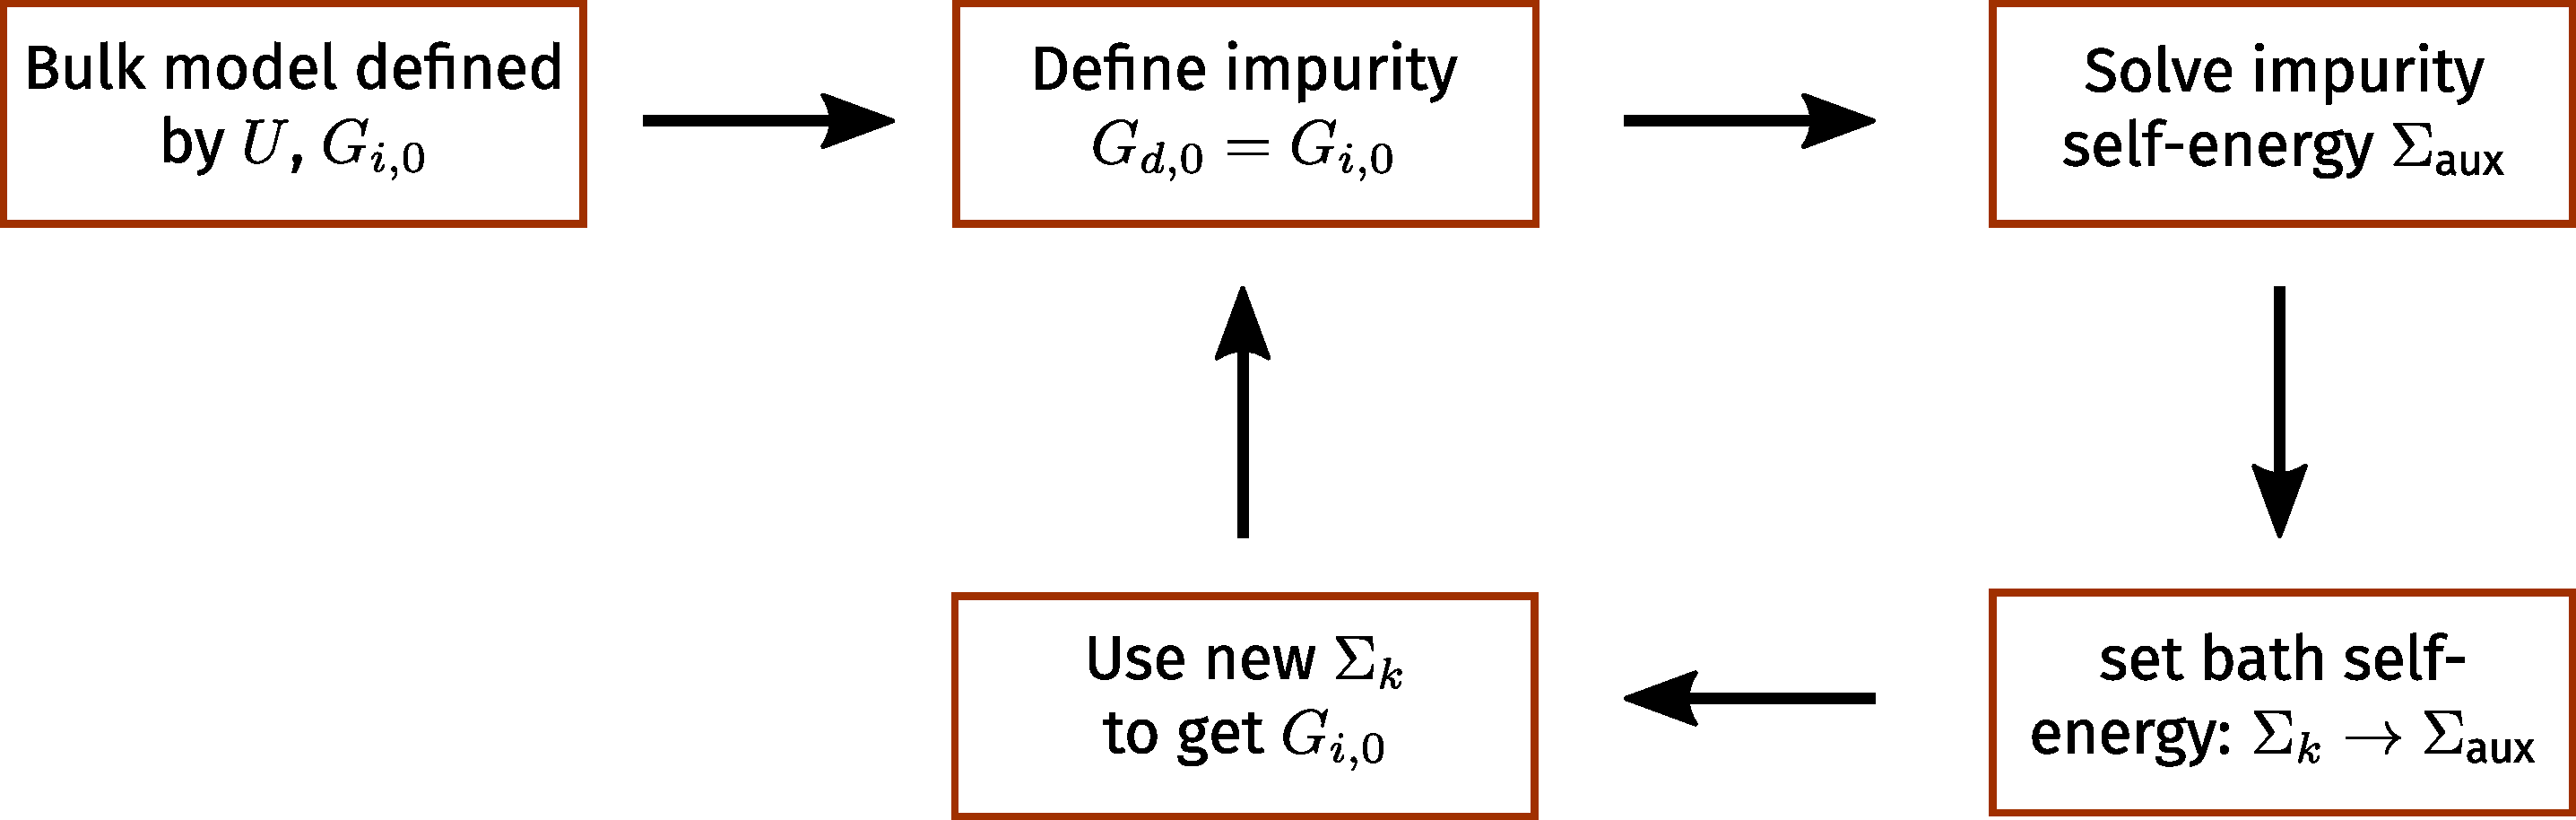
\includegraphics[width=0.8\textwidth]{dmft.pdf}
\end{figure}


\section{A ``bottoms-up" approach to using auxiliary models}
As mentioned in the previous section, the question we are posing is the following: what is the simplest auxiliary model of impurity in a bath that can capture the metal-insulator transition in a Hubbard-like model of correlated electrons. We approach this problem in a constructionist/bottoms-up way: we first identity an appropriate quantum impurity model (fig.~\ref{cluster-bath}) that shows an impurity phase transition, and then create a bulk model out of this auxiliary model. The bulk model hence created will then show a metal-insulator transition. The impurity models are studied using the recently-developed unitary renormalisation group method~\cite{anirbanmott1,anirbanmott2,anirbanurg1,anirbanurg2,siddharthacpi,santanukagome}. The leap to the bulk model is then made by applying lattice translation operators on the auxiliary model. This process is shown in chapter~\ref{chap:tile}. This process, referred to as tiling here, relates the auxiliary model Hamiltonian with that of the bulk, and hence allows connecting the Greens functions and other related quantities across dimensions. One nice outcome is that since the auxiliary model has multiple sites, there is a real-space off-diagonal component of the self-energy, and this leads to a \(k-\)dependence in the self-energy of the bulk, which is in contrast with the lack of \(k-\)dependence in single-site DMFT.  

In our approach, the auxiliary models can be chosen in various ways. The simplest choice is of course the single-impurity Anderson model of eq.~\ref{clus_bath_siam}:
\begin{equation}
\mathcal{H}_\text{SIAM} = \epsilon_d \hat n_d + U \hat n_{d \uparrow} \hat n_{d \downarrow} - t\sum_{\left<i,j \right>, \sigma}\left(c^\dagger_{i\sigma}c_{j\sigma} + \text{h.c.}\right) + V\sum_\sigma \left( c^\dagger_{d\sigma}c_{0\sigma} + \text{h.c.}\right) 
\end{equation}
This model does not show any impurity phase transition - the impurity is always screened~\cite{hrk_wilson_1980,wilson1975,bullaNRGreview}. Correlation can be introduced into the auxiliary model in two ways:
\begin{itemize}
	\item[1.] The impurity or the bath can be made to have additional interaction: 
\begin{gather}
\mathcal{H}_\text{aux} = H_\text{SIAM} + J \vec{S}_d\cdot\vec{s}_0 - \frac{1}{2}U_b \left(\hat n_{0 \uparrow} - \hat n_{0 \downarrow}\right)^2
\end{gather}
The additional terms are (i) a spin-exchange interaction between the impurity site and the zeroth site, and (ii) a local correlation on the zeroth site.
\item[2.] The second method is to make the cluster itself more complicated. That is, one can introduce multiple impurity sites that are connected via the hopping:
\begin{equation}
\mathcal{H}_\text{aux} = -\frac{U}{2}\sum_{d_i}\left(\hat n_{d_i \uparrow} - \hat n_{d_i \downarrow}\right) ^2 + V\sum_{d_i}\sum_\sigma\left( c^\dagger_{d_i\sigma}c_{0\sigma} + \text{h.c.} \right) + \text{K.E.} - t\sum_{\sigma}\left(c^\dagger_{d_1\sigma}c_{d_2\sigma} + \text{h.c.}\right)
\end{equation}
	
\end{itemize}

\begin{figure}[!htb]
 	\centering
 	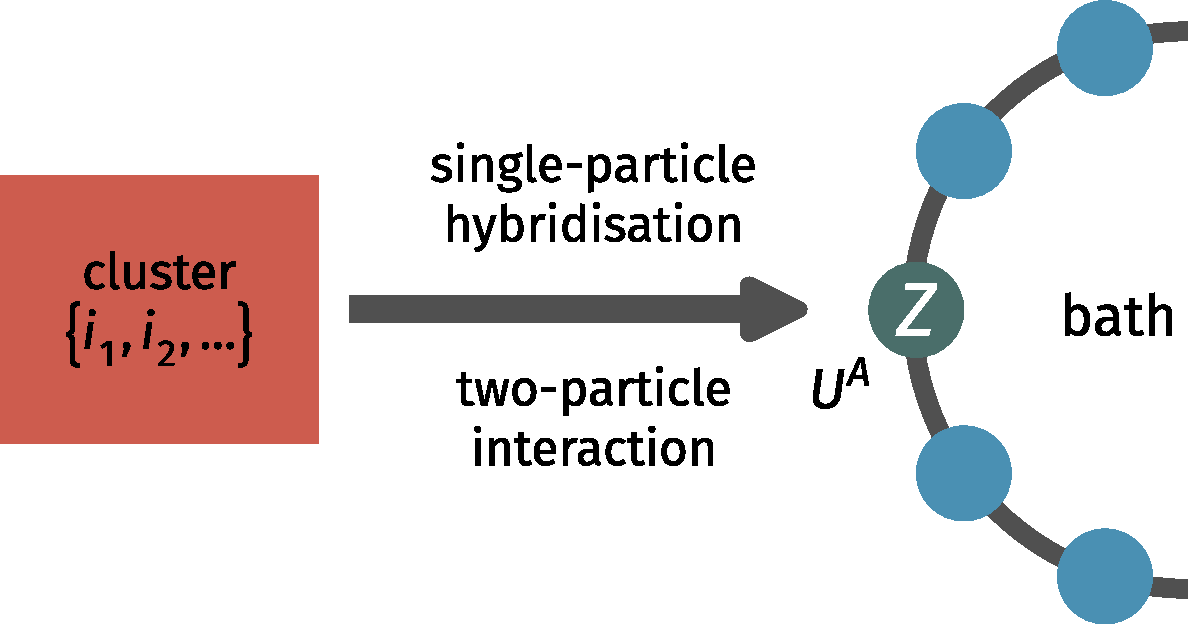
\includegraphics[width=0.6\textwidth]{gen_siam.pdf}
 	\caption{Cluster+bath construction of auxiliary model. It consists of a cluster (red square) hybridising with a bath (ring) by hopping into and out of the zeroth site (pink). The other sites (green) form the rest of the bath. Just the cluster and the zeroth site have onsite correlations.}
 \end{figure}
 The next step in the programme is to tile the real-space lattice with this cluster+bath Hamiltonian \(\tilde H\) to restore translational invariance (shown in a later section), and obtain a new bulk Hamiltonian for correlated electrons, $\tilde H = T\left[ \mathcal{H}_\text{aux} \right] T^{-1}$, where $T$ denotes the operator that performs the set of iterative real-space translations, and enables the cluster-bath (auxiliary model) Hamiltonian to span the target real-space lattice. Given a general auxiliary model Hamiltonian \(\mathcal{H}_\text{aux}\), the result of tiling can be written very generally as
 \begin{equation}\begin{aligned}
	 \tilde H = \sum_{\left\{i_1,i_2,...\right\}} \mathcal{H}_\text{aux}\left(\left\{i_1,i_2,...\right\}\right)
 \end{aligned}\end{equation}
where \(\left\{i_1,i_2,...\right\}\) represents the indices for the members of the cluster. To reiterate, what that means is that we have placed the cluster+bath system at all lattice point sets \(\left\{i_1,i_2,...\right\}\) to reconstruct a new model of correlated electrons. The answer to how closely $\tilde H$ approximates a target model of correlated electrons lies in (i) the choice of the cluster-bath construction of the auxiliary model, and (ii) the accuracy of the URG procedure on the auxiliary model.

The strategy, therefore, is to relate Hamiltonians, wavefunctions and hence correlation functions of the bulk model to those of the auxiliary model. One can then substitute the information obtained from solutions of the auxiliary model, and thereby calculate quantities on the bulk lattice model.

\chapter{From the auxiliary model to the bulk - single site approach}
\label{chap:tile}

\section{Creating a Hubbard-Heisenberg Hamiltonian from an extended Anderson impurity model}

Previously, we have worked out the ground-state phases of a single-impurity model with an interacting bath:
\begin{equation}\begin{aligned}
	\label{siam_attr}
	\mathcal{H}_\text{aux} = \sum_{k\sigma}\epsilon_k \tau_{k\sigma} - \frac{U}{2}\left(\hat n_{d \uparrow} - \hat n_{d \downarrow} \right) ^2 + \sum_{k\sigma} \left(V_{k} c^\dagger_{k\sigma} c_{d\sigma} + h.c.\right) +J \vec{S_d}\cdot\vec{s} - \frac{1}{2}U_b\left(\hat n_{0 \uparrow} - \hat n_{0 \downarrow}\right)^2 
\end{aligned}\end{equation}
 
We will use this as the auxiliary model to study the Hubbard model. We do this by first recreating the Hubbard model upon tiling the lattice with instances of this auxiliary model Hamiltonian. Note that the impurity level is explicitly at half-filling, because the correlation term \(\left( \hat n_{d \uparrow} - \hat n_{d \downarrow} \right) ^2\) is symmetric under a particle-hole transformation \(\hat n_{d\sigma} \to 1 - \hat n_{d\sigma}\). Moreover, the conduction bath is also at half-filling, because we have set the chemical potential \(\mu\) to zero. These two ensure that the bulk model is also at half-filling. At the end of this section, we will also mention how the tiling works out in the presence of a non-zero filling.

To begin this procedure, we first create the unit of tiling - this is done by identifying the impurity as a particular site \(i\) of the lattice, and the bath coupled to the impurity as the set of remaining \(N-1\) sites in the lattice. We will also identity the zeroth site of the SIAM lattice as one of the nearest neighbours \(j\) of \(i\):
\begin{equation}\begin{aligned}
	\mathcal{H}_\text{aux}(i,j) = -2t\sum_{<m,n>,\sigma}^{m \neq i \neq n} \left(c^\dagger_{m\sigma}c_{n\sigma} + \text{h.c.}\right) - \frac{U}{2}\left( \hat n_{i \uparrow} - \hat n_{i \downarrow} \right) ^2 + V \sum_{\sigma} \left(c^\dagger_{j\sigma} c_{i\sigma} + h.c.\right) +J \vec{S_i}\cdot\vec{S}_j - \frac{1}{2}U_b\left(\hat n_{j \uparrow} - \hat n_{j \downarrow}\right)^2 
\end{aligned}\end{equation}
The tight-binding term sums over all nearest pairs \((m,n)\) that do not involve the site \(i\).
In general \(i\) will have \(\mathcal{W}\) nearest neighbours for a lattice with coordination number \(\mathcal{W}\). The total local Hamiltonian for the site \(i\) is obtained by averaging over the Hamiltonians \(\mathcal{H}_\text{aux}(i,j)\) for all nearest neighbours \(j\) of \(i\):
\begin{equation}\begin{aligned}
	\mathcal{H}_\text{aux}(i) &= \frac{1}{\mathcal{W}}\sum_{j \in \text{NN of i}} \mathcal{H}_\text{aux}(i,j) = - \frac{U}{2}\left( \hat n_{i \uparrow} - \hat n_{i \downarrow} \right)^2 + \frac{1}{\mathcal{W}}\sum_{j \in \text{NN of i}}\left[-2t\sum_{<m,n>,\sigma}^{m \neq i \neq n}\left(c^\dagger_{m\sigma}c_{n\sigma} + \text{h.c.}\right) + V \sum_{\sigma} \left(c^\dagger_{j\sigma} c_{i\sigma} + h.c.\right)  \right.\\
				  &\left. +J \vec{S_i}\cdot\vec{S}_j - \frac{1}{2}U_b\left(\hat n_{j \uparrow} - \hat n_{j \downarrow}\right)^2\right]\\
				  &= - \frac{U}{2}\left( \hat n_{i \uparrow} - \hat n_{i \downarrow} \right)^2 -2t\sum_{<m,n>,\sigma}^{m \neq i \neq n}\left(c^\dagger_{m\sigma}c_{n\sigma} + \text{h.c.}\right) +  \frac{1}{\mathcal{W}}\sum_{j \in \text{NN of i}}\left[V \sum_{\sigma} \left(c^\dagger_{j\sigma} c_{i\sigma} + h.c.\right) +J \vec{S_i}\cdot\vec{S}_j \right.\\
				  &\left.- \frac{1}{2}U_b\left(\hat n_{j \uparrow} - \hat n_{j \downarrow}\right)^2\right]
\end{aligned}\end{equation}
Once we have this local Hamiltonian for a particular site, we translate this over all sites \(i\):
\begin{equation}\begin{aligned}
	\mathcal{H}_\text{full} =& \sum_i \mathcal{H}_\text{aux}(i) = \sum_i\left[- \frac{U}{2}\left( \hat n_{i \uparrow} - \hat n_{i \downarrow} \right)^2 -2t\sum_{<m,n>,\sigma}^{m \neq i \neq n}\left(c^\dagger_{m\sigma}c_{n\sigma} + \text{h.c.}\right) +  \frac{1}{\mathcal{W}}\sum_{j \in \text{NN of i}}\left[V \sum_{\sigma} \left(c^\dagger_{j\sigma} c_{i\sigma} + h.c.\right) \right.\right.\\
				  &\left.\left. + J \vec{S_i}\cdot\vec{S}_j - \frac{1}{2}U_b\left(\hat n_{j \uparrow} - \hat n_{j \downarrow}\right)^2\right]\right]\\
	=& -\frac{1}{2}\left(U + U_b\right) \sum_i \left( \hat n_{i \uparrow} - \hat n_{i \downarrow} \right)^2 + \sum_i\left[-2t\sum_{<m,n>,\sigma}^{m \neq i \neq n}\left(c^\dagger_{m\sigma}c_{n\sigma} + \text{h.c.}\right) +  \frac{1}{\mathcal{W}}\sum_{j \in \text{NN of i}}\left[V \sum_{\sigma} \left(c^\dagger_{j\sigma} c_{i\sigma} + h.c.\right) \right.\right.\\
				  &\left.\left. + J \vec{S_i}\cdot\vec{S}_j\right]\right]
\end{aligned}\end{equation}
In the entire tight-binding term \(\sum_i\sum_{<m,n>,\sigma}^{m \neq i \neq n}\), each pair will appear \(N-2\) times, because that is the total number of sites that do not involve either \(m\) or \(n\).
\begin{equation}\begin{aligned}
	\mathcal{H}_\text{full} =& -\frac{1}{2}\left(U + U_b\right) \sum_i \left( \hat n_{i \uparrow} - \hat n_{i \downarrow} \right)^2 - 2t\left(N-2\right)\sum_{<m,n>,\sigma}\left(c^\dagger_{m\sigma}c_{n\sigma} + \text{h.c.}\right) + \frac{2}{\mathcal{W}}\sum_{<i,j>}\left[\sum_\sigma V \left(c^\dagger_{j\sigma} c_{i\sigma} + h.c.\right) \right.\\
				  &+ \left. J \vec{S_i}\cdot\vec{S}_j\right]\\
				  &=-\frac{1}{2}\left(U + U_b\right)\sum_i \left(\hat n_{i \uparrow} - \hat n_{i \downarrow} \right)^2 - \left(2t (N-2) - \frac{2V}{\mathcal{W}}\right) \sum_{<m,n>,\sigma}\left(c^\dagger_{m\sigma}c_{n\sigma} + \text{h.c.}\right) + \frac{2J}{\mathcal{W}} \sum_{<i,j>} \vec{S_i}\cdot\vec{S}_j 
\end{aligned}\end{equation}
We end up with a Hubbard-Heisenberg model, of the form:
\begin{equation}\begin{aligned}
	\mathcal{H}_{H-H} = - \frac{1}{2}U_\text{H-H}\sum_{i} \left(\hat n_{i \uparrow} - \hat n_{i \downarrow} \right)^2 - \frac{1}{\mathcal{W}}t_\text{H-H}\sum_{<i,j>,\sigma}\left(c^\dagger_{i\sigma}c_{j\sigma} + \text{h.c.}\right) + \frac{1}{\mathcal{W}}J_\text{H-H}\sum_{<i,j>} \vec{S}_i\cdot\vec{S}_j
\end{aligned}\end{equation}
where the bulk parameters are related to the auxiliary model couplings through the mapping:
\begin{equation}\begin{aligned}
	\label{map_aux_bulk}
	t_{H-H} = \left(2t \mathcal{W}(N-2) - 2V\right),~ ~ U_{H-H} = U + U_b, ~ ~ J_{H-H} = 2J
\end{aligned}\end{equation}
The conclusion is that we can tile Anderson models with interacting baths into a Hubbard-Heisenberg model:
\begin{equation}\begin{aligned}
	\label{siam_to_hubb}
	\sum_i \mathcal{H}_\text{aux}(i) = \mathcal{H}_{H-H}
\end{aligned}\end{equation}

As mentioned before, no chemical potential \(\mu\) is generated because the auxiliary model was at half-filling, both in the impurity as well as in the bath. We can change the chemical potential by introducing two terms:
\begin{equation}\begin{aligned}
	\eta \sum_\sigma\left(n_{d\sigma} - \frac{1}{2}\right), \mu \sum_{i,\sigma}\left(\hat n_{i\sigma} - \frac{1}{2}\right)
\end{aligned}\end{equation}
The first term is the particle-hole asymmetry term, and tuning that term moves the impurity away from half-filling. The second term is the usual chemical potential in the bath. Introducing these terms in the auxiliary model changes the bulk model into:
\begin{equation}\begin{aligned}
	\mathcal{H}_{H-H} = -\frac{1}{2}U_\text{H-H} \sum_{i} \left(\hat n_{i \uparrow} - \hat n_{i \downarrow} \right)^2 - \frac{1}{\mathcal{W}}t_\text{H-H}\sum_{<i,j>,\sigma}\left(c^\dagger_{i\sigma}c_{j\sigma} + \text{h.c.}\right) + \frac{1}{\mathcal{W}}J_\text{H-H}\sum_{<i,j>} \vec{S}_i\cdot\vec{S}_j + \mu_\text{H-H}\sum_{i\sigma}\left(\hat n_{i\sigma} - \frac{1}{2}\right) 
\end{aligned}\end{equation}
The only change is the generation of the last term. The mappings between the existing parameters and their auxiliary model counterparts remain the same, while \(\mu_\text{H-H}\) is given by
\begin{equation}\begin{aligned}
	\mu_\text{H-H} = \eta + \left(N-1\right) \mu
\end{aligned}\end{equation}
In the discussion henceforth, we will assume all the models are at half-filling. We will come back to the doped case at a later point in time.

\section{Nature of the wavefunctions}
In the tight-binding approach to lattice problems, the full Hamiltonian is described by adding the localised Hamiltonians at each site, and the full wavefunction \(\Psi\) is then obtained by constructing liner combinations of the eigenstates \(\psi_i\) of the local Hamiltonians such that \(\Psi\) satisfies Bloch's theorem: \(\Psi_{\vec k}(\vec r) = \sum_i e^{i \vec{k}\cdot\vec{R}_i} \psi_i(\vec r - \vec R_i)\). Bloch's theorem ensures that eigenstates satisfy the following relation under a translation operation \(T(\vec R)\) by some lattice distance \(\vec R = \sum_i n_i \vec a_i\):
\begin{equation}\begin{aligned}
T(\vec R)\Psi_{\vec k}\left(\vec r\right) = \Psi_{\vec k}(\vec r + \vec R) = \sum_i e^{i \vec{k}\cdot\vec{R}_i} \psi_i(\vec r + \vec R - \vec R_i) = e^{i \vec{k}\cdot\vec{R}}\sum_i e^{i \vec{k}\cdot\left(\vec{R}_i - \vec R\right)} \psi_i(\vec r - (\vec R_i - \vec R)) = e^{\vec{k}\cdot\vec{R}}\Psi(\vec r)
\end{aligned}\end{equation}
At the end, we used the fact that \(\vec r_i - \vec R\) is just another lattice vector \(\vec R_j\). Note that the translation operator has been defined as an operation that simply advances the argument of the wavefunction from \(\vec r\) to \(\vec r + \vec R\). An equivalent definition can be given in terms of their action on position eigenkets: \(T(\vec R)\ket{\vec r} = \ket{\vec r - \vec R}\). These translation operators share eigenstates with the momentum operator:
\begin{equation}\begin{aligned}
	T\left( \vec R \right) \ket{\vec k} = \sum_{\vec r_i} e^{i \vec{k}\cdot\vec{r}_i}T\left( \vec R \right)\ket{\vec r_i} = e^{i \vec{k}\cdot\vec{R}}\sum_{\vec r_i} e^{i \vec{k}\cdot\left(\vec{r}_i - \vec R\right)}\ket{\vec r_i - \vec R} = e^{i \vec{k}\cdot\vec{R}} \ket{\vec k}
\end{aligned}\end{equation}


The bulk Hamiltonian obtained in eq.~\ref{siam_to_hubb},
\begin{equation}\begin{aligned}
	H_\text{H-H}\left(\left\{\vec r_k\right\}\right) = \sum_{\vec R_i} \mathcal{H}_\text{aux,i}\left(\left\{\vec r_k - \vec R_i\right\}\right) \equiv \sum_{\vec R_i} \mathcal{H}_\text{aux}\left(\vec R_i\right)~,
\end{aligned}\end{equation}
also enjoys a Bloch's theorem. This is because the tiling procedure restores the translation symmetry of the lattice:
\begin{equation}\begin{aligned}
	H_\text{H-H}\left(\left\{\vec r_k + \vec R\right\}\right) =  \sum_{\vec R_i}\mathcal{H}_\text{aux,i}\left(\left\{\vec r_k - \vec R_i + \vec R\right\}\right) = \sum_{\vec R_i} \mathcal{H}_{\text{aux},\tilde i}\left(\left\{\vec r_k - \vec R\right\}\right) = H_\text{H-H}(\left\{\vec r_k\right\})
\end{aligned}\end{equation}
There we used the fact that \(\vec r_k + \vec R\) simply translates the auxiliary model defined by the coordinate \(i\) to a new auxiliary model at the modified coordinate \(\tilde i: \vec R_i^\prime = \vec R_i + \vec R\). Since this transformation from one auxiliary model to another simply shuffles the group of all auxiliary models, the sum over the group remains the sum, and we recover the same bulk model.

We can use the auxiliary model zero-bandwidth wavefunctions 
\begin{equation}\begin{aligned}
\psi^n_\text{aux}\left(\vec r_d - \vec R_i, \vec r_0 - \left(\vec R_i + \vec a\right)  \right) \equiv \psi^n_\text{aux}\left(\vec R_i, \vec a\right)
\end{aligned}\end{equation}
with the impurity position \(\vec R_i\) and zeroth site position \(\vec R_i + \vec a\), to construct eigenstates of the bulk Hamiltonian. \(\vec R_i\) is a lattice vector, while \(\vec a\) is one of the \(\mathcal{W}\) vectors that connect a lattice site with its nearest neighbours. This two site wavefunction can be obtained by first studying the full auxiliary model \(\mathcal{H}_\text{aux}\) under a renormalisation group, obtaining a fixed-point Hamiltonian in the IR, obtaining the IR eigenstate and then tracing out all lattice sites except the impurity and the zeroth site from this eigenstate. \(n=0\) is the ground state of the auxiliary model, and higher values denote the excited states.

The following un-normalised combination of the auxiliary model eigenstates satisfies Bloch's theorem~\cite{stoyanova}:
\begin{equation}\begin{aligned}
	\ket{\Psi^n_{\vec k}} = \frac{1}{\sqrt{\mathcal{W} N}}\sum_{\vec R_i, \vec a} e^{i \vec{k}\cdot\vec{R}_i} \psi^n_\text{aux}\left(\vec R_i, \vec a\right)
\end{aligned}\end{equation}
where \(N\) is the total number of lattice sites. The interpretation is that the set of \(n=0\) states form the lowest band in the spectrum of the lattice. Higher values of \(n\) produce the more energetic bands. The ground state is obtained by setting \(\vec k\) and \(n\) to 0: \(\ket{\Psi_{\vec k=0}^{n=0}} \equiv \ket{\Psi_\text{gs}}\). We will actually work only in the lowest band \(n=0\), so we will drop the band index from now on and keep in mind that only the auxiliary model ground states appear in the formulation:
\begin{equation}\begin{aligned}
	\label{bloch-states}
	\ket{\Psi_{\vec k}} = \frac{1}{\lambda_{\ket{\vec k}} \sqrt{\mathcal{W} N}}\sum_{\vec R_i, \vec a} e^{i \vec{k}\cdot\vec{R}_i} \psi_\text{aux}\left(\vec R_i, \vec a\right)~,
\end{aligned}\end{equation}
where \(\lambda_{\ket{\vec k}}\) is a normalisation factor.

To determine the normalisation factor, we compute the norm of the trial eigenstates:
\begin{equation}\begin{aligned}
	\braket{\Psi_{\vec k} | \Psi_{\vec k}} &= \frac{1}{\mathcal{W}^2 \lambda_{\vec k}^2 N^2}\sum_{\vec R, \vec R^\prime, a, a^\prime}e^{i \vec{k}\cdot(\vec R - \vec R^\prime)}\braket{\psi_\text{aux}(\vec R^\prime, \vec a^\prime) | \psi_\text{aux}(\vec R, \vec a)} = \frac{1}{\lambda_{\vec k}^2 N^2}\sum_{\vec R, \vec R^\prime, }e^{i \vec{k}\cdot(\vec R - \vec R^\prime)}\braket{\psi_\text{aux}(\vec R^\prime) | \psi_\text{aux}(\vec R)}\\
					       &=\frac{1}{\lambda_{\vec k}^2 N^2}\sum_{\vec R, \vec R^\prime}e^{i \vec{k}\cdot(\vec R - \vec R^\prime)}\braket{\psi_\text{aux}(\vec R_0) | T^\dagger(\vec R - \vec R^\prime) | \psi_\text{aux}(\vec R_0)} = \frac{1}{\lambda_{\vec k}^2 N^2}\sum_{\vec R, \vec R^\prime, q}e^{i \vec{k}\cdot(\vec R - \vec R^\prime)}\braket{\psi_\text{aux}(\vec R_0) | T^\dagger(\vec R - \vec R^\prime) \ket{\vec q}\bra{\vec q} \psi_\text{aux}(\vec R_0)}\\
					       &= \frac{1}{\lambda_{\vec k}^2 N^2}\sum_{\vec R, \vec R^\prime, q}e^{i (\vec{k} - \vec q)\cdot(\vec R - \vec R^\prime)}\braket{\psi_\text{aux}(\vec R_0) \ket{\vec q}\bra{\vec q} \psi_\text{aux}(\vec R_0)} = \frac{1}{\lambda_{\vec k}^2 N^2}\sum_{q} N^2 \delta_{\vec{k},\vec q}|\braket{\psi_\text{aux}(\vec R_0) | \vec q}|^2\\
\end{aligned}\end{equation}
By requiring this norm to be unity, we obtain \(\lambda_{\vec k}^2 = |\braket{\psi_\text{aux}(\vec R_0) | \vec k}|^2\). In the above exercise, we defined a state 
\begin{equation}\begin{aligned}\label{zeroth_site_average}
	\ket{\psi_\text{aux}(\vec R)} = (1/w)\sum_{\vec a}\ket{\psi_\text{aux}(\vec R, \vec a)}~,
\end{aligned}\end{equation}
by averaging over the neasest neighbours of \(\vec R\), and inserted the total momentum basis \(1 = \sum_{\vec q}\ket{\vec q}\bra{\vec q}\) to resolve the translation operators. \(\vec R_0\) is any particular lattice site which we define as the origin of the lattice. Because of the symmetry of the lattice, the inner product in the definition of \(\lambda\) will be the same irrespective of which \(\vec a\) we choose among the \(\mathcal{W}\) choices.

\section{Mapping greens functions from the bulk to the auxiliary model}
In the previous part, we obtained, among other states, the ground state \(\ket{\Psi_\text{gs}}\) of the bulk Hamiltonian in terms of the ground-states \(\ket{\psi_\text{aux}}\) of the auxiliary models.
In this section, we will relate real-sapce Greens functions of the bulk lattice to those of the auxiliary model. We will assume that the auxiliary model Hilbert space has the same dimensions as that of the bulk lattice model.
We define the time-domain Greens function between two points \(\vec R\) and \(\vec R + \vec r\) as
\begin{equation}\begin{aligned}
	G_\text{H-H}(\vec r, t) = -i\theta(t) \braket{\Psi_\text{gs} | \left\{ c(\vec R + r,t), c^\dagger(\vec R) \right\} | \Psi_\text{gs}}~.
\end{aligned}\end{equation}
where the bulk Hamiltonian \(H_\text{H-H}\) leads to the dynamics of the annihilation operator: \(c(\vec R + r,t) = e^{i H_\text{H-H} t}c(\vec R + r)e^{-i H_\text{H-H} t}\). Following eq.~\ref{siam_to_hubb}, the exponential can be written as:
\begin{equation}\begin{aligned}
e^{i H_\text{H-H} t} = \exp\left[\sum_i t\mathcal{H}_\text{aux}(\vec R_i)\right] 
\end{aligned}\end{equation}
In order to simplify this expression, we rewrite the sum over the auxiliary models in terms of a uniform piece \(\sum_{i}\mathcal{H}_\text{aux}(\vec R_0)\) and a difference piece \(\Delta(i) = \mathcal{H}_\text{aux}(\vec R_i) - \mathcal{H}_\text{aux}(\vec R_0)\):
\begin{equation}\begin{aligned}
	\sum_{\vec R_i} \mathcal{H}_\text{aux}(\vec R_i) = \sum_{\vec R_i} \left[\mathcal{H}_\text{aux}(\vec R_0) + \Delta(\vec R_i)\right] = N \left[\mathcal{H}_\text{aux}(\vec R_0) + \frac{1}{N}\sum_{\vec R_i} \Delta(\vec R_i)\right];
\end{aligned}\end{equation}
\(\vec R_0\) is the origin of the lattice, and \(N\) is the number of lattice sites. The uniform piece \(\sum_{i}\mathcal{H}_\text{aux}(\vec R_0)\) acts as the ``center-of-mass" Hamiltonian - it responds to spectral flow brought about by changes in boundary conditions. The other piece acts as a "relative motion" Hamiltonian and is insensitive to changes in the boundary conditions, because any spectral flow of the auxiliary model Hamiltonians gets cancelled out in the difference operation. While the COM Hamiltonian is a thermodynamically large object, the number of terms in the difference piece is of the order of unity (the sum over \(\vec R_i\) is cancelled out by the \(1/N\) factor). We can therefore expand the exponential in the ratio of the relative piece to the COM piece:
\begin{equation}\begin{aligned}
	e^{i H_\text{H-H} t} = e^{i t N \mathcal{H}_\text{aux}(\vec R_0)}\left[1 + \frac{1}{N \mathcal{H}_\text{aux}(\vec R_0)}\sum_{\vec R_i} \Delta(\vec R_i) + \ldots\right];
\end{aligned}\end{equation}
In the limit of large \(N\), we retain only the leading piece in the expansion, resulting in the full bulk model in the time-dependence getting replaced by \(N\) times the COM piece:
\begin{equation}\begin{aligned}
	c(\vec R + r,t) \simeq e^{i N \mathcal{H}_\text{aux}(\vec R_0) t}c(\vec R + r)e^{-i N \mathcal{H}_\text{aux}(\vec R_0) t}
\end{aligned}\end{equation}
On substituting this into the expression for the single-particle Greens function, we get
\begin{equation}\begin{aligned}
	G_\text{H-H}(\vec r, t) = -i\theta(t) \braket{\Psi_\text{gs} | \left\{ e^{i N \mathcal{H}_\text{aux}(\vec R_0) t}c(\vec R + r)e^{-i N \mathcal{H}_\text{aux}(\vec R_0) t}, c^\dagger(\vec R) \right\} | \Psi_\text{gs}}~.
\end{aligned}\end{equation}
Because of translation symmetry of the bulk lattice, the initial point \(\vec R\) of the excitation can be shifted to the origin \(\vec R_0\) without any loss of generality:
\begin{equation}\begin{aligned}
	G_\text{H-H}(\vec r, t) = -i\theta(t) \braket{\Psi_\text{gs} | \left\{ e^{i N \mathcal{H}_\text{aux}(\vec R_0) t}c(\vec R_0 + r)e^{-i N \mathcal{H}_\text{aux}(\vec R_0) t}, c^\dagger(\vec R_0) \right\} | \Psi_\text{gs}}~.
\end{aligned}\end{equation}
We will now express the ground-state in terms of the auxiliary model states, following eq.~\ref{bloch-states}:
\begin{equation}\begin{aligned}
	\ket{\Psi_\text{gs}} = \frac{1}{\lambda_{\vec k_0} \sqrt{\mathcal{W} N}}\sum_{\vec R_j, \vec a \in \text{NN of }\vec R_j} e^{i \vec{k}_0\cdot\vec{R}_j} \ket{\psi_\text{aux}(\vec R_j, \vec a)}~,
\end{aligned}\end{equation}
where we have brought back the explicit sum over the nearest neighbours \(\vec a\) of the impurity site (following eq.~\ref{zeroth_site_average}).
We again simplify the wavefunction by keeping only the uniform piece and dropping the difference pieces.
\begin{equation}\begin{aligned}
	\ket{\Psi_\text{gs}} = \sum_{\vec a \in \text{NN of}\vec R_0}\frac{1}{\sqrt \mathcal{W}\lambda_{\vec k_0}} e^{i\vec{k}_0\cdot\vec{R}_0} \ket{\psi_\text{aux}(\vec R_0, \vec a)} + \ket{\psi_\text{diff}(\vec k_0)}
\end{aligned}\end{equation}
where \(\ket{\psi_\text{diff}(\vec k_0)} = \ket{\Psi_\text{gs}} - \frac{\sqrt \mathcal{W}}{\lambda_{\vec k_0}} e^{i\vec{k}_0\cdot\vec{R}_0} \ket{\psi_\text{aux}(\vec R_0)}\). The Greens funtion takes the form
\begin{equation}\begin{aligned}
G_\text{H-H}(\vec r, t) =  \frac{-i\theta(t)}{\mathcal{W} \lambda_{\vec k_0}^2}\sum_{\vec a_1, \vec a_2 \in \text{NN of }\vec R_0}\braket{\psi_\text{aux}(\vec R_0, \vec a_1) | \left\{ e^{i N \mathcal{H}_\text{aux}(\vec R_0) t}c(\vec R_0 + r)e^{-i N \mathcal{H}_\text{aux}(\vec R_0) t}, c^\dagger(\vec R_0) \right\} | \psi_\text{aux}(\vec R_0, \vec a_2)}~.
\end{aligned}\end{equation}
Specifically, for the local Greens function \(G_\text{H-H}(\vec r=0, t)\), we keep the states with \(\vec a_1 = \vec a_2\), leading to the expression
\begin{equation}\begin{aligned}
	\label{greens_func_approx}
	G_\text{loc}(t) \equiv G_\text{H-H}(\vec r=0, t) =  \frac{-i\theta(t)}{\mathcal{W} \lambda_{\vec k_0}^2}\sum_{\vec a \in \text{NN of }\vec R_0}\braket{\psi_\text{aux}(\vec R_0, \vec a) | \left\{ e^{i N \mathcal{H}_\text{aux}(\vec R_0) t}c(\vec R_0 + r)e^{-i N \mathcal{H}_\text{aux}(\vec R_0) t}, c^\dagger(\vec R_0) \right\} | \psi_\text{aux}(\vec R_0, \vec a)}~.
\end{aligned}\end{equation}
Because of the symmetry of the lattice, all Greens functions obtained for various positions of the zeroth site \(\vec a\) are equal, and the local Greens function simplifies to
\begin{equation}\begin{aligned}
	G_\text{loc}(t) \equiv G_\text{H-H}(\vec r=0, t) &= -\frac{1}{\lambda_{\vec k_0}^2 }i\theta(t) \braket{\psi_\text{aux}(\vec R_0) | \left\{ e^{i N \mathcal{H}_\text{aux}(\vec R_0) t}c(\vec R_0)e^{-i N \mathcal{H}_\text{aux}(\vec R_0) t}, c^\dagger(\vec R_0) \right\} | \psi_\text{aux}(\vec R_0)}~.
\end{aligned}\end{equation}
In this form, the only Hamiltonian involved in the expression is the COM Hamiltonian at \(\vec R_0\), and \(G_\text{H-H}(\vec r=0, t)\) is therefore captured by the impurity Greens function \(\mathcal{G}\) in the auxiliary model \(N \mathcal{H}_\text{aux}(\vec R_0)\) with ground-state \(\ket{\psi_\text{aux}(\vec R_0)}\):
\begin{equation}\begin{aligned}
	\label{greens_func_relation}
	G_\text{loc}(t) = \frac{1}{\lambda_{\vec k_0}^2}\mathcal{G}_{dd}(t)~,\quad \mathcal{G}_{dd}(t) = -i\theta(t) \braket{\psi_\text{aux}(\vec R_0) | \left\{ e^{i N \mathcal{H}_\text{aux}(\vec R_0) t}c(\vec R_0)e^{-i N \mathcal{H}_\text{aux}(\vec R_0) t}, c^\dagger(\vec R_0) \right\} | \psi_\text{aux}(\vec R_0)}~.
\end{aligned}\end{equation}
The cursive script symbol \(\mathcal{G}_{dd}\) has been used to denote the impurity Greens function for the auxiliary model \(N \mathcal{H}_\text{aux}(\vec R_0)\).

For the nearest neighbour Greens function \(G_\text{near-n} \equiv G_\text{H-H}(\vec r=\vec a, t)\), we keep only the terms with \(\vec a_1 = \vec a_2 = \vec a\) in the summation of eq.~\ref{greens_func_approx}:
\begin{equation}\begin{aligned}
	\label{greens_func_relation_near}
	G_\text{near-n}(t) \equiv G_\text{H-H}(\vec r=\vec a, t) = -\frac{1}{\lambda_{\vec k_0}^2 \mathcal{W}}i\theta(t) \braket{\psi_\text{aux}(\vec R_0, \vec a) | \left\{ e^{i N \mathcal{H}_\text{aux}(\vec R_0) t}c(\vec R_0 + \vec a)e^{-i N \mathcal{H}_\text{aux}(\vec R_0) t}, c^\dagger(\vec R_0) \right\} | \psi_\text{aux}(\vec R_0, \vec a)} \\
	= \frac{1}{\lambda_{\vec k_0}^2 \mathcal{W}} \mathcal{G}_{dz}(t)~.
\end{aligned}\end{equation}
These relations can be easily carried over to frequency domain: 
\begin{equation}\begin{aligned}
	G_\text{loc}(\omega) = \int \mathrm{dt}~e^{-i\omega t} G_\text{loc}(t) = \frac{1}{\lambda_{\vec k_0}^2}\int \mathrm{dt}~e^{-i\omega t} \mathcal{G}_{dd}(t) = \frac{1}{\lambda_{\vec k_0}^2} \mathcal{G}_{dd}(\omega)~.
\end{aligned}\end{equation}

The difference in the COM wavefunction and the full wavefunction can be estimated by calculating the norm of the difference piece:
\begin{equation}\begin{aligned}
	||\ket{\Psi_\text{gs}} - \frac{1}{\lambda_{\vec k_0}} e^{i\vec{k}_0\cdot\vec{R}_0} \ket{\psi_\text{aux}(\vec R_0)}||^2 &= |1 + \frac{1}{\lambda_{\vec k_0}^2} - \left[\frac{1}{\lambda_{\vec k_0}}e^{i \vec{k_0}\cdot\vec{R_0}}\braket{\Psi_\text{gs} | \psi_\text{aux}(\vec R_0)} + \text{h.c.}\right]| \\
	&=|1 + \frac{1}{\lambda_{\vec k_0}^2} - \frac{1}{\lambda_{\vec k_0}^2 N}\sum_{\vec R_j} \left(e^{i \vec k_0 \cdot \left( \vec R_j - \vec R_0 \right)}  \braket{\psi_\text{aux}(\vec R_0) | \psi_\text{aux}(\vec R_j) } + \text{h.c.}\right)|\\
	&=|1 + \frac{1}{\lambda_{\vec k_0}^2} - \frac{1}{\lambda_{\vec k_0}^2 N}\sum_{\vec R_j,\vec q} \left(e^{i \left(\vec k_0 - \vec q\right)\cdot \left( \vec R_j - \vec R_0 \right)}\lambda_{\vec q}^2 + \text{h.c.}\right)|\\
	&= |1 - \frac{1}{\lambda_{\vec k_0}^2}|
\end{aligned}\end{equation}
By choosing an appropriate auxiliary model, the overlap factor \(\lambda_{\vec k_0}\) can be brought close to unity, leading to a smaller difference. The local and nearest-neighbour Greens functions of the full model can thus be computed from the impurity local Greens function \(\mathcal{G}_{dd}\) and the impurity-bath zeroth site Greens function \(\mathcal{G}_{dz}\) on the COM auxiliary model \(N \mathcal{H}_\text{aux}(\vec R_0)\). By using these real-space Greens functions, one can then compute \(k-\)space Greens functions of the full model. 

\section{Static correlation functions}
This approach also holds for higher-order static correlation functions. For example, a general local correlation of the form \(\braket{\Psi_\text{gs} | \mathcal{O}_1(\vec R_0) \mathcal{O}_2(\vec R_0) | \Psi_\text{gs}}\) corresponding to operators \(\mathcal{O}_1\) and \(\mathcal{O}_2\) can be estimated, using this method, in terms of auxiliary model quantities. For that, we first express the correlation at sites \(\vec R_0\) as well as its nearest neighbours: 
\begin{equation}\begin{aligned}
	\frac{1}{2}\left[\braket{\Psi_\text{gs} | \mathcal{O}_1(\vec R_0) \mathcal{O}_2(\vec R_0) | \Psi_\text{gs}} + \frac{1}{\mathcal{W}}\sum_{\vec a \in \text{NN of }\vec R_0}\braket{\Psi_\text{gs} | \mathcal{O}_1(\vec R_0 + \vec a) \mathcal{O}_2(\vec R_0 + \vec a) | \Psi_\text{gs}}\right]
\end{aligned}\end{equation}
This is enabled by the translation symmetry of the problem, and it allows us to involve both the impurity site and the bath zeroth site in the relations. By keeping only the uniform part of the ground-state wavefunction, we get
\begin{equation}\begin{aligned}
	\label{local_correlation}
	\braket{\Psi_\text{gs} | \mathcal{O}_1(\vec R_0) \mathcal{O}_2(\vec R_0) | \Psi_\text{gs}} \simeq& \frac{1}{2\lambda_{\vec k_0}^2}\left[\frac{1}{\mathcal{W} }\sum_{\vec a \in \text{NN of }\vec R_0}\braket{\psi_\text{aux}(\vec R_0, \vec a) | \mathcal{O}_1(\vec R_0, \vec a) \mathcal{O}_2(\vec R_0) | \psi_\text{aux}(\vec R_0)} \right. \\
													   &+ \left.\frac{1}{\mathcal{W}^2}\sum_{\vec a \in \text{NN of }\vec R_0}\braket{\psi_\text{aux}(\vec R_0, \vec a) | \mathcal{O}_1(\vec R_0 + \vec a) \mathcal{O}_2(\vec R_0 + \vec a) | \psi_\text{aux}(\vec R_0, \vec a)}\right]\\
	=& \frac{1}{2\lambda_{\vec k_0}^2}\left[\braket{\mathcal{O}_1(d) \mathcal{O}_2(d)}_\text{aux} + \frac{1}{\mathcal{W}}\braket{\mathcal{O}_1(z) \mathcal{O}_2(z)}_\text{aux}\right]
\end{aligned}\end{equation}
In the above expression, where the arguments \((d)\) and \((z)\) indicate that the corresponding operator acts at the impurity site and the bath zeroth site respectively, and the subscript \(\text{aux}\) indicates that the averaging is carried out in the impurity model.

Similar expressions hold for non-local correlation functions.
\begin{equation}\begin{aligned}
	\label{nonlocal_correlation}
	&\braket{\Psi_\text{gs} | \mathcal{O}_1(\vec R_0) \mathcal{O}_2(\vec R_0 + \vec a) | \Psi_\text{gs}} \\
	=& \frac{1}{4}\left[\braket{\Psi_\text{gs} | \mathcal{O}_1(\vec R_0) \mathcal{O}_2(\vec R_0 + \vec a) + \mathcal{O}_1(\vec R_0 + \vec a) \mathcal{O}_2(\vec R_0 + 2\vec a) + \mathcal{O}_1(\vec R_0 - \vec a) \mathcal{O}_2(\vec R_0) + \mathcal{O}_1(\vec R_0 - 2\vec a) \mathcal{O}_2(\vec R_0 - \vec a) | \Psi_\text{gs}}\right]\\
	\simeq& \frac{1}{4\lambda_{\vec k_0}^2 \mathcal{W}}\left[\braket{\psi_\text{aux}(\vec R_0, \vec a) | \mathcal{O}_1(\vec R_0) \mathcal{O}_2(\vec R_0 + \vec a) + \mathcal{O}_1(\vec R_0 + \vec a) \mathcal{O}_2(\vec R_0 + 2\vec a) | \psi_\text{aux}(\vec R_0, \vec a)} \right. \\
	      &\left.\braket{\psi_\text{aux}(\vec R_0, -\vec a) | \mathcal{O}_1(\vec R_0 - \vec a) \mathcal{O}_2(\vec R_0) + \mathcal{O}_1(\vec R_0 - 2\vec a) \mathcal{O}_2(\vec R_0 - \vec a) | \psi_\text{aux}(\vec R_0, -\vec a)}\right]\\
	=& \frac{1}{4\lambda_{\vec k_0}^2 \mathcal{W}}\left[\braket{\mathcal{O}_1(d) \mathcal{O}_2(z) + \mathcal{O}_1(z) \mathcal{O}_2(1) + \mathcal{O}_1(z) \mathcal{O}_2(d) + \mathcal{O}_1(1) \mathcal{O}_2(z)}_\text{aux}\right]
\end{aligned}\end{equation}
In the first equation, the first two terms were introduced to incorporate effects arising from the bath zeroth and first sites (guided by the dynamics of the transition in the underlying extended Anderson model), while the last two terms were introduced to symmetrise the effects of choosing \(\vec R_0\) as \(d\) and \(\vec R_0 + \vec a\) as \(z\), and not other way round. The argument \((1)\) in the operators indicate that they act at the first site of the bath (beyond the bath zeroth site).

The next-nearest correlation function is relatively simpler, because only those terms contribute that involve both the impurity as well as the first site. If \(\vec a^\prime\) denotes the relative vector between a given site and one of its next-nearest neighbours, we can write
\begin{equation}\begin{aligned}
	\label{nnn_correlation}
	\braket{\Psi_\text{gs} | \mathcal{O}_1(\vec R_0) \mathcal{O}_2(\vec R_0 + \vec a^\prime) | \Psi_\text{gs}} =& \frac{1}{2}\left[\braket{\Psi_\text{gs} | \mathcal{O}_1(\vec R_0) \mathcal{O}_2(\vec R_0 + \vec a^\prime) + \mathcal{O}_1(\vec R_0 - \vec a^\prime) \mathcal{O}_2(\vec R_0) | \Psi_\text{gs}}\right]\\
	=& \frac{1}{2\lambda_{\vec k_0}^2 \mathcal{W}}\left[\braket{\mathcal{O}_1(d) \mathcal{O}_2(1) + \mathcal{O}_1(1) \mathcal{O}_2(d)}_\text{aux}\right]
\end{aligned}\end{equation}


\section{\(k-\)space Greens functions and self-energies}

The momentum space Greens function can be expressed as a Fourier transform of the real space Greens functions:
\begin{equation}\begin{aligned}
	G_{H-H} (\vec k, \omega) = \frac{1}{N \mathcal{W}}\sum_{\vec r, \vec R}e^{i \vec{k}\cdot\left(\vec r + \vec R\right)}G_{H-H} (\vec r + \vec R, \omega)
\end{aligned}\end{equation}
where $\vec R$ sums over all lattice sites and \(\vec r\) sums over all nearest-neighbours of that site, such that \(\vec R + \vec r\) sums over all possible real space Greens functions. The distance \(\vec r + \vec R\) has been measured with respect to some chosen central lattice site. Because of translation invariance, the real space Greens function depends only on the relative vector between two sites. As a result, $\vec r + \vec R = 0$ gives the local Greens function, $|\vec r + \vec R|=a$ gives the nearest-neighbour Greens function and so on ($a$ being the lattice spacing). Given that our auxiliary model shows an emergent self-consistency on the impurity site and on the link between the impurity and the zeroth site, we approximate the \(k-\)space Greens functions from the local and nearest-neighbour contributions:
\begin{equation}\begin{aligned}
	G_{H-H} (\vec k, \omega) &= \frac{1}{N \mathcal{W}}\sum_{\vec r, \vec R}\left[e^{i \vec{k}\cdot\left(\vec r + \vec R\right)}G_{H-H} (\vec r + \vec R, \omega) - G_\text{H-H}(0,\omega) - e^{i\vec{k}\cdot\vec{r}}G_\text{H-H}(\vec r,\omega) + G_\text{H-H}(0,\omega) + e^{i\vec{k}\cdot\vec{r}}G_\text{H-H}(\vec r,\omega)\right]\\
				 &= G_\text{H-H}(0,\omega) + \sum_r e^{i\vec{k}\cdot\vec{r}}G_\text{H-H}(\vec r,\omega) + \frac{1}{N \mathcal{W}}\sum_{\vec r, \vec R}\left[e^{i \vec{k}\cdot\left(\vec r + \vec R\right)}G_{H-H} (\vec r + \vec R, \omega) - G_\text{H-H}(0,\omega) - e^{i\vec{k}\cdot\vec{r}}G_\text{H-H}(\vec r,\omega)\right]
\end{aligned}\end{equation}
The difference term in the square brackets is smaller than the sum outside, so we drop the former. We identify the first term \(G_\text{H-H}(0,\omega)\) as the local Greens function \(G_\text{loc}\) and those inside the second term, \(G_\text{H-H}(\vec r, \omega)\) as the nearest neighbour Greens function \(G_\text{near-n}\) (assuming symmetry under rotation by \(\pi/2\)).
The second sum is over all the primitive vectors connecting any single site with all its nearest neighbours, $\left\{ \vec a_i: i \in \left[1, \mathcal{W}\right]\right\}$. Combining all this and by using the mappings to the auxiliary model (eqs.~\ref{greens_func_relation} and \ref{greens_func_approx}), we get
\begin{equation}\begin{aligned}
	\label{k_Gf_siam}
	G_{H-H} (\vec k, \omega) &\simeq G_\text{loc}(\omega) + G_\text{near-n}(\omega)\sum_{i=1}^{\mathcal{W}} e^{i \vec{k}\cdot\vec {a_i}} = \frac{1}{\lambda_{\vec k_0}^2}\left[\mathcal{G}_{dd}(\omega) + \frac{1}{\mathcal{W}}\xi_{\vec k}\mathcal{G}_{dz}(\omega) \right]~,
\end{aligned}\end{equation}
where we defined \(\xi_{\vec k} \equiv \sum_{i=1}^w e^{i \vec{k}\cdot\vec {a_i}}\), it being essentially the dispersion in units of the hopping strength \(t\). For example, on a d-dimensional hypercubic lattice, we obtain
\begin{equation}\begin{aligned}
	\xi_{\vec k} = \sum_{i=1}^d \left(e^{i k_i {a_i}} + e^{-i k_i {a_i}}\right) = 2\sum_{i=1}^d \cos k_i a_i~,
\end{aligned}\end{equation}
leading to \(2(\cos q_{x}a + \cos q_{y}a)\equiv \frac{-\epsilon_{\vec{q}}}{t^{H}}\) on a 2D square lattice. 

The spectral function is simply the imaginary part of the Greens function: \(A_\text{H-H} = -\frac{1}{\pi}\text{Im}\left[G_{H-H}\right] \); as a result, they have similar relations with their auxiliary model counterparts:
\begin{equation}\begin{aligned}
	A_\text{loc}(\omega) = \frac{1}{\lambda_{\vec k_0}^2}\mathcal{A}_{dd}~,\qquad A_\text{near-n}(\omega) = \frac{1}{\lambda_{\vec k_0}^2}\mathcal{A}_{dz}~,\qquad A_\text{H-H}(\vec{k},\omega) = \frac{1}{\lambda_{\vec k_0}^2}\left[\mathcal{A}_{dd} + \frac{1}{\mathcal{W}}\xi_{\vec k}\mathcal{A}_{dz} \right]~,
\end{aligned}\end{equation}
where \(\left(A_\text{H-H}\right)_\text{loc}(\omega)\) and \(A_\text{H-H}(\vec{k},\omega)\) are the local and \(k-\)space spectral functions, respectively, of the bulk model, and \(\mathcal{A}_{dd}\) and \(\mathcal{A}_{dz}\) are the auxiliary model spectral functions for local and nearest neighbour fluctuations respectively.

A similar decomposition can be used to map the single-particle \(k-\)space self-energy \(\Sigma(\vec k,\omega)\) of the lattice model to impurity model quantities. We approximate \(\Sigma(\vec k,\omega)\) as
\begin{equation}\begin{aligned}
	\label{selfenergykspace}
	\Sigma(\vec k,\omega) \simeq \Sigma_\text{loc}(\omega) + \xi_{\vec k}\Sigma_\text{near-n}(\omega)~,
\end{aligned}\end{equation}
where \(\Sigma_\text{loc}(\omega) = \Sigma_\text{H-H}(\vec r=0,\omega)\) is the local self-energy and \(\Sigma_\text{near-n}(\omega) = \Sigma_\text{H-H}(\vec r=a, \omega)\) is the self-energy arising from processes that connect a site with its nearest neighbour. Following Dyson's equation, \(\Sigma(\vec k,\omega)\) can be written in terms of the momentum-space Greens functions, which can be mapped to the auxiliary model Greens functions following eq.~\ref{k_Gf_siam}:
\begin{equation}\begin{aligned}
	\Sigma(\vec k,\omega) = \left[ G_{H-H}^{(0)}(\vec k, \omega) \right]^{-1} - \left[ G_{H-H}(\vec k, \omega) \right]^{-1} = \left[ \mathcal{G}^{(0)}_{dd}(\omega) + \frac{1}{\mathcal{W}}\xi_{\vec k}\mathcal{G}^{(0)}_{dz}(\omega) \right]^{-1} - \left[ \mathcal{G}_{dd}(\omega) + \frac{1}{\mathcal{W}}\xi_{\vec k}\mathcal{G}_{dz}(\omega) \right]^{-1}~,
\end{aligned}\end{equation}
where \(G_\text{loc}^{(0)}\) and \(\mathcal{G}_{dd}^{(0)}\) are the local non-interacting Greens functions of the full model and the impurity model respectively, and we have used eq.~\ref{greens_func_relation}. In the same way, following eq.~\ref{greens_func_relation_near}, the nearest-neighbour self-energy can be written as
\begin{equation}\begin{aligned}
	\Sigma_\text{near-n}(\omega) = \mathcal{W}\lambda_{\vec k_0}^2\left[\left( \mathcal{G}_{dz}^{(0)} \right) ^{-1} - \left( \mathcal{G}_{dz} \right) ^{-1}\right]~,
\end{aligned}\end{equation}
where \(\mathcal{G}_{dz}^{(0)}\) is the nearest-neighbour non-interacting Greens functions of impurity model.

Substituting these in eq.~\ref{selfenergykspace} allows us to express the \(k-\)space self-energy in terms of auxiliary model objects:
\begin{equation}\begin{aligned}
	\Sigma(\vec k,\omega) = \lambda_{\vec k_0}^2\left[ \left( \mathcal{G}_{dd}^{(0)} \right) ^{-1} - \left( \mathcal{G}_{dd} \right) ^{-1} + \xi_{\vec k}\left( \mathcal{G}_{dz}^{(0)} \right) ^{-1} - \xi_{\vec k}\left( \mathcal{G}_{dz} \right) ^{-1} \right] = \lambda_{\vec k_0}^2\left[ \Sigma_{dd}(\omega) + \xi_{\vec k}\Sigma_{dz}(\omega) \right]~,
\end{aligned}\end{equation}
where \(\Sigma_{dd}\) and \(\Sigma_{dz}\) are the impurity and impurity-zeroth site self-energies of the impurity model.

\section{Correlation functions in momentum space}
Similar to Greens functions, our formalism also allows calculating \(k-\)space correlation functions \(\chi(\vec q)\) from knowledge of local and nearest-neighbour correlations \(\chi_\text{loc}\) and \(\chi_\text{nn}\). This is seen by Fourier transforming a generic real-space correlation function \(\chi(\vec r)\) corresponding to the operator \(\mathcal{O}\):
\begin{equation}\begin{aligned}
	\chi(\vec r) = \left<\mathcal{O}_1 (\vec R + \vec r) \mathcal{O}_2(\vec R)\right> = \frac{1}{N^2}\sum_{\vec k, \vec q} e^{i \vec q \cdot \vec r}e^{i \left(\vec k + \vec q\right) \cdot \vec R}\left<\mathcal{O}_1 (\vec q) \mathcal{O}_2(\vec k)\right>
\end{aligned}\end{equation}
Since the response should not depend on \(\vec R\) (owing to translation invariance), we have
\begin{equation}\begin{aligned}
	\chi(\vec r) = \frac{1}{N^2}\sum_{\vec k, \vec q} e^{i \vec q \cdot \vec r}e^{i \left(\vec k + \vec q\right) \cdot \vec R}\delta_{\vec k + \vec q, 0}\left<\mathcal{O}_1 (\vec q) \mathcal{O}_2(\vec k)\right> = \frac{1}{N}\sum_{\vec k} e^{-i \vec k \cdot \vec r}\left<\mathcal{O}_1 (-\vec k) \mathcal{O}_2(\vec k)\right>
\end{aligned}\end{equation}
By inverting the Fourier transform, we therefore get
\begin{equation}\begin{aligned}
	\chi(\vec k) &\equiv \left<\mathcal{O}_1 (-\vec k) \mathcal{O}_2(\vec k)\right> = \sum_{\vec r}e^{i \vec{k}\cdot\vec{r}} \chi(\vec r) \simeq \chi_\text{loc} + \xi_{\vec k} \chi_\text{nn} + \Xi_{\vec k}\chi_\text{nnn}~,
\end{aligned}\end{equation}
where \(\chi_\text{loc},\chi_\text{nn},\chi_\text{nnn}\) are local, nearest-neighbour and next-nearest-neighbour correlation functions, with dispersions \(\xi_{\vec k} = 2\left[\cos(k_x a) + \cos\left(k_y a\right)\right] \) and \(\Xi_{\vec k} = 2\left[\cos \left(ak_x + ak_y\right) + \cos \left( ak_x - ak_y \right) \right] \). Following eqs.~\ref{local_correlation} through \ref{nnn_correlation}, these can be cast into impurity model correlation functions:
\begin{equation}\begin{aligned}
	\chi(\vec k)=& \frac{1}{2\lambda_{\vec k_0}^2}\left[\braket{\mathcal{O}_1(d) \mathcal{O}_2(d)}_\text{aux} + \frac{1}{\mathcal{W}}\braket{\mathcal{O}_1(z) \mathcal{O}_2(z)}_\text{aux}\right]\\
		    &+ \frac{2\left[\cos(k_x a) + \cos\left(k_y a\right)\right]}{4\lambda_{\vec k_0}^2 \mathcal{W}}\left[\braket{\mathcal{O}_1(d) \mathcal{O}_2(z) + \mathcal{O}_1(z) \mathcal{O}_2(1) + \mathcal{O}_1(z) \mathcal{O}_2(d) + \mathcal{O}_1(1) \mathcal{O}_2(z)}_\text{aux}\right] \\
		    &+ \frac{2\left[\cos \left(ak_x + ak_y\right) + \cos \left( ak_x - ak_y \right) \right]}{2\lambda_{\vec k_0}^2 \mathcal{W}}\left[\braket{\mathcal{O}_1(d) \mathcal{O}_2(1) + \mathcal{O}_1(1) \mathcal{O}_2(d)}_\text{aux}\right] 
\end{aligned}\end{equation}

\section{Momentum-space entanglement}
The density matrix of the full Hamiltonian in ground-state is simply \(\rho_\text{gs} = \ket{\Psi_\text{gs}}\bra{\Psi_\text{gs}}\). In order to calculate entanglement measures in and among \(k-\)space states, we begin by obtaining an expression for the von-Neumann entropy of a \(\vec k-\)state, in terms of auxiliary model quantities.

\subsection{\(k-\)space von-Neumann entropy}
The full ground state \(\ket{\Psi_\text{gs}}\) can be written in the basis of the Fock states of momentum \(\vec k\sigma\):
\begin{equation}\begin{aligned}
	\Psi_\text{gs} = \sin\theta_{\vec k\sigma} \ket{n_{\vec k\sigma} = 0}\otimes\ket{\phi_{\vec k\sigma}} + \cos\theta_{\vec k\sigma} \ket{n_{\vec k\sigma} = 1}\otimes\ket{\bar\phi_{\vec k\sigma}}
\end{aligned}\end{equation}
where \(\ket{n_{\vec k\sigma}}\) is the state with occupancy \(n_{\vec k\sigma}\) from the Hilbert space of \(\vec k\sigma\). \(\ket{\phi_{\vec k\sigma}}\) and \(\ket{\bar\phi_{\vec k\sigma}}\) are the normalised states representing the configuration of the remaining degrees of freedom in the full state \(\Psi_\text{gs}\) when \(\hat n_{k\sigma}\) is 0 and 1 respectively. \(\sin \theta_{\vec k}\) and \(\cos\theta_{\vec k\sigma}\) are the probabilities of obtaining \(n_{\vec k\sigma}\) to be 0 and 1 respectively, in the full ground state.

The reduced density matrix for the momentum state \(\vec k\sigma\) is then obtained simply by tracing over the states \(\ket{n_{\vec k\sigma}}\):
\begin{equation}\begin{aligned}
	\rho_{\vec k\sigma} = \sum_{n_{\vec k\sigma}=0,1} \braket{n_{\vec k\sigma} | \rho_\text{gs} | n_{\vec k\sigma}} = \sin^2\theta_{\vec k\sigma} \ket{\phi_{\vec k\sigma}}\bra{\phi_{\vec k\sigma}} + \cos^2\theta_{\vec k\sigma} \ket{\bar\phi_{\vec k\sigma}}\bra{\bar\phi_{\vec k\sigma}}\label{red_matrix}
\end{aligned}\end{equation}
If the eigenvalues of the operators \(\ket{\phi_{\vec k\sigma}}\bra{\phi_{\vec k\sigma}}\) and \(\ket{\bar\phi_{\vec k\sigma}}\bra{\bar\phi_{\vec k\sigma}}\) are \(\left\{ \lambda_n \right\} \) and \(\left\{ \bar\lambda_n \right\} \) respectively, the von-Neumann entropy is given by
\begin{equation}\begin{aligned}
	S_\text{EE}\left(\rho_{\vec k\sigma}\right) = \sum_n \left( \sin^2\theta_{\vec k\sigma}\lambda_n + \cos^2\theta_{\vec k\sigma}\bar\lambda_n \right) 
\end{aligned}\end{equation}

In order to connect with the auxiliary model, we will need to obtain the reduced density matrix without tracing out any states. We will, instead, project on to the appropriate states with the particle number operator \(\hat n_{\vec k\sigma}\) and the hole number operator \(\hat h_{\vec k\sigma} = 1 - \hat n_{\vec k\sigma}\). The reduced density matrix can be obtained by applying such projectors:
\begin{equation}\begin{aligned}
	\rho_{\vec k\sigma} \equiv \hat n_{\vec k\sigma}\rho_\text{gs} \hat n_{\vec k\sigma} + \hat h_{\vec k\sigma}\rho_\text{gs} \hat h_{\vec k\sigma} = \sin^2\theta_{\vec k\sigma} \ket{0}\bra{0}\otimes\ket{\phi_{\vec k\sigma}}\bra{\phi_{\vec k\sigma}} + \cos^2\theta_{\vec k\sigma} \ket{1}\bra{1}\otimes\ket{\bar\phi_{\vec k\sigma}}\bra{\bar\phi_{\vec k\sigma}}\label{red_matrix_projection}
\end{aligned}\end{equation}
where \(\ket{1}\) and \(\ket{0}\) are the \(n_{\vec k\sigma}=1\) and 0 states respectively. In the basis \(\left\{ \ket{0}, \ket{1} \right\} \), the reduced density matrix can be represented as
\begin{equation}\begin{aligned}
	\rho_{\vec k\sigma} = \begin{pmatrix}\sin^2\theta_{\vec k\sigma} \ket{\phi_{\vec k\sigma}}\bra{\phi_{\vec k\sigma}} & 0 \\ \\
	0 & \cos^2\theta_{\vec k\sigma} \ket{\bar\phi_{\vec k\sigma}}\bra{\bar\phi_{\vec k\sigma}}
	\end{pmatrix} ~,
\end{aligned}\end{equation}
such that the eigenvalues of this matrix are the same as those of the operator in eq.~\ref{red_matrix}; the projection method would therefore give the same von-Neumann entropy as that obtained using the partial traces.

We will now Fourier transform the reduced matrix from the definition in eq.~\ref{red_matrix_projection}, and retain terms up to the nearest neighbour, by expanding \(c_{\vec k\sigma}\) as \(c_{\vec R_0,\sigma} + \xi_{\vec k}c_{\vec R_0 + \vec a,\sigma}\), where \(\vec a\) is the nearest neighbour site to \(\vec R_0\), and \(\xi_{\vec k}\) has been defined above.
\begin{equation}\begin{aligned}
	\hat n_{\vec k\sigma}\ket{\Psi_\text{gs}} \to  \left[ \hat n_{\vec R_0,\sigma} + \sum_{\vec a} \hat n_{\vec R_0 + \vec a,\sigma} + \sum_{\vec a}\left( e^{i \vec{k}\cdot\vec{a}}c^\dagger_{\vec R_0,\sigma}c_{\vec R_0 + \vec a,\sigma} + \text{h.c.} \right) \right]\ket{\Psi_\text{gs}}
\end{aligned}\end{equation}
We also expand the ground state wavefunction: \(\ket{\Psi}_\text{gs} \simeq \ket{\psi_\text{aux}} = \frac{1}{\sqrt \mathcal{W}}\sum_{\vec a \in \text{NN of }\vec R_0}\ket{\psi_\text{aux}(\vec R_0,\vec a)}\), so that we get
\begin{equation}\begin{aligned}
	\hat n_{\vec k\sigma}\ket{\Psi_\text{gs}} &= \frac{1}{\sqrt \mathcal{W}}\left[ \hat n_{\vec R_0,\sigma} \sum_{\vec a}\ket{\psi_\text{aux}(\vec R_0,\vec a)} + \sum_{\vec a} \hat n_{\vec R_0 + \vec a,\sigma}\ket{\psi_\text{aux}(\vec R_0,\vec a)} + \sum_{\vec a}\left( e^{i \vec{k}\cdot\vec{a}}c^\dagger_{\vec R_0,\sigma}c_{\vec R_0 + \vec a,\sigma} + \text{h.c.} \right) \ket{\psi_\text{aux}(\vec R_0,\vec a)}\right]\\
						  &=\hat n_{d,\sigma} \ket{\psi_\text{aux}} + \hat n_{z,\sigma}\ket{\psi_\text{aux}} + \frac{\xi_{\vec k}}{\sqrt \mathcal{W}}\left(c^\dagger_{d,\sigma}c_{z,\sigma} + \text{h.c.} \right) \ket{\psi_\text{aux}}
\end{aligned}\end{equation}
By taking the outer product with its hermitian conjugate and then adding the hole counterpart \(\hat h_{\vec k\sigma}\rho_\text{gs} \hat h_{\vec k\sigma}\), we get the reduced density matrix:
\begin{equation}\begin{aligned}
	\rho_{\vec k\sigma} \simeq& \left[\hat n_{d,\sigma} + \hat n_{z,\sigma} + \frac{\xi_{\vec k}}{\sqrt \mathcal{W}}\left(c^\dagger_{d,\sigma}c_{z,\sigma} + \text{h.c.} \right)\right] \rho_\text{aux} \left[\hat n_{d,\sigma} + \hat n_{z,\sigma} + \frac{\xi_{\vec k}}{\sqrt \mathcal{W}}\left(c^\dagger_{d,\sigma}c_{z,\sigma} + \text{h.c.} \right)\right]\\
				  &+ \left[\hat h_{d,\sigma} + \hat h_{z,\sigma} + \frac{\xi_{\vec k}}{\sqrt \mathcal{W}}\left(c_{d,\sigma}c^\dagger_{z,\sigma} + \text{h.c.} \right)\right] \rho_\text{aux} \left[\hat h_{d,\sigma} + \hat h_{z,\sigma} + \frac{\xi_{\vec k}}{\sqrt \mathcal{W}}\left(c_{d,\sigma}c^\dagger_{z,\sigma} + \text{h.c.} \right)\right]\label{density_matrix_kspace}
\end{aligned}\end{equation}
The von-Neumann entropy \(S_\text{EE}(\vec k)\) can then be calculated by taking the trace of the operator \(\rho_{\vec k\sigma}\ln \rho_{\vec k\sigma}\).

\subsection{\(k-\)space mutual information}
Another measure of many-body correlations would be the mutual information between two momentum-space states. The mutual information \(I_2\) between the states \(\ket{\vec k, \sigma}\) and \(\ket{\vec q, \sigma}\) is defined as
\begin{equation}\begin{aligned}
	I_2(\vec k\sigma:\vec q\sigma) = S_\text{EE}(\rho_{\vec k\sigma}) + S_\text{EE}(\rho_{\vec q\sigma}) - S_\text{EE}(\rho_{\vec k\sigma, \vec q\sigma})~,
\end{aligned}\end{equation}
where \(S_\text{EE}(\rho)\) is the von-Neumann entropy associated with the density matrix \(\rho\). The reduced density matrices \(\rho_{\vec k\sigma}\) and \(\rho_{\vec q\sigma}\) can be computed using eq.~\ref{density_matrix_kspace}; the reduced density matrix \(\rho_{\vec q\sigma, \vec k\sigma}\) has both the states \(\vec k\sigma\) and \(\vec q\sigma\) traced out, and it can be obtained by substituting \(\rho_{\vec k\sigma}\) back into eq.~\ref{density_matrix_kspace}:
\begin{equation}\begin{aligned}
	&\rho_{\vec k\sigma, \vec q\sigma} \\
	=& \hat n_{\vec q\sigma}\rho_{\vec k\sigma}\hat n_{\vec q\sigma} + \hat h_{\vec q\sigma}\rho_{\vec k\sigma}\hat h_{\vec q\sigma}\\
	=& \left[\hat n_{d,\sigma} + \hat n_{z,\sigma} + \frac{\xi_{\vec q}}{\sqrt \mathcal{W}}\left(c^\dagger_{d,\sigma}c_{z,\sigma} + \text{h.c.} \right)\right] \rho_{\vec k\sigma} \left[\hat n_{d,\sigma} + \hat n_{z,\sigma} + \frac{\xi_{\vec q}}{\sqrt \mathcal{W}}\left(c^\dagger_{d,\sigma}c_{z,\sigma} + \text{h.c.} \right)\right]\\
				  &+ \left[\hat h_{d,\sigma} + \hat h_{z,\sigma} + \frac{\xi_{\vec q}}{\sqrt \mathcal{W}}\left(c_{d,\sigma}c^\dagger_{z,\sigma} + \text{h.c.} \right)\right] \rho_{\vec k\sigma} \left[\hat h_{d,\sigma} + \hat h_{z,\sigma} + \frac{\xi_{\vec q}}{\sqrt \mathcal{W}}\left(c_{d,\sigma}c^\dagger_{z,\sigma} + \text{h.c.} \right)\right]\\
	=& \left[\left(\hat n_{d,\sigma} + \hat n_{z,\sigma}\right)^2 + \frac{\xi_{\vec q} + \xi_{\vec k}}{\sqrt \mathcal{W}}\left(c^\dagger_{d,\sigma}c_{z,\sigma} + \text{h.c.} \right)+ \frac{\xi_{\vec q} \xi_{\vec k}}{\mathcal{W}}\left( \hat n_{d\sigma} - \hat n_{0\sigma} \right)^2 \right] \rho_{\vec k\sigma} \times\\
	 &\left[\left(\hat n_{d,\sigma} + \hat n_{z,\sigma}\right)^2 + \frac{\xi_{\vec q} + \xi_{\vec k}}{\sqrt \mathcal{W}}\left(c^\dagger_{d,\sigma}c_{z,\sigma} + \text{h.c.} \right)+ \frac{\xi_{\vec q} \xi_{\vec k}}{\mathcal{W}}\left( \hat n_{d\sigma} - \hat n_{0\sigma} \right)^2 \right]\\
				  &+ \left[\hat h_{d,\sigma} + \hat h_{z,\sigma} + \frac{\xi_{\vec q}}{\sqrt \mathcal{W}}\left(c_{d,\sigma}c^\dagger_{z,\sigma} + \text{h.c.} \right)\right] \rho_{\vec k\sigma} \left[\hat h_{d,\sigma} + \hat h_{z,\sigma} + \frac{\xi_{\vec q}}{\sqrt \mathcal{W}}\left(c_{d,\sigma}c^\dagger_{z,\sigma} + \text{h.c.} \right)\right]
\end{aligned}\end{equation}


\section{The Mott MIT: a local perspective}
\subsection{Gapping of the local spectral function and vanishing of correlations}
At a critical value \(U_b = -J/4\) of the local correlation \(U_b\) on the bath zeroth site, the couplings \(J\) and \(V\) of the auxiliary model become irrelevant while \(U\) becomes remains non-zero, leading to a low-energy phase where the impurity is cut off from the conduction bath. This is the local moment phase, where low-energy excitations have been gapped out.
\begin{figure}[htpb]
	\centering
	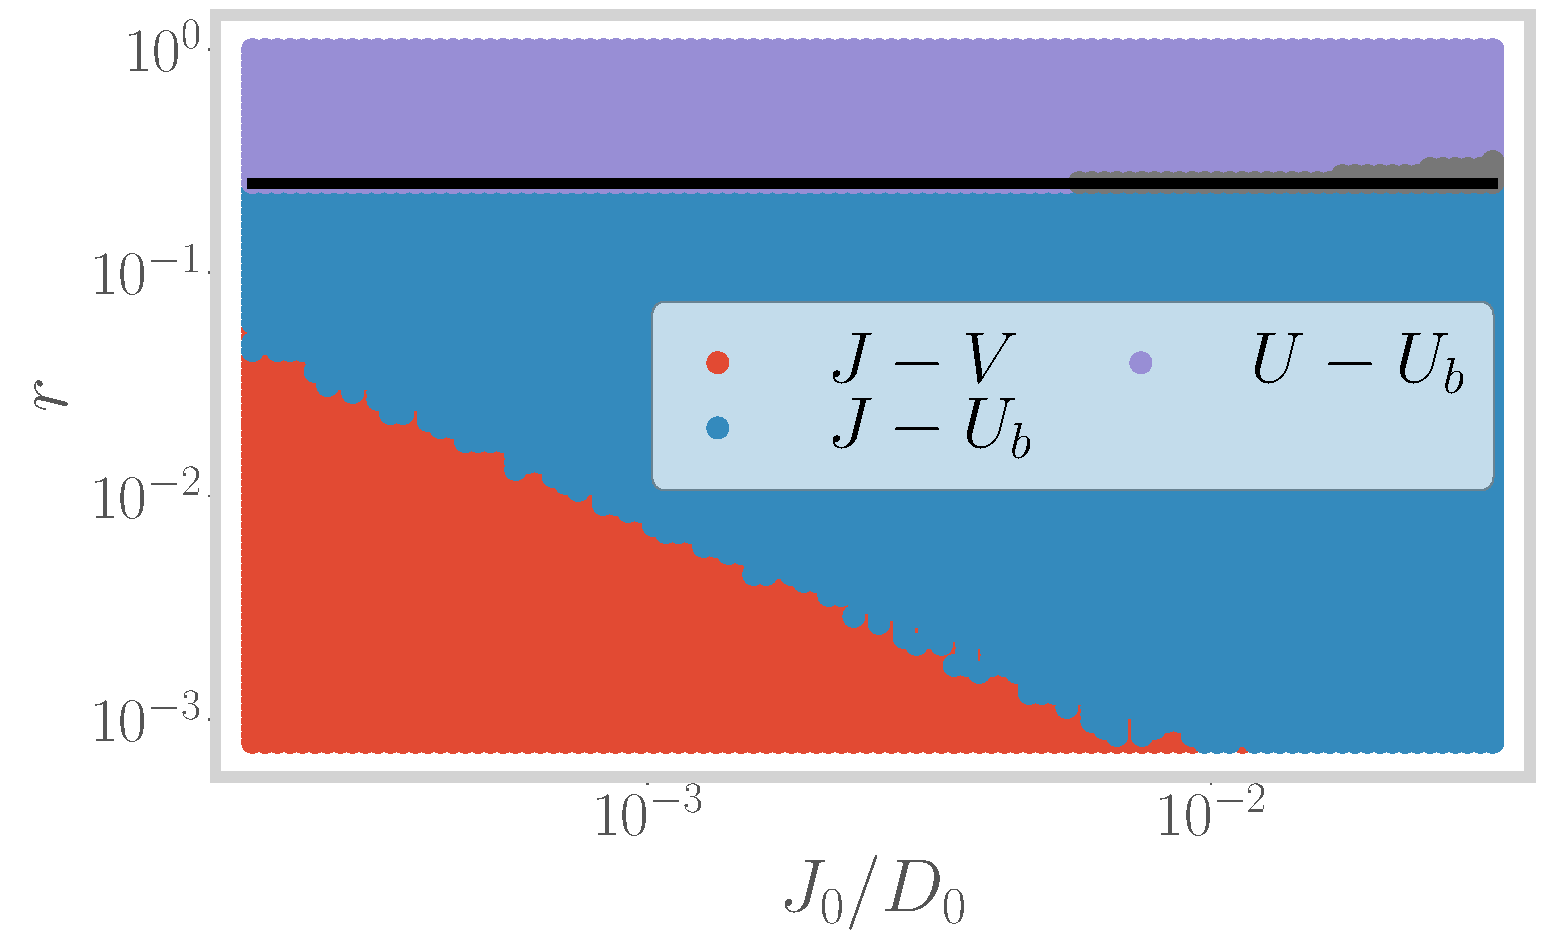
\includegraphics[width=0.48\textwidth]{phase-map-MIT.pdf}
	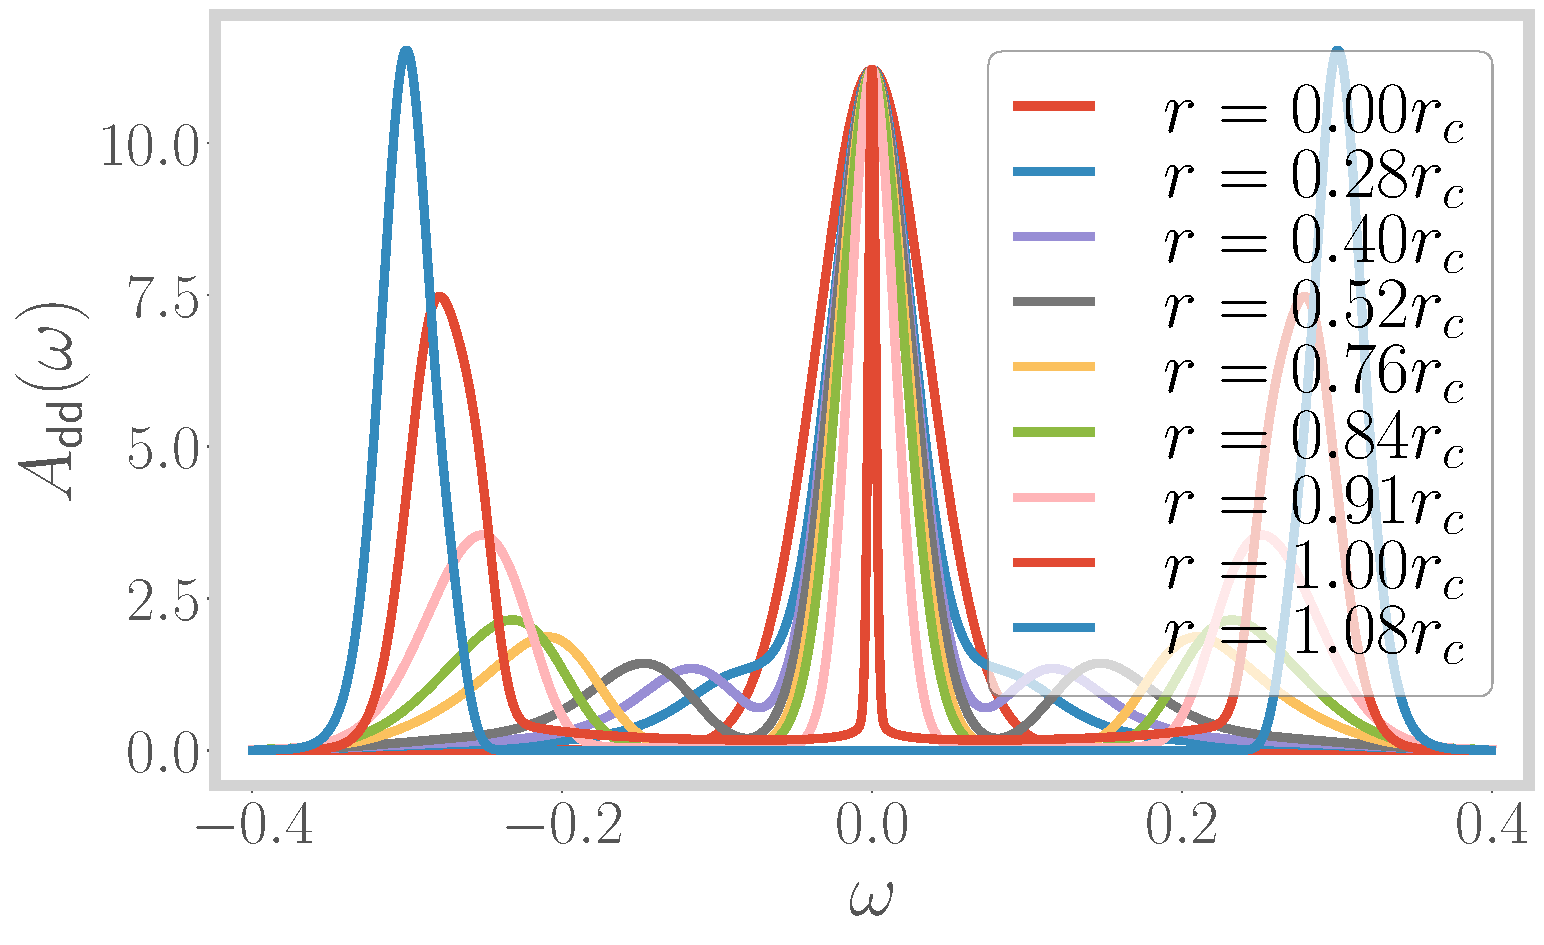
\includegraphics[width=0.48\textwidth]{spectral-function_dd.pdf}
	\caption{{\it Left:} Phase diagram of the extended SIAM auxiliary model. As the parameter \(r\) is tuned through 0.25, the metallic blue phase changes into the insulating violet phase. {\it Right:} Local spectral function of the auxiliary model. It shows a hard gap for \(r/r_c > 1\).}
	\label{spec_func_mit}
\end{figure}

The impurity local spectral function \(\mathcal{A}_{dd}(\omega)\) and the impurity-bath real space off-diagonal spectral function \(\mathcal{A}_{dz}(\omega)\) reveal a gap in the spectrum at low \(\omega\) for \(U_b > J/4\). We show the former in fig.~\ref{spec_func_mit}. The gap in the former shows the absence of any gapless excitations that can allow the impurity configuration to fluctuate, while the vanishing of the off-diagonal spectral function shows that this is because the entanglement between the impurity and the bath has been quenched. 

In Fig.~\ref{spin-charge-correlations}, we show the behaviour of the spin-flip and charge isospin-flip correlations between two neighbouring real space sites, as well as the mutual real space entanglement and mutual information. Both show a sharp fall on crossing the transition, demonstrating the destruction of the Kondo cloud and the stabilisation of the local moment on the impurity. Importantly, they charge correlations show a rise very close to the transition (can be seen as a single elevated blue point near \(r = 0.25\) in the left panel of Fig.~\ref{spin-charge-correlations}); this indicates that the transition is precipitated by the growth of pairing correlations.

\begin{figure}[!htb]
\centering
	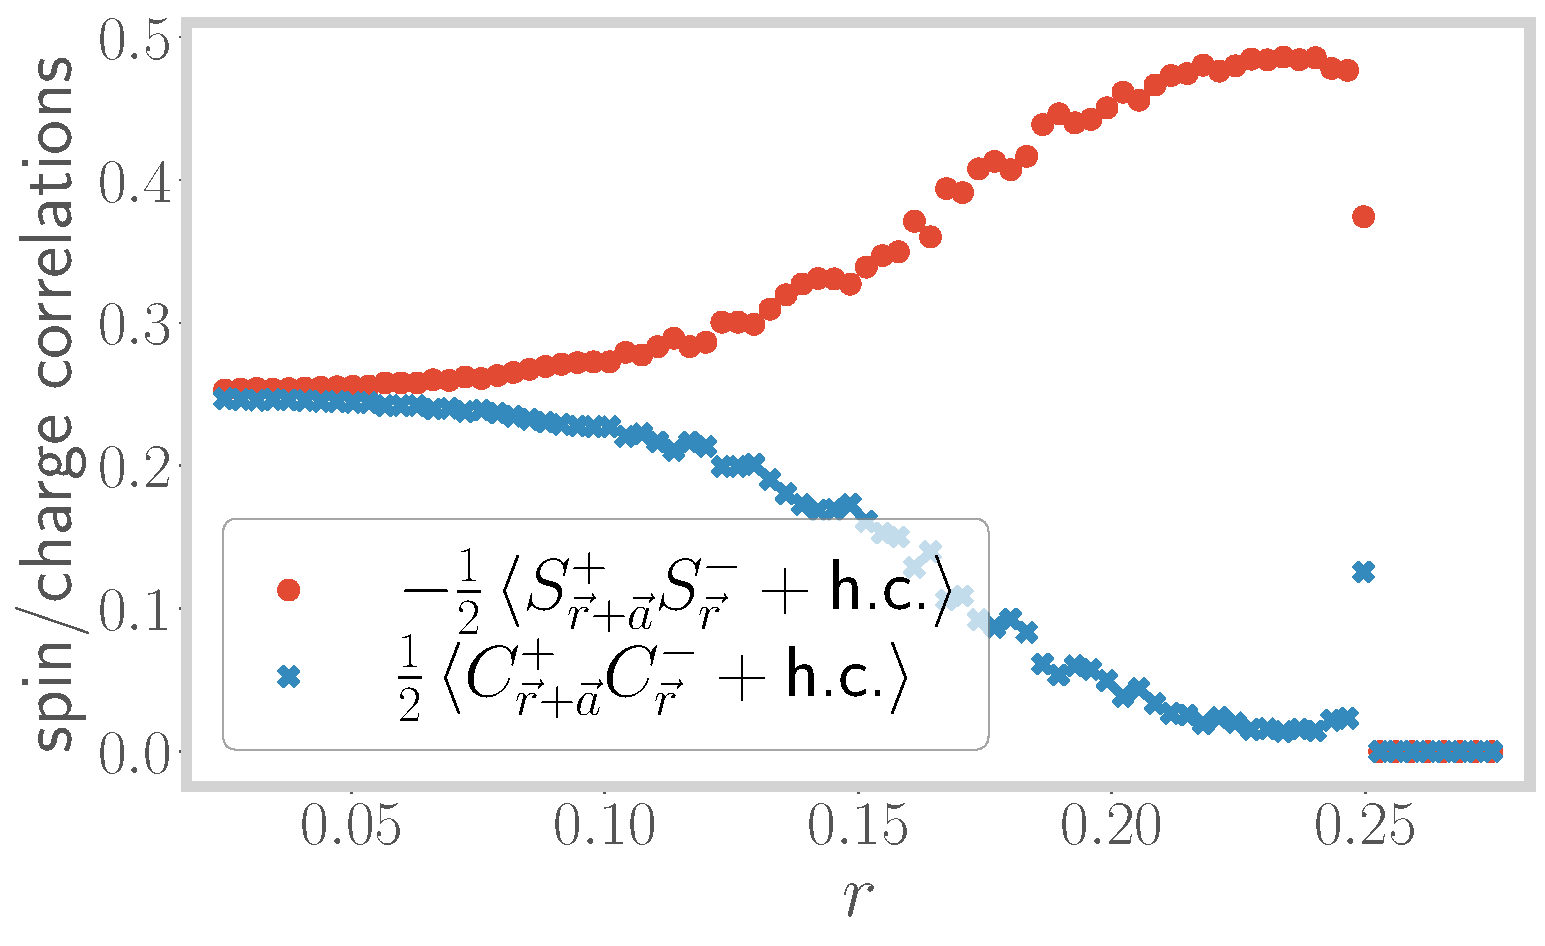
\includegraphics[width=0.48\textwidth]{spin-charge-corr-full.pdf}
	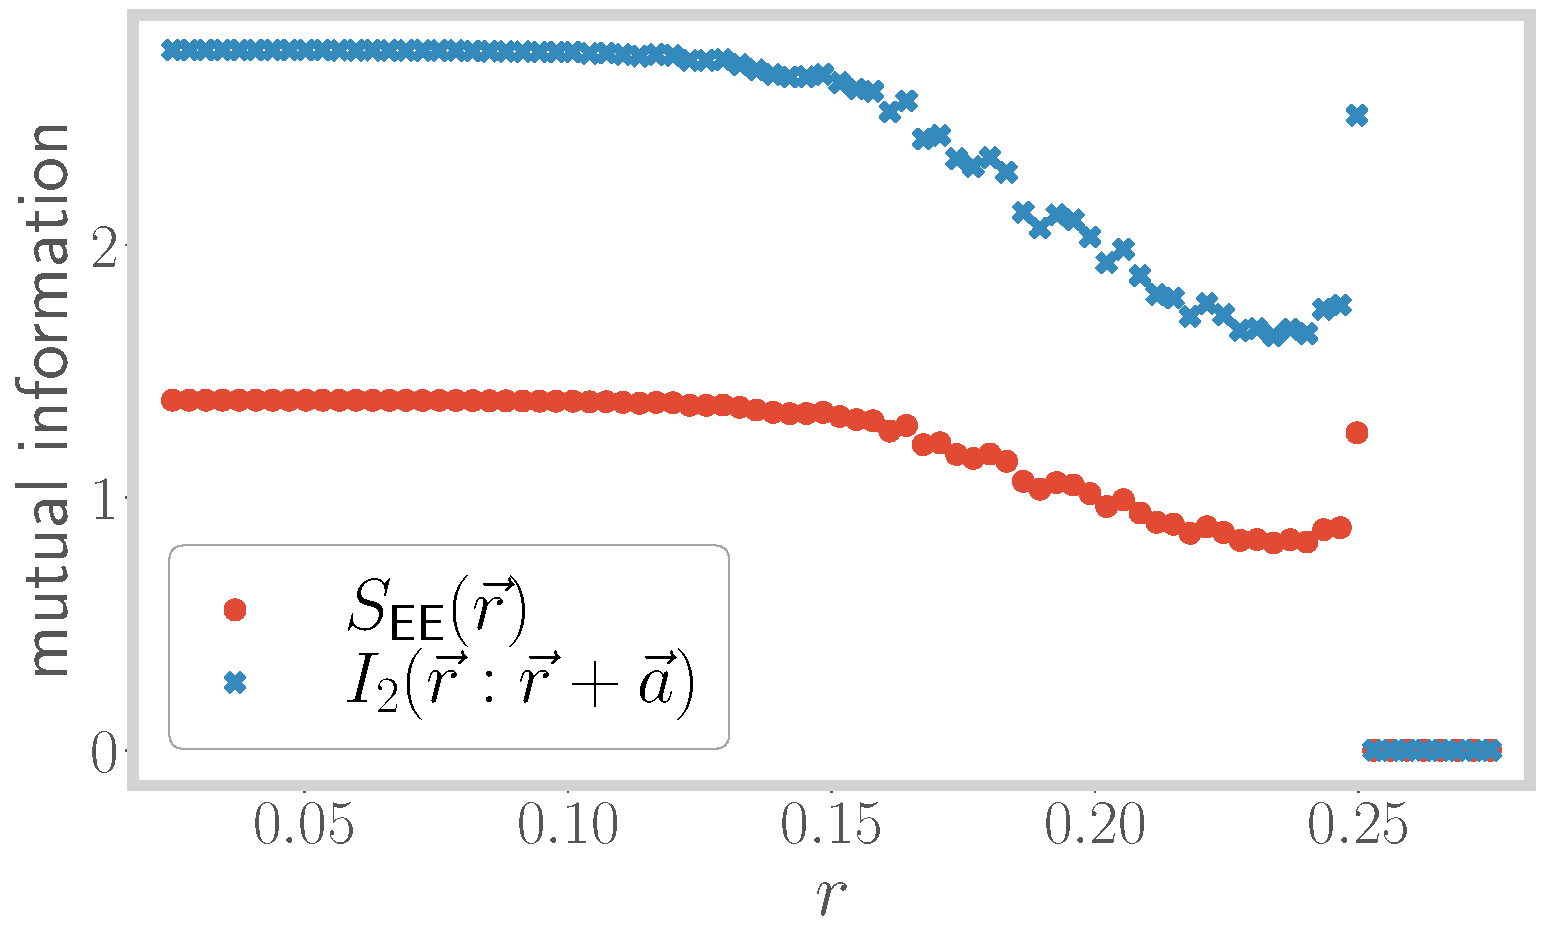
\includegraphics[width=0.48\textwidth]{impEE-mutinfo-d0.pdf}
	\caption{{\it Left}: Spin-flip correlations(red) and charge-flip correlations(blue) in real space. The former increases as the system moves into the Kondo regime, and then vanishes at the transition. The latter decreases as the charge content is removed from the ground state in the Kondo regime, but shows a sudden increase at the transition. {\it Right}: Real space Entanglement and mutual information. Both vanish in the local moment phase.}
	\label{spin-charge-correlations}
\end{figure}

\subsection{Value of the critical paramter for the bulk model}
Using the mappings between the auxiliary model parameters and the bulk parameters (eq.~\ref{map_aux_bulk}), one can define a critical value \(r^{*}\) of the ratio \(r = U_{H-H}/J_{H-H}\) at the critical points \(-U_b/J=1/4\) \textit{for a given and fixed value of \(U\)}. We will now argue that this critical point describes a metal-insulator transition. For \(r < r^{*}\), the well-defined low-\(\omega\) central peak in the impurity spectral function, as well as the large mutual and information correlations, in the ground state, among the members of the Kondo cloud or between the impurity and the zeroth site show that the impurity and the bath are very strongly entangled. This means that both the local and the nearest-neighbour Greens functions have poles at low\(-\omega\) and support the propagation of electrons through gapless excitations. Since the spectral function is also very simply related to that of the auxiliary model, the former also shows the same zero-energy resonance. 

On the other side \(r > r^{*}\) of the critical point, we know that the impurity gets decoupled from the bath, leading to the transformation of poles into zeros in the Greens functions. This is demonstrated through the gapping of the impurity spectral function in fig.~\ref{spec_func_mit}, and it describes an insulating phase where the electrons get "jammed" in the local states. By the same argument as above, the bulk spectral function also sees a gap in this phase when the impurity spectral function is gapped.

Finally, using relations \eqref{map_aux_bulk} between the auxiliary model couplings and the bulk parameters, we can offer a functional form for the critical value of the parameter $r^{*} = U_{H-H}^{*}/J_{H-H}^{*}$. Using \(U_{H-H}^{*} = U^* + U_b\) and \(J_{H-H}^{*} = 2J^*\) (following \eqref{map_aux_bulk}), we get
\begin{equation}\begin{aligned}
	r^{*} &=& \frac{1}{2}\left(\frac{U^{*}}{J^{*}} + \frac{U_b}{J^*}\right)
\end{aligned}\end{equation}
where $U^{*}$ and $J^{*}$ are the values of the on-site and Kondo couplings of the auxiliary model at the auxiliary model (i.e., the extended SIAM with a correlated bath) at the transition between the Kondo screened and the local moment phases. By using the auxiliary model criticality condition \(-4U_b = J^*\), the bulk criticality parameter \(r^*\) takes the form
\begin{equation}\begin{aligned}
	r^{*} &=& \frac{1}{2}\left(\frac{U^{*}}{J^{*}} - \frac{1}{4}\right)
\end{aligned}\end{equation}
Parametrising the bath correlation coupling as $U_{b}=-\frac{U}{10}$, we obtain $U^{*}/J^{*}=5/2$, and $r^{*} = 9/8$ for the 2D square lattice Hubbard-Heisenberg model. The reduction in the value of \(r\) from \(2.5\) in the auxiliary model to \(~1.1\) in the bulk model can be attributed to (i) the reduction in the effective bulk repulsion \(U\) due to the competition coming from the attractive \(U_b\), and (ii) increased hybdridisation through \(J\) due to the presence of multiple auxiliary models that connect two lattice sites.

\section{Momentum-space picture of the MIT}
In order to understand the nature of the transition in momentum space, we employ the expression obtained in the previous sections and compute the spectral function, self-energy and correlation functions in the top right quadrant of the first Brillouin zone. We first show the \(k-\)space spectral functions near zero frequency, in Fig.~\ref{kspace_specfunc}.

\begin{figure}[!htb]
\centering
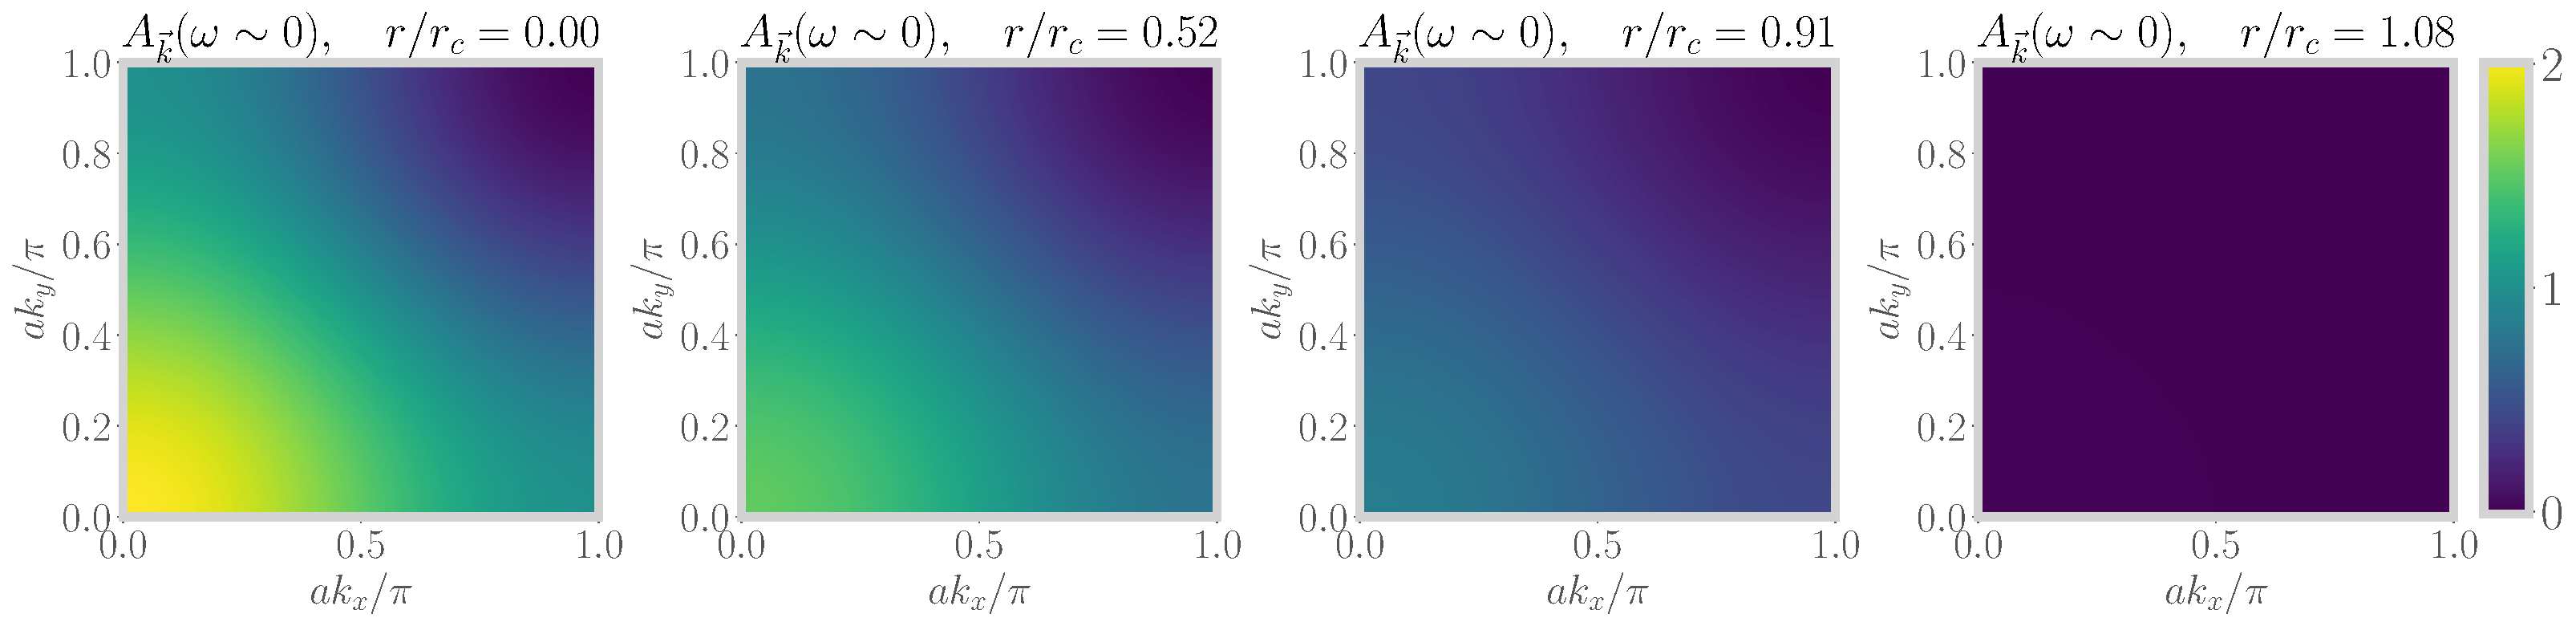
\includegraphics[width=\textwidth]{kspace-spectral-function-all.pdf}\hspace{\fill}
\caption{\(k-\)space dependence of single-particle spectral function, \(A_{\vec k}(\omega \sim 0)\), at four values of the tuning parameter \(r\). The \(\vec k\) values are taken from the top right quadrant of the first Brillouin zone. In the metallic phase (\(r < r_c\)), the spectral function shows a \(k-\)dependence, indicating the presence of gapless excitations. Close to the transition (and beyond it), the momentum dependence gets removed and there is no spectral weight left in the infrared regime.}
\label{kspace_specfunc}
\end{figure}

In Fig.~\ref{kspace_selfenergy}, we plot the momentum dependence of the single-particle self-energy, similar to the spectral function. The self-energy is flat in \(k-\)space away from the transition, consistent with the fact that the correlations are small in that regime. Close to the transition, the correlations pick up, and lead to a momentum-dependence of the self-energy, renormalising the Fermi liquid in the process and ultimately destroying it.
\begin{figure}[!htb]
\centering
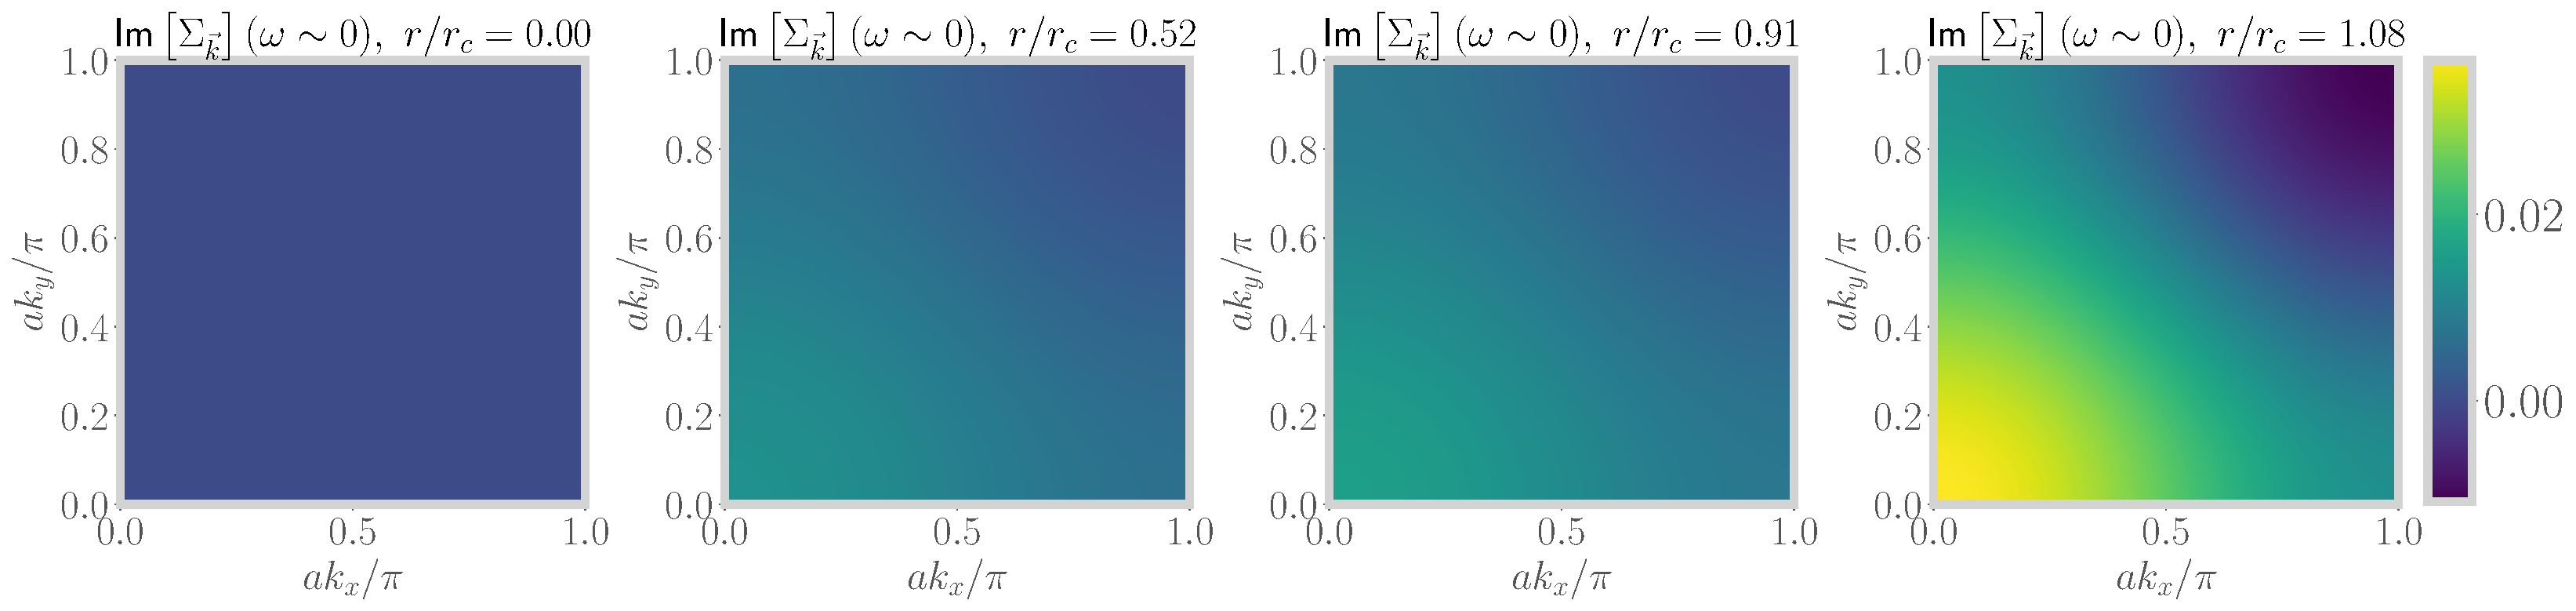
\includegraphics[width=\textwidth]{kspace-imagsigma-all.pdf}\hspace{\fill}
\caption{\(k-\)space dependence of imaginary part of the self-energy, \(\Sigma_{\vec k}(\omega \sim 0)\), at four values of the tuning parameter \(r\). In the metallic phase (\(r \ll r_c\)), the self-energy is quite small, indicating that the phase consists of an uncorrelated Fermi liquid. It increases close to the transition (and beyond it).}
\label{kspace_selfenergy}
\end{figure}

In Figs.~\ref{spin_kspace},\ref{charge_kspace} and \ref{pair_kspace}, we show the momentum dependence of two-particle correlation functions. In every figure, each panel shows the variation along a specific horizontal cut \(k_y=\text{constant}\), as a function of \(r\). Moving from the left panel to the right is equivalent to moving upwards in the top right quadrant of the first Brillouin zone. In each panel, moving upwards amounts to tuning the system towards the transition. The spin-spin correlations (in Fig.~\ref{spin_kspace}) are large near the \(\vec k = \left( 0,0 \right) \) point, presumably because of the dominance of the Kondo cloud at long wavelengths. They vanish in the local moment phase (flat blue region near the top). The charge and pairing correlations (Figs.~\ref{charge_kspace} and \ref{pair_kspace}) disappear as the system moves into the Kondo regime, but reappear exactly at the transition. This is tied to the non-Fermi liquid theory at the QCP, as seen in the auxiliary model.
\begin{figure}[!htb]
\centering
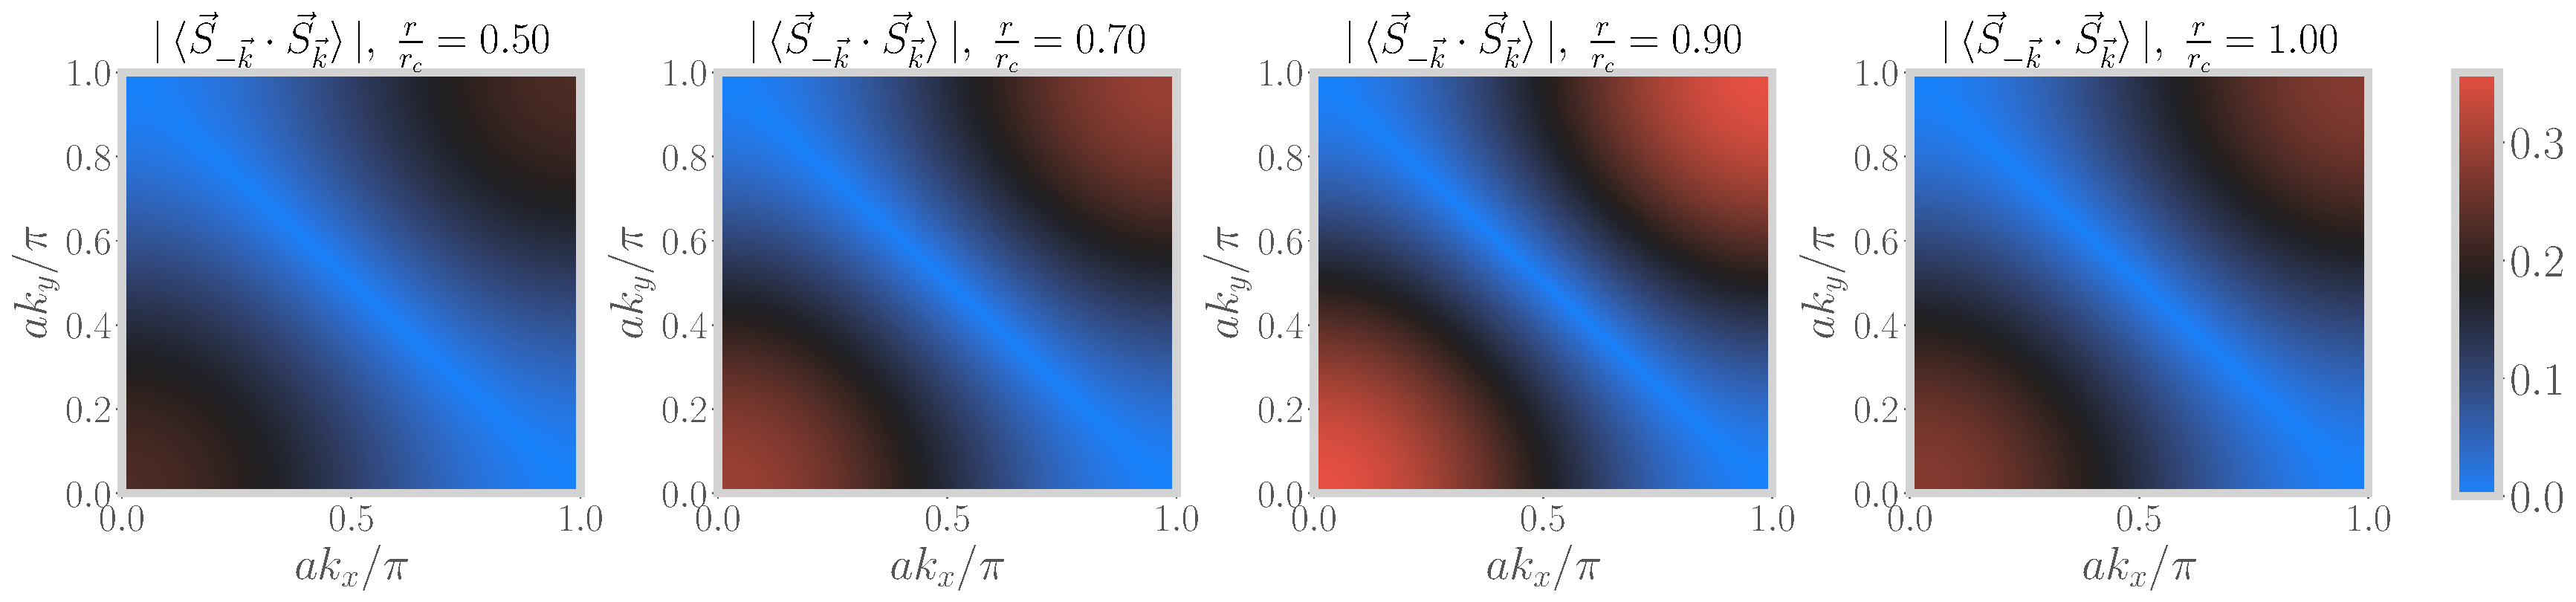
\includegraphics[width=\textwidth]{spin_rspace_all.pdf}
\caption{Momentum dependence of spin-spin correlation \(\left<\vec{S}_{-\vec k}\cdot\vec{S}_{\vec k} \right>\). Each frame shows the variation along a specific horizontal cut \(k_y=\text{constant}\), as a function of \(r\). Moving from the left figure to the right figure is equivalent to moving upwards in the top right quadrant of the first Brillouin zone. In each figure, moving upwards amounts to tuning the system towards the transition. The flat blue region at the top is the local moment phase, void of any non-local correlations.}
\label{spin_kspace}
\end{figure}

\begin{figure}[!htb]
\centering
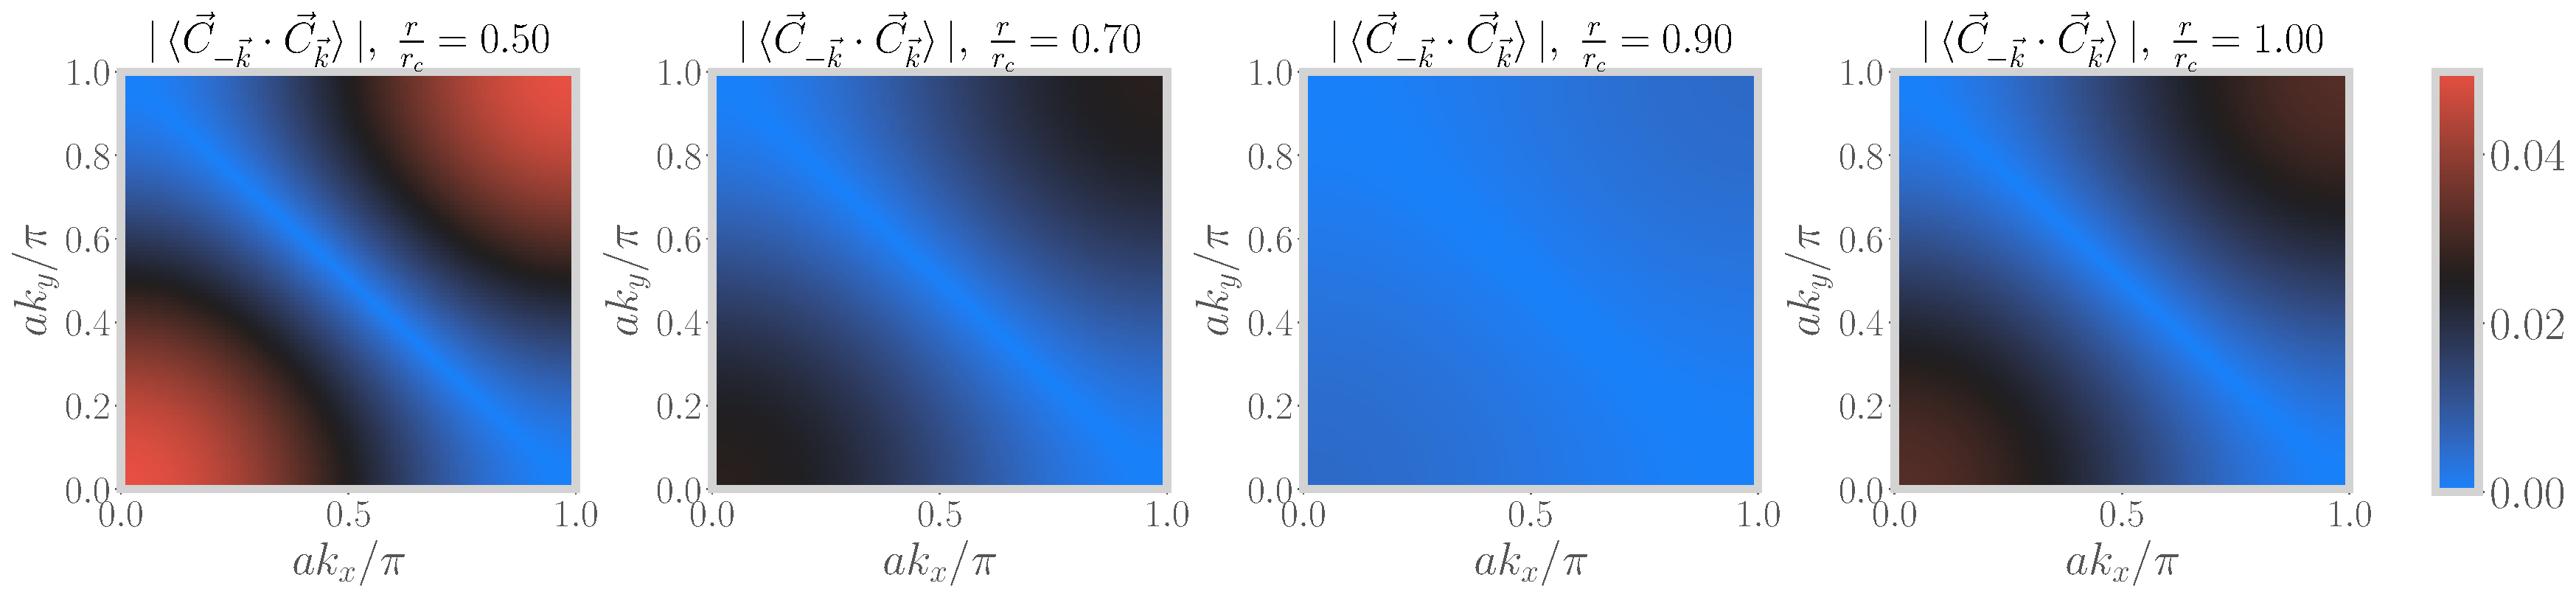
\includegraphics[width=\textwidth]{charge_rspace_all.pdf}
\caption{Momentum dependence of charge-charge correlation \(\left<\vec{C}_{-\vec k}\cdot\vec{C}_{\vec k} \right>\), where \(\vec C\) is the charge isospin associated with the doublet formed by the doublon and holon states. Each frame shows the variation along a specific horizontal cut \(k_y=\text{constant}\), as a function of \(r\). Moving from the left figure to the right figure is equivalent to moving upwards in the top right quadrant of the first Brillouin zone. In each figure, moving upwards amounts to tuning the system towards the transition. The flat blue region at the top is the local moment phase, void of any non-local correlations.}
\label{charge_kspace}
\end{figure}

\begin{figure}[!htb]
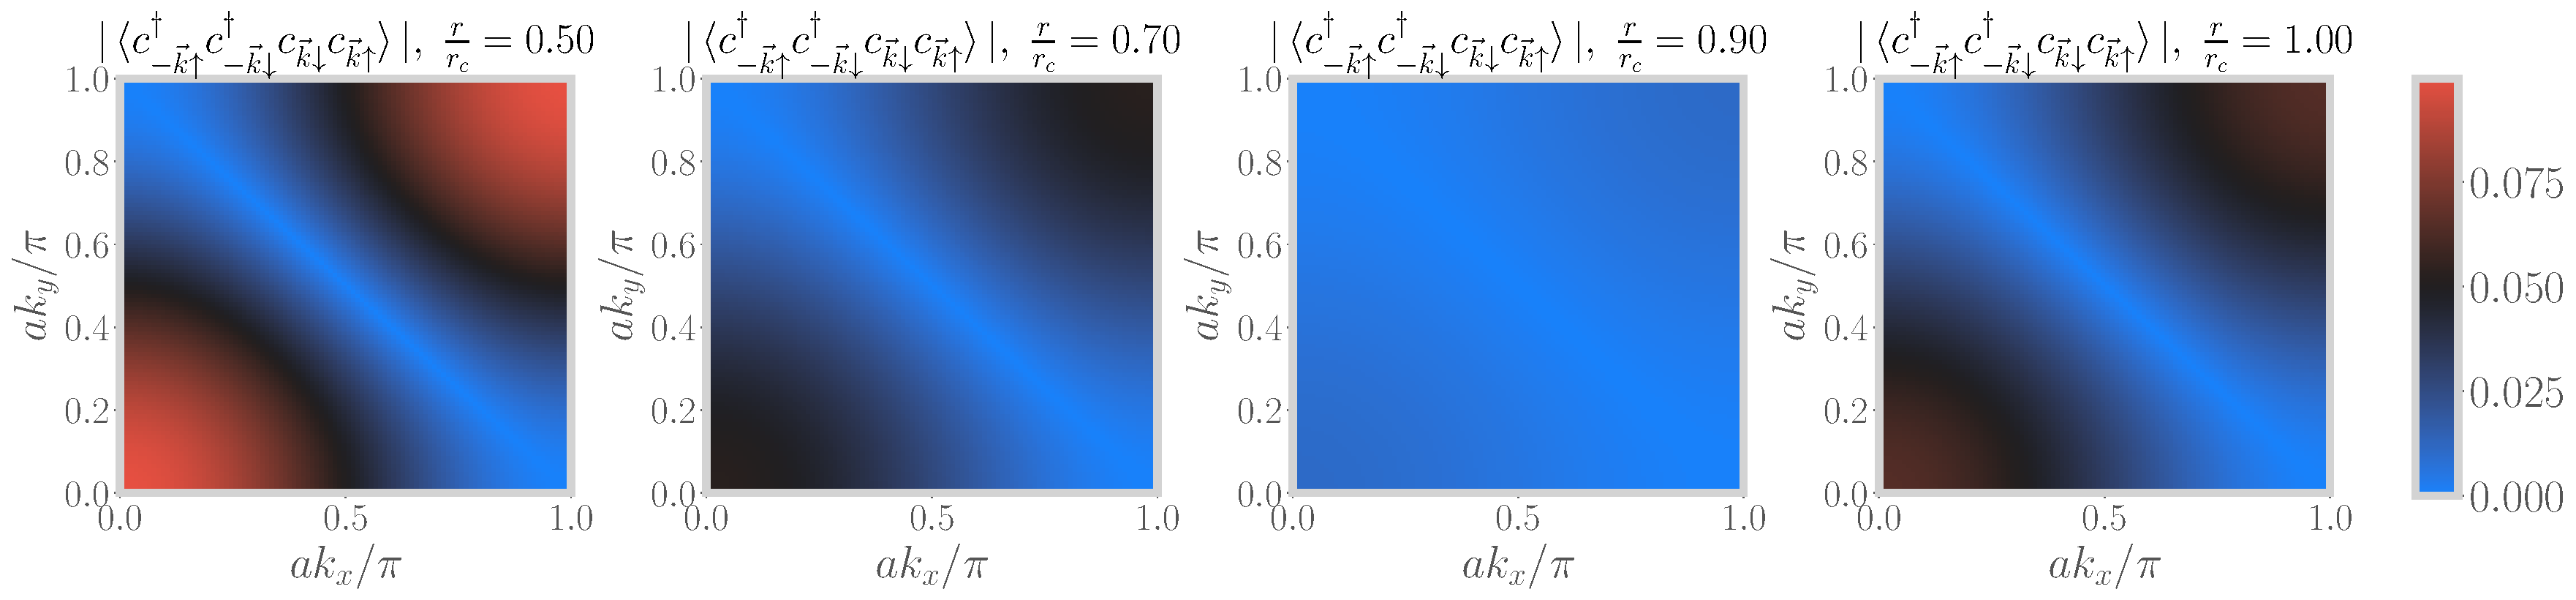
\includegraphics[width=\textwidth]{pair_rspace_all.pdf}
\caption{Momentum dependence of pairing correlation \(\left<c^\dagger_{-k\uparrow}c^\dagger_{-k\downarrow}c_{k\downarrow}c_{k\uparrow}\right>\). Each frame shows the variation along a specific horizontal cut \(k_y=\text{constant}\), as a function of \(r\). Moving from the left figure to the right figure is equivalent to moving upwards in the top right quadrant of the first Brillouin zone. In each figure, moving upwards amounts to tuning the system towards the transition. The flat blue region at the top is the local moment phase, void of any non-local correlations.}
\label{pair_kspace}
\end{figure}

\begin{figure}[!htb]
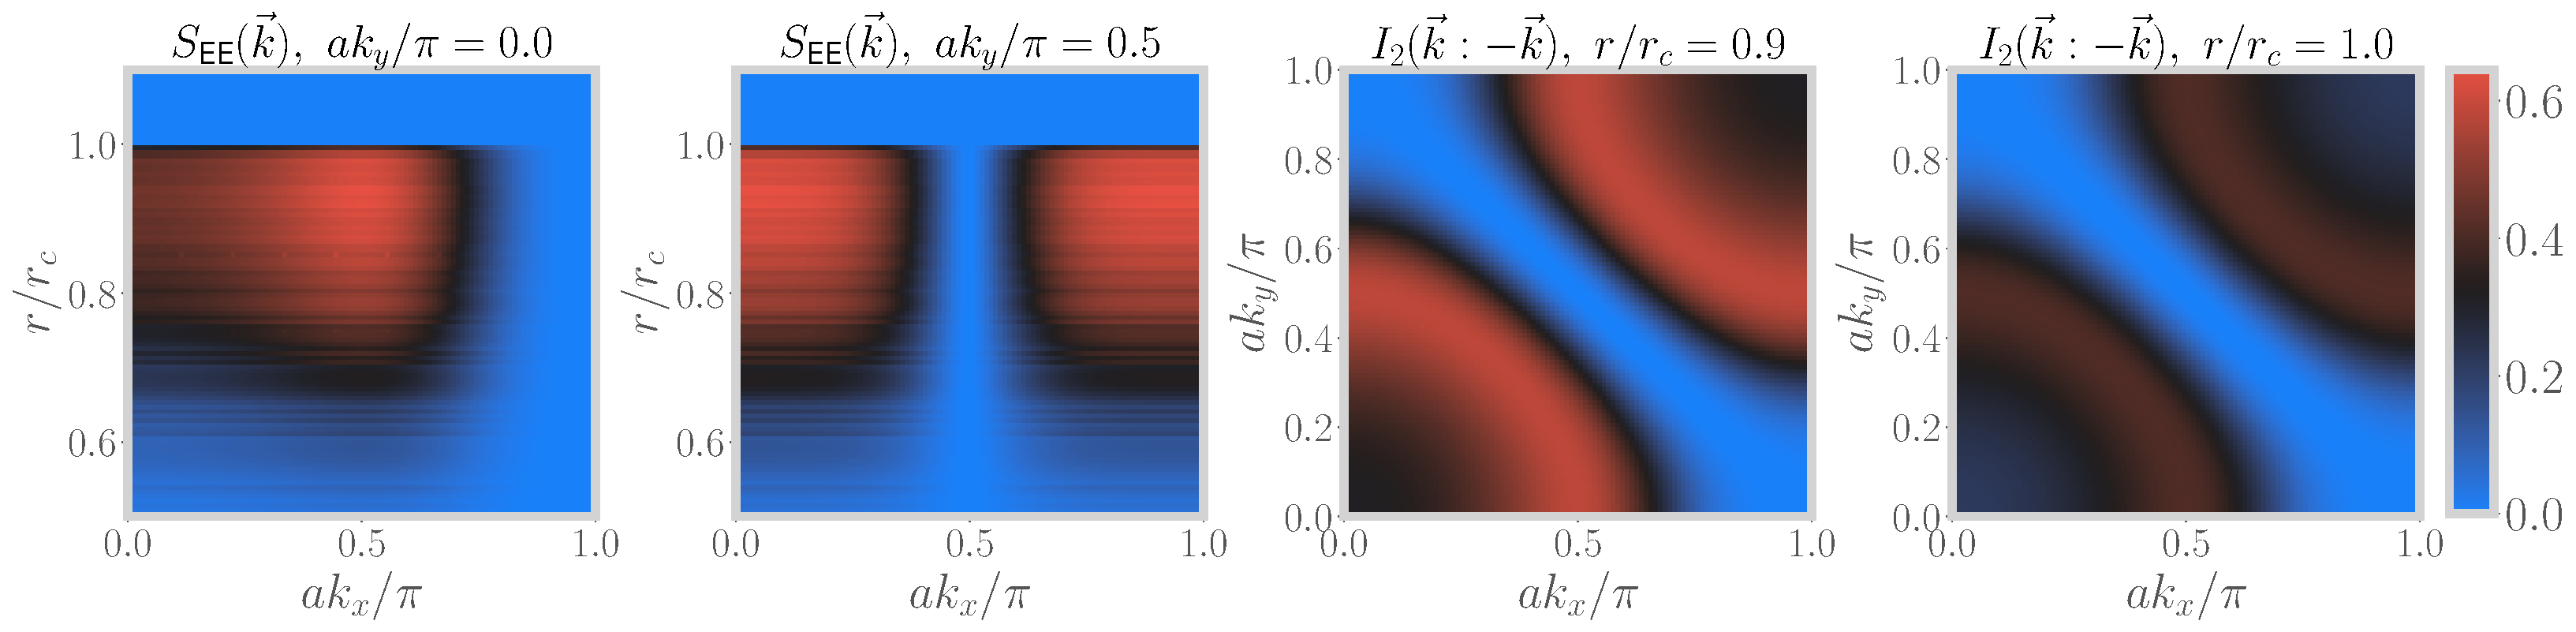
\includegraphics[width=\textwidth]{vne_kspace_all.pdf}
\caption{Momentum dependence of \(k-\)space von Neumann entanglement entropy \(S_\text{EE}(\vec k)\) and \(k-\)space mutual information \(I_2(\vec k:-\vec k)\). The first two frames (from the left) show the variation in entanglement of a \(k-\)space in the \(k_x\) direction as the transition parameter \(r\) is tuned through the metal-insulator transition, for two values of \(k_y\). The last two frames show the distribution of mutual information between two states \(\vec k\) and \(-\vec k\), in the \(k_x-k_y\) plane, for two values of \(r\). \(r/r_c=0.9\) represents a highly correlated metal, while \(r/r_c=1\) represents the non-Fermi liquid metal formed at the transition.}
\label{entanglement_kspace}
\end{figure}

{\color{blue} In order to provide a second way of visualising these correlations, we have provided some videos that show their variation in the \(k_x-k_y\) plane as a function of \(r/r_c\). The videos for the spin-spin correlation and the pairing correlations are named ``ss\_rspace.gif" and ``pairing\_rspace.gif", respectively. Each frame of the video shows a colourmap of the correlation in the top right quadrant of the first Brillouin zone, at a {\it specific value of \(r\)}. The movie then shows the {\it evolution of this \(k-\)space colourmap} as \(r\) is tuned towards and into the transition.}

\section{Emergence of effectively pseudogapped Anderson model at the MIT}
%\begin{itemize}
%\item 
We begin by recalling that the RG equation (in the weak coupling limit) of the \(J-U_b\) model that emerges in the Kondo limit of the eSIAM is similar to that of the pseudogapped Anderson model~\cite{fritzvojta2004} that has a bath density of states of the form \(\rho\sim |\omega|^\alpha\). If we define the dimensionless Kondo coupling \(g = \rho J\) and the dimensionless bath coupling \(u = \rho U_b\), the RG equation for \(g\),
\begin{equation}\begin{aligned}
	\Delta g \simeq g^2 + 4gu~,
\end{aligned}\end{equation}
can be mapped to the corresponding RG equation for the pseudogapped Kondo model,
\begin{equation}\begin{aligned}
	\Delta g = g^2 - \alpha g~,
\end{aligned}\end{equation}
with the identification \(\alpha = -4u = -4\rho U_b\). Specifically, this corresponds to a Kondo model that is coupled to a conduction bath with a single-particle density of states that is vanishing (pseudogapped): $\rho\sim |\omega|^{\alpha}$~.
\par
Now, following the work by Si and Kotliar~\cite{kotliarsi_1993}, the impurity self-energy of the \(J-U_b\) model takes the form
	\begin{equation}\begin{aligned}
		\Sigma_{dd} \sim |\omega|^{\gamma_{dd}}~,
	\end{aligned}\end{equation}
	where the exponent \(\gamma_{dd}\) can be written in terms of the phase shifts (at the RG fixed point) \(\delta^*_\text{sp}\) and \(\delta^*_\text{ch}\) suffered by the conduction electrons due to the potentials \(J\) and \(U_b\) respectively in the Hamiltonian:
	\begin{equation}\begin{aligned}
		\gamma_{dd} = \frac{5}{4} - \left[ \frac{1}{\pi}\left( \delta^*_\text{sp} + \delta^*_\text{ch} \right) - \frac{1}{2}  \right]^2 - \left( \frac{\delta^*_\text{ch}}{\pi} \right)^2~.
	\end{aligned}\end{equation}
	The phase shifts are given by \(\delta^*_\text{sp}=\arctan\left( \pi g/2 \right) \) and \(\delta^*_\text{ch}=\arctan\left( \pi u/2 \right) \). In the small coupling limit, these can be approximated as \(\delta^*_\text{sp}=\pi g/2\) and \(\delta^*_\text{ch}=\pi u/2\).
\par 
We now focus on the quantum critical point \(g = -4u\) of our model. At this point, the phase shifts get related to each other: \(\delta^*_\text{sp} = -4\delta^*_\text{ch}\), so that the exponent of the self-energy takes the form
	\begin{equation}\begin{aligned}
		\gamma_{dd} \simeq 1 - \frac{3}{\pi}\delta^*_\text{ch} = 1 + \frac{3}{8}\alpha
	\end{aligned}\end{equation}
	where we have used the fact that for our model, the effective pseudogap parameter \(\alpha\) is set to \(-4u\). The local self-energy then vanishes as
	\begin{equation}\begin{aligned}
		\Sigma_{dd} \sim |\omega|^{\gamma_{dd}} = |\omega|^{1 + \frac{3}{8}\alpha}
	\end{aligned}\end{equation}
The power-law exponent $\gamma_{dd}=1 + \frac{3}{8}\alpha$ lies in the following range: $1\leq \gamma_{dd} \leq 2$. This can be compared with the expression \(\sim|\omega|^{2-3\alpha}\) of the impurity self-energy obtained in ref.~\cite{fritzvojta2004} where the power law exponent ranges between $1/2$ and $2$. In a similar manner, the self-energy \(\Sigma_{dz}\) for scattering processes that connect the impurity site and the bath zeroth site can also be obtained. The exponent \(\gamma_{dz}\) for this self-energy is given by \(\gamma_{dz} = 2 - 2\gamma_{dd}\), so that this non-local self-energy diverges as
\begin{equation}\begin{aligned}
	\Sigma_{dz} \sim |\omega|^{- \frac{3}{4}\alpha}~.
\end{aligned}\end{equation}
The divergence of the non-local self-energy \(\Sigma_{dz}\) leads to the vanishing of the nearest-neighbour Greens function \(\mathcal{G}_{dz}\) as \(\omega \to 0\): 
\begin{equation}\begin{aligned}
	\mathcal{G}_{dz}(\omega)  \sim 1/(\mathcal{G}_{dz}^{-1} - \Sigma_{dz}(\omega)) \sim \omega^{3\alpha/4}.
\end{aligned}\end{equation}

By using our tiling approach (eq.~\ref{k_Gf_siam}), the \(k-\)space Greens function of the lattice problem, at the critical point, can be shown to become independent of the momentum, through the vanishing of the momentum dependent contribution coming from \(\mathcal{G}_{dz}\):
\begin{equation}\begin{aligned}
	G_\text{H-H}(\vec k,\omega) = G_\text{loc}(\omega) + \frac{\xi_{\vec k}}{\lambda_{\vec k_0}^2\mathcal{W}}\mathcal{G}_{dz}(\omega) = G_\text{loc}(\omega)
\end{aligned}\end{equation}
This leads to the spectral function \(A(\omega,\vec k)\) losing all momentum dependence for the gapless excitations. Moreover, the self-energies vanish .

It is clear that the divergent $\Sigma_{dz}$ does not affect the single-particle self-energy $\Sigma(\vec k,\omega)$ precisely at the Fermi surface, i.e., for $\xi_{\vec{k}}= 0$; $\Sigma(\vec k,\omega)$ diverges everywhere else in the Brillouin zone. This corresponds to a gapless non-Fermi liquid metal present at the QCP, corresponding to a system with Landau quasiparticle poles precisely on the Fermi surface but which are destroyed everywhere else. Now, following the arguments laid out in Ref.\cite{sujan2023}, the single-particle spectral function $A(\omega,\vec{k})$ will vanish (i.e., be pseudogapped) for excitations away from the Fermi surface
\begin{equation}
A(\omega,\vec{k}) \sim \frac{1}{\mathcal{W}}\xi_{\vec k}|\omega|^{\frac{3}{4}\alpha}~.
\end{equation}	
This clearly corresponds to the vanishing of the residue of the Landau quasiparticle precisely at the metal-insulator transition, and the emergence of a gapless non-Fermi liquid ``local quantum critical" metal~\cite{Si2001}. Further, the fact that the single-particle self-energy $\Sigma$ vanishes precisely at the Fermi surface signals the fact that the Luttinger's count for states on the Fermi surface is preserved and identical to that in the Fermi liquid phase. 


\section{Topological nature of the transition}
Since the impurity charge hybridising with the bath contributes to the total Luttinger volume of the system~\cite{martin1982fermi}, decoupling of the impurity from the conduction bath leads to a difference in the value of the Luttinger volume between the local moment (LM) and the strong-coupling (SC) fixed points. If we define \(\mathcal{N}_L\) as the Luttinger volume with the spin-degeneracy accounted for, we can write
\begin{equation}\begin{aligned}
	\label{lutt_change}
	\mathcal{N}_L^\text{lm} - \mathcal{N}_L^\text{sc} = 1
\end{aligned}\end{equation}
where \(\mathcal{N}_L^\text{lm},\mathcal{N}_L^\text{sc}\) are the Luttinger volumes at the local moment and strong-coupling fixed points respectively. This equation expresses the fact that the Luttinger volume of the bath increases by \(1\) when the system is tuned from LM to SC, and this happens because the single-particle impurity excitation in the lower-Hubbard at the atomic limit gets transferred to the bath Greens function in the process. The quantity which tracks this transfer is therefore \(\mathcal{N}_\text{imp}\), the number of poles minus the number of zeros in the impurity Greens function at and below the Fermi surface:
\begin{equation}\begin{aligned}
	\label{imp_count_def}
	\mathcal{N}_\text{imp} = \begin{cases}
		1 & \text{ at LM}\\
		0 & \text{ at SC}
	\end{cases}\implies \Delta \mathcal{N}_\text{imp} = 1
\end{aligned}\end{equation}
The Luttinger volume \(\mathcal{N}_L\) is related to this impurity count by the equation
\begin{equation}\begin{aligned}
	\mathcal{N}_L = \mathcal{N} - \mathcal{N}_\text{imp}
\end{aligned}\end{equation}
where \(\mathcal{N}\) is the total number of electrons in the system, accounting for the spin degeneracy. If we keep this total number fixed (isolated system), the changes in the impurity count and Luttinger volume become constrained: 
\begin{equation}\begin{aligned}
	\Delta \mathcal{N}_L = - \Delta \mathcal{N}_\text{imp}~.
\end{aligned}\end{equation}
Eq.~\ref{imp_count_def} then readily implies eq.~\ref{lutt_change}.

In order to connect this impurity topological change with the bulk model, we write the total number of particles in the bulk system in the following manner:
\begin{equation}\begin{aligned}
	\mathcal{N} = \mathcal{N}_\text{loc} + \mathcal{N}_\text{deloc}
\end{aligned}\end{equation}
\(\mathcal{N}_\text{loc}\) is the number of real poles minus the number of zeros of the local Greens function. \(\mathcal{N}_\text{deloc}\) is the number of real poles minus the number of zeros of the \(k-\)space Greens functions. The former (latter) contributes only in the insulating (metallic) phase, because in the metallic (insulating) phase, the local (\(k-\)space) Greens function develop imaginary self-energy and the real poles in these Greens functions get replaced by imaginary poles. Together, these two terms accurately count the total number of particles in both these phases. These two terms are defined as
\begin{equation}\begin{aligned}
	\mathcal{N}_\text{loc} = \sum_i \mathcal{N}_i = \oint \frac{dz}{2\pi i}n_F(z) \text{Tr}\left[G_i(z)\right], ~ ~ ~\mathcal{N}_\text{deloc} = \sum_k \mathcal{N}_k = \oint \frac{dz}{2\pi i}n_F(z) \text{Tr}\left[G_k(z)\right] = \mathcal{N}_L
\end{aligned}\end{equation}
\(G_i(z)\) is the local Greens function at site \(i\) of the bulk model, and \(G_k(z)\) is the \(k-\)space Greens function in the bulk model. \(N_\text{deloc}\) is just the Luttinger volume \(\mathcal{N}_L\) of the bulk system. With this, the total number of particles in the bulk can be expressed as
\begin{equation}\begin{aligned}
	\label{bulk_total}
	\mathcal{N} = \sum_i \mathcal{N}_i + \mathcal{N}_\text{L}
\end{aligned}\end{equation}
From eq.~\ref{greens_func_relation}, we know that the bulk local Greens function is proportional to that of the auxiliary model, and that gives \(\sum_i \mathcal{N}_i = \mathcal{N}_\text{imp}\sum_i = \mathcal{N} \mathcal{N}_\text{imp}\). There we used the fact that for a half-filled system, the total number of sites is equal to the total number of particles in the system. Substituting this into eq.~\ref{bulk_total} and again using \(\Delta \mathcal{N} = 0\) gives
\begin{equation}\begin{aligned}
	\mathcal{N} = \mathcal{N} \mathcal{N}_\text{imp} + \mathcal{N}_\text{L} \implies \Delta \mathcal{N}_\text{L} = - \mathcal{N} \Delta \mathcal{N}_\text{imp}
\end{aligned}\end{equation}
We already know that \(\Delta \mathcal{N}_\text{imp}=1\) across the transition, so we get
\begin{equation}\begin{aligned}
	\mathcal{N}_L^\text{metal} - \mathcal{N}_L^\text{insulator} = \mathcal{N}\left(\mathcal{N}_\text{imp}^\text{sc} - \mathcal{N}_\text{imp}^\text{lm}\right) = \mathcal{N}
\end{aligned}\end{equation}
The metal-insulator transition is therefore characterised by a change in the topological quantity \(\mathcal{N}_L\). The topological nature arises from the fact that it can be expressed in terms of winding numbers related to the corresponding Greens functions. \(\mathcal{N}_\text{imp}\), which derives from the impurity Greens function \(G_d\), is related to the winding numbers of the curves \(\text{Det}[G_d^{-1}(\Gamma^<)]\) and \(\text{Det}[G_d^{-1}(\Gamma^0)]\). The winding number is simply the number of times this function encircles the origin when traced on the curves \(\Gamma^<\) and \(\Gamma^0\) that enclose all poles inside and on the Fermi surface respectively. An example of such a winding number is shown in fig.~\ref{imp_winding}.
\begin{figure}[!htb]
	\centering
	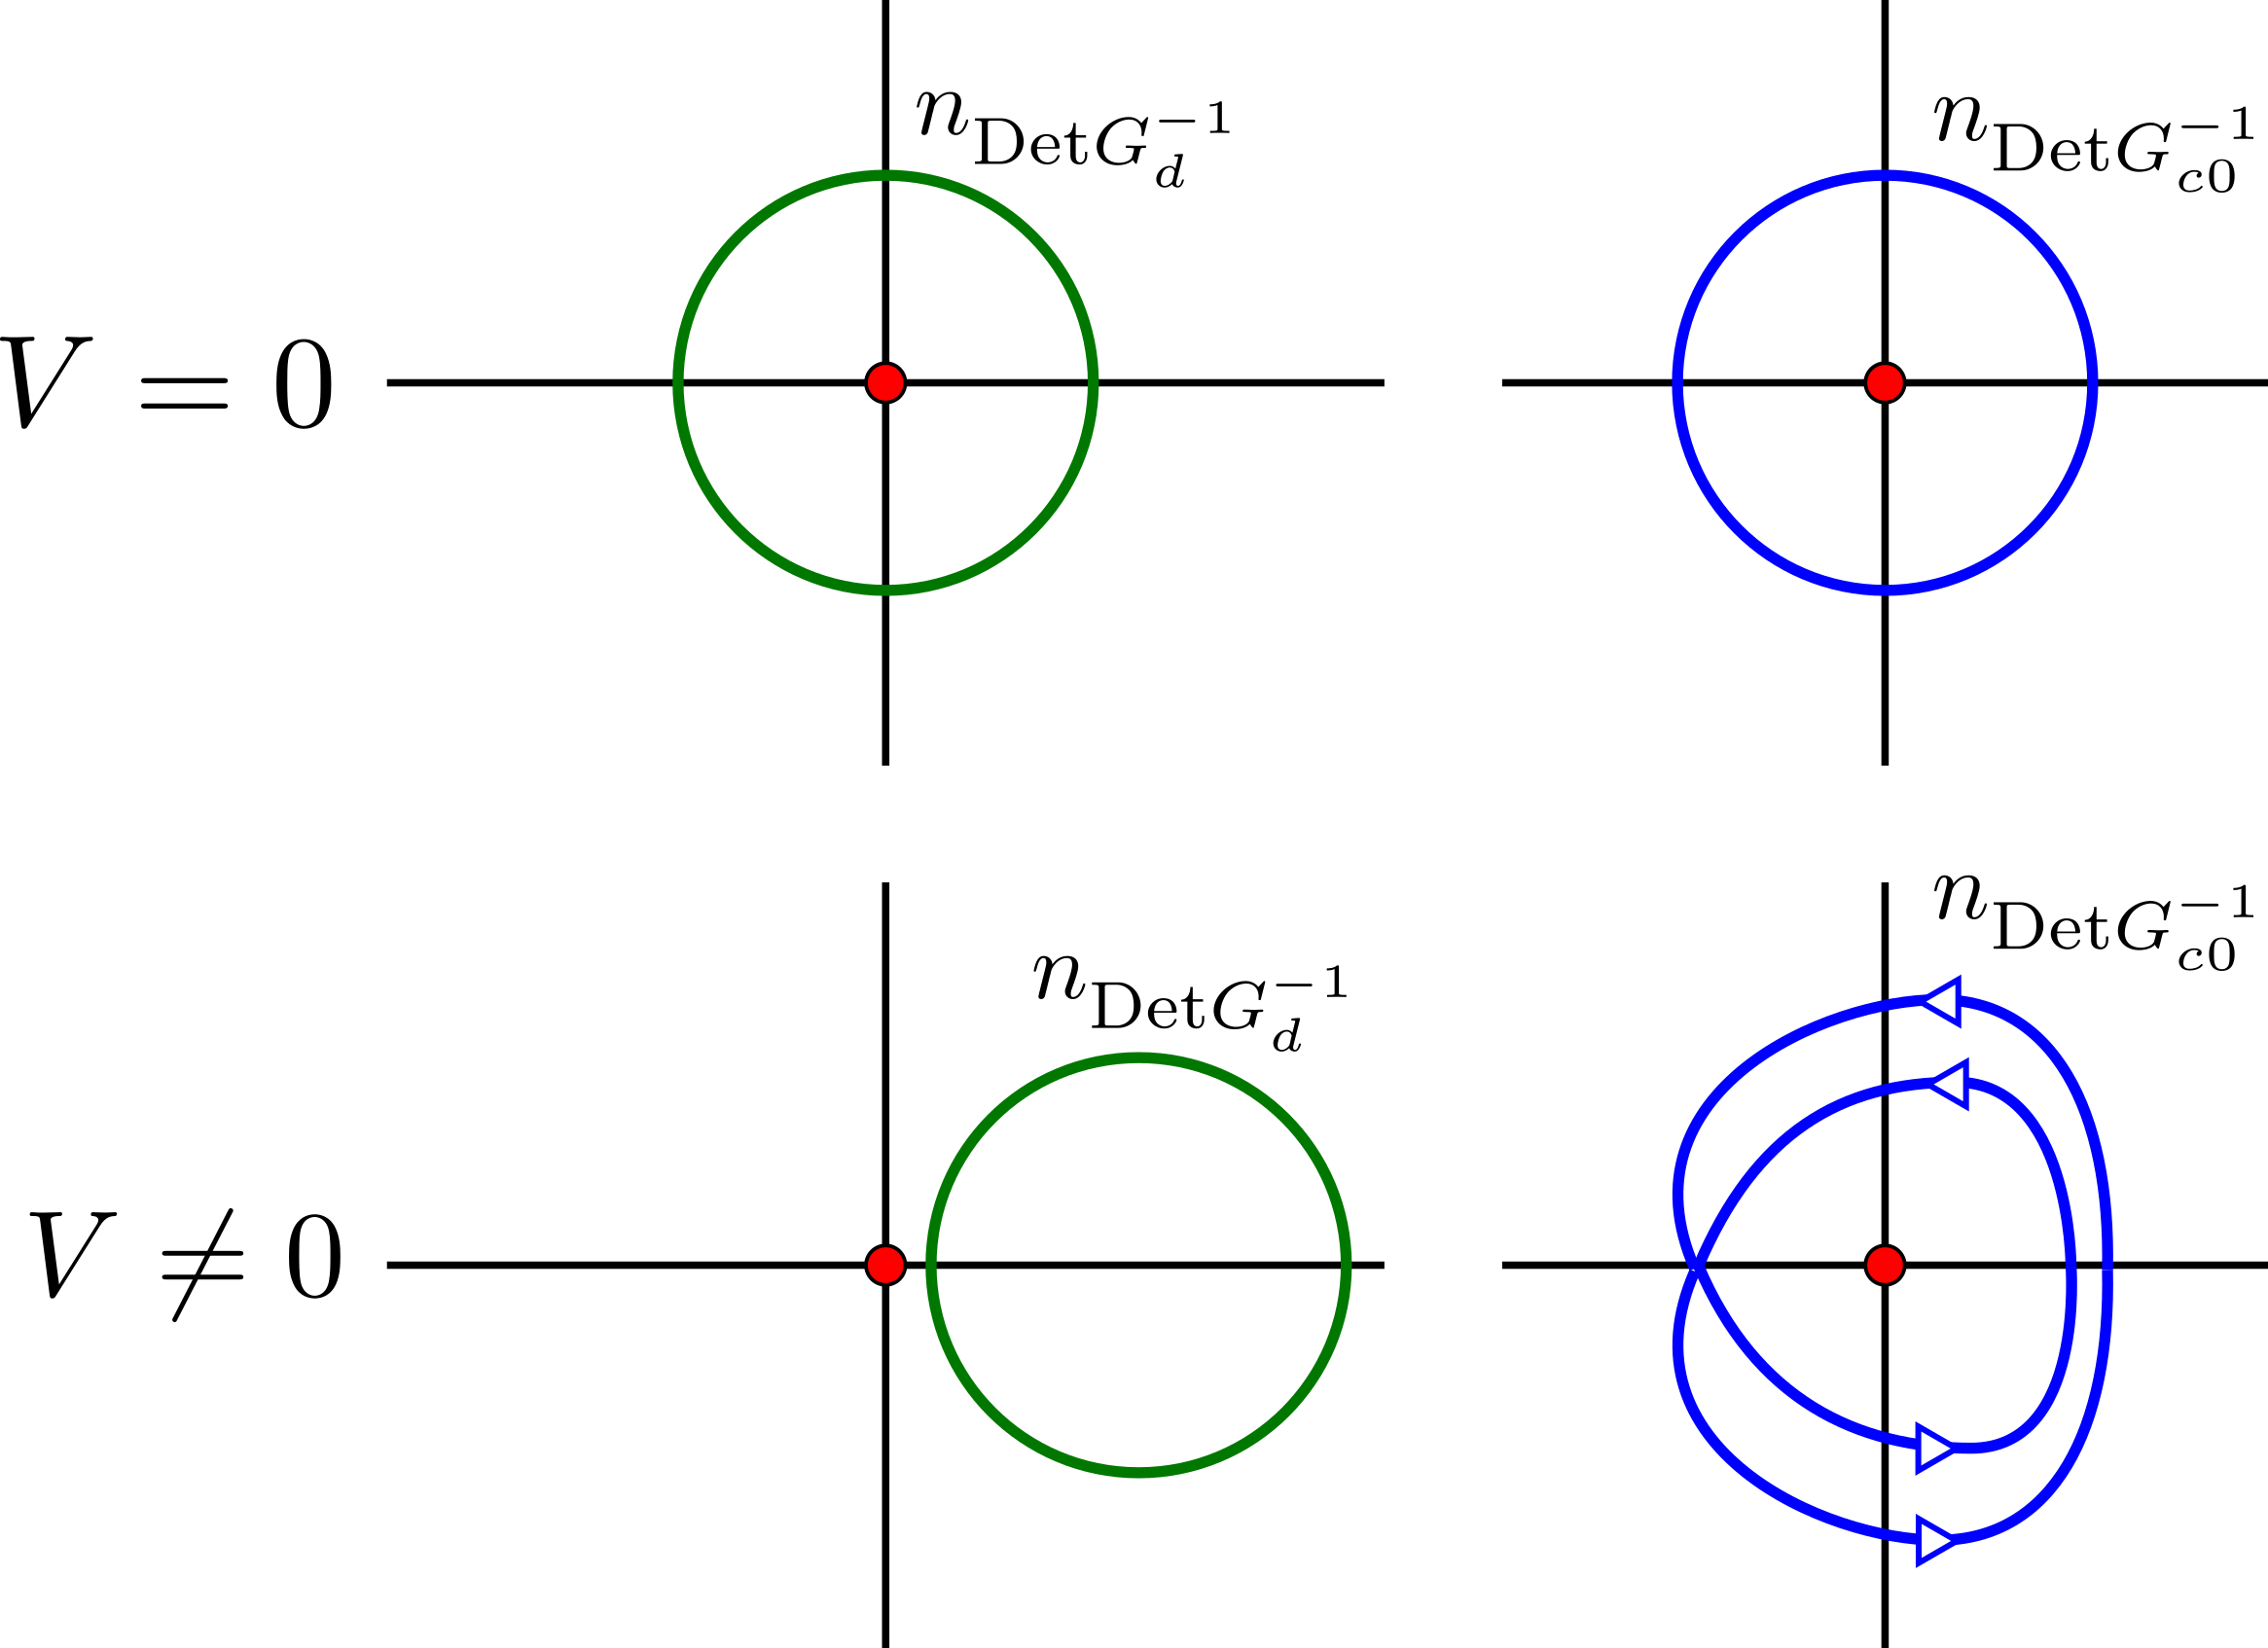
\includegraphics[scale=0.2]{luttinger_top_change.png}
	\caption{The green lines describe the winding number related to the impurity Greens function, while the blue lines do it for the bath. At the local moment fixed point \(V=0\), the impurity has a winding number of 1 because the curve encircles the origin once. At the strong-coupling fixed point, this winding number becomes zero, indicated by the fact that the curve does not encircle the origin even once. The reduction in the winding number on the part of the impurity is directly linked to the increase in the winding number of the bath - it encircles the origin once at the local moment fixed point but twice at strong-coupling.}
	\label{imp_winding}
\end{figure}


\section{Greens function in the insulating phase: the Hubbard bands and mottness}
In the insulating state, the cluster becomes a local moment and the bulk system reduces to the atomic limit \(H = -\frac{U}{2}\sum_i\left(\hat n_{i \uparrow} - \hat n_{i \downarrow}\right)^2\). The Greens function in this limit is given in Appendix~\ref{atomic limit}. From eq.~\ref{atomic_limit_gf}, we have
\begin{equation}\begin{aligned}
	G_{i}(\omega) = \sum_\sigma G_{i,\sigma}(\omega) = \frac{1 + \left<\tau_{i }\right>}{\omega - \frac{U}{2}} + \frac{1 - \left<\tau_{i}\right>}{\omega + \frac{U}{2}}
\end{aligned}\end{equation}
where \(\tau_i = \sum_\sigma \hat n_{i,\sigma} - 1\). At half-filling \(\left<\tau_{i}\right>=0\), the low and high-energy poles have equal spectral weights. \textit{This is different from the situation in a band insulator, where the valence band has all the spectral weight in the ground state while the conduction band is empty.} On doping holes into the system such that \(\left<\tau_{i}\right> = -x < 0\), spectral weight is transferred from the upper Hubbard band at \(\omega = U/2\) to the lower one at \(\omega = -U/2\):

\begin{equation}\begin{aligned}
	G_{i}(\omega) = \sum_\sigma G_{i,\sigma}(\omega) = \frac{1 - x}{\omega - \frac{U}{2}} + \frac{1 + x}{\omega + \frac{U}{2}}
\end{aligned}\end{equation}
\textit{This transfer of spectral weight across energy scales of the order of \(U\), as well as the lack of poles at zero energies, is referred to as mottness}~\cite{phillips2006mottness}.
\begin{figure}[!htb]
	\centering
	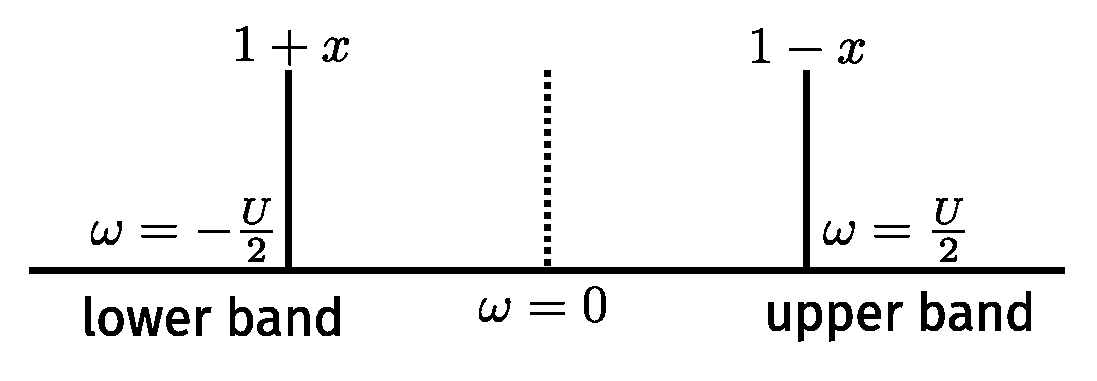
\includegraphics[width=0.5\textwidth]{hubbard_bands.pdf}
	\caption{Structure of the Greens function in the atomic limit. The two poles at \(\omega = \pm \frac{U}{2}\) form the two Hubbard bands. Doping the system leads to transfer of spectral weight between the bands.}
\end{figure}

\section{Nature of propagation: metal vs insulator}
In the metallic state, the impurity in the auxiliary model hybridises with the bath through both 1-particle and 2-particle interactions. For any two auxiliary models differing by the locations \(i_1, i_2\) of the impurity, the baths will always overlap. This means that an electron that starts out from the impurity site at \(i_1\) can hop into the bath, and eventually reach \(i_2\) by hopping out of the other bath and into the other impurity. Such processes connect all sites of the lattice and \textit{allow spectral flow}.

In the insulating state, each auxiliary model separates into an impurity and a bath that decoupled from each other. This means that the impurity cannot hybridise into the bath, and hence cannot tunnel into any other impurity. This leads to the atomic limit of the system, where each site develops a local moment configuration because of the repulsive local correlation, but these local moments cannot communicate with each other, either through spin-exchange processes or by breaking into holons and doublons. Any attempt at spectral flow fails because the boundaries of the system become disconnected from each other.

A more accurate picture of the insulating and metallic phases can be obtained by working with a more complicated choice of the cluster. For instance, instead of a single impurity, one can take two correlated impurities interacting with each other through a single-particle hopping, and this cluster then interacts with the bath through the usual interactions. The ground state of such a cluster is actually a quantum liquid, consisting of the entangled spin and charge degrees of freedom. In the metallic state, various members of this liquid such as the holons, doublons and the spinons are free to propagate across the system through the baths. In the insulating state, it is this cluster that then gets decoupled from the other clusters. The composite degrees of freedom are then unable to propagate outside the cluster, and \textit{the holons and the doublons are bound to each other}~\cite{Mott_1949} within the confines of the cluster.

\begin{figure}[ht]
	\centering
	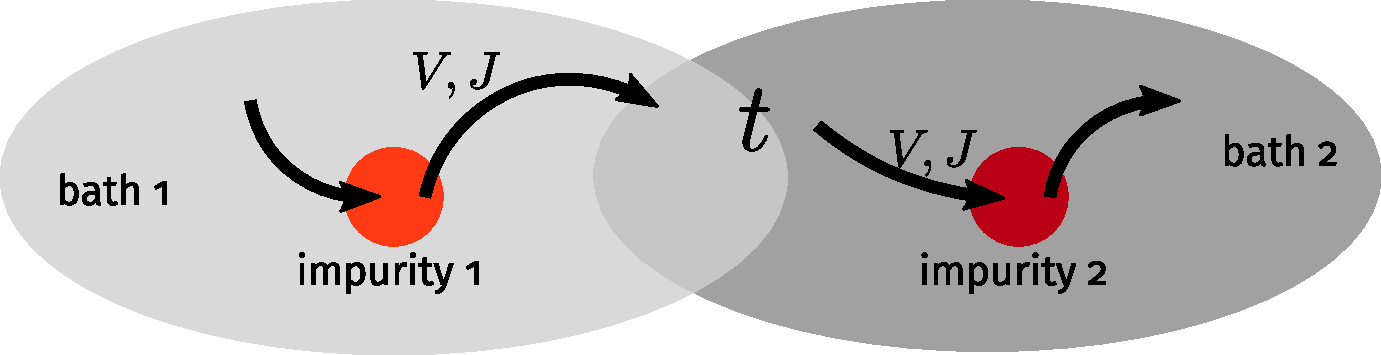
\includegraphics[width=0.55\textwidth]{metal_prop.pdf}
	\caption{Propagation of electrons from one cluster to another through the bath, in the metallic state}
\end{figure}

\begin{figure}[!ht]
	\centering
	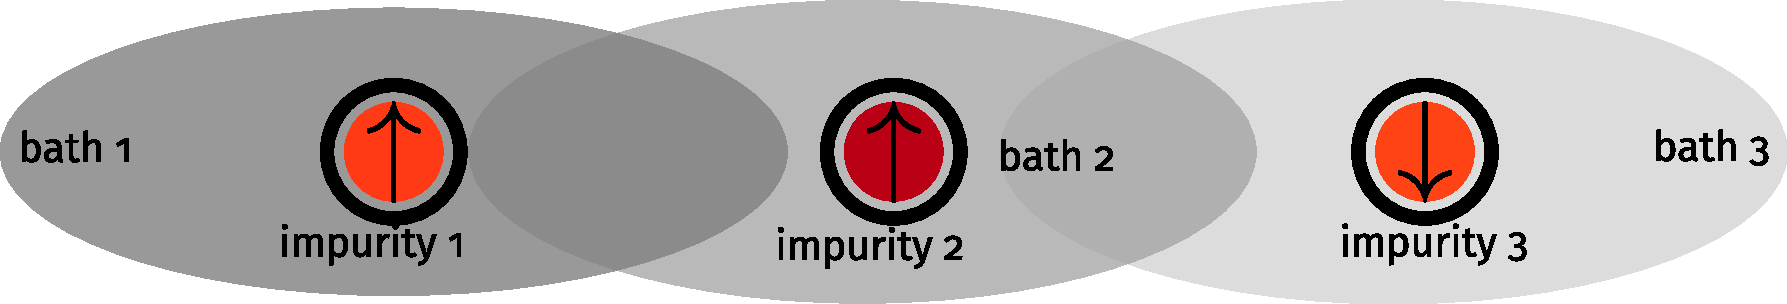
\includegraphics[width=0.75\textwidth]{ins_prop.pdf}
	\caption{The clusters get isolated from each other in the insulator, because they get decoupled from their baths.}
\end{figure}

\begin{figure}[!ht]
	\centering
	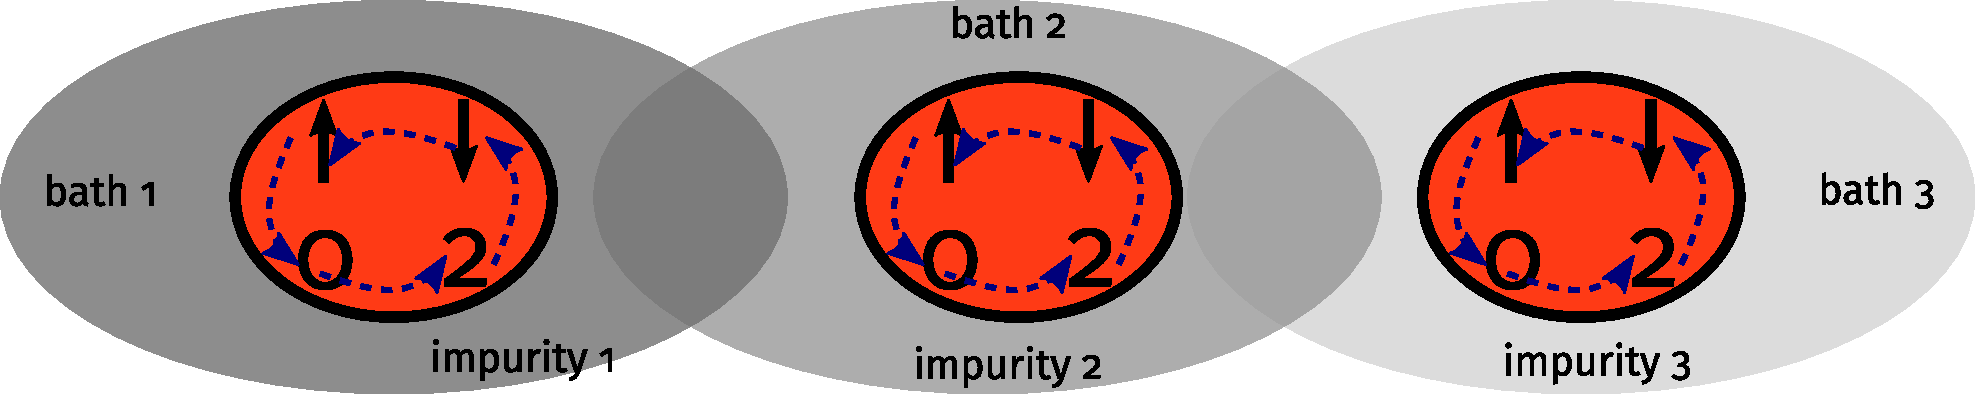
\includegraphics[width=0.85\textwidth]{ins_prop_cluster.pdf}
	\caption{Each cluster is a quantum liquid composed of spin \(\left(\uparrow,\downarrow\right) \) and charge \(\left(0,2\right) \) degrees of freedom. In the insulating state, these degrees of freedom get bound within the cluster and are unable to propagate outside.}
\end{figure}

\section{Presence of two self-energies under symmetry-breaking}
The effective Hamiltonian that describes either the metallic or the insulating phase has $\mathrm{SU}(2)$ symmetry in both the spin and charge sectors. Since the repulsive correlation on the impurity picks out the spin sector, we focus on that for now. Applying a small magnetic field on the impurity breaks this spin-rotation symmetry and picks out either the up or the down state on the impurity, leading to two kinds of self-energies, one for each spin state~\cite{logan_2014,Logan_2015}. The Hamiltonian has the form \(H(h)_i = -\frac{U}{2}\left(\hat n_{i \uparrow} - \hat n_{i \downarrow}\right)^2 - h\left(\hat n_{i \uparrow} - \hat n_{i \downarrow}\right)\). The unique ground-state is \(\ket{\hat n_{i,\sigma = \text{sgn}(h)}=1,\hat n_{i,\sigma = -\text{sgn}(h)}=0}\), with an energy of \(E_\text{gs} = -\frac{U}{2} - h\). The Greens function is easiest to obtain from the Lehmann-Kallen representation (eq.~\ref{Gf_lk}):
\begin{equation}\begin{aligned}
	G_{i,\sigma} = \sum_{n}\left[||\bra{\text{GS}}c_{i\sigma}\ket{n}||^2\frac{1}{\omega + E_\text{GS} - E_n} + ||\bra{n}c_{i\sigma}\ket{\text{GS}}||^2\frac{1}{\omega - E_\text{GS} + E_n}\right]\\
\end{aligned}\end{equation}
We have \(c_{i,\sigma}\ket{\text{GS}} = \ket{\hat n_i = 0}\delta_{\sigma,\text{sgn}(h)}\) and \(c^\dagger_{i,\sigma}\ket{\text{GS}} = \ket{\hat n_i = 2}\delta_{\sigma,-\text{sgn}(h)}\), so that the only excited states that give non-zero inner product is \(\ket{n}=\ket{\hat n_i = 0}\) for the second term and \(\ket{n}=\ket{\hat n_i=2}\) for the first term, with energies \(E_n=0\). Substituting these, we get
\begin{equation}\begin{aligned}
	G_{i,\sigma}(h) = \frac{\delta_{\sigma,-\text{sgn}(h)}}{\omega - \frac{U}{2} - h} + \frac{\delta_{\sigma,\text{sgn}(h)}}{\omega + \frac{U}{2} + h} = \frac{1}{\omega + \left(\frac{U}{2}+h\right)\sigma \times \text{sgn}(h) }
\end{aligned}\end{equation}
Taking the limit of \(h \to 0^\pm\) then gives
\begin{equation}\begin{aligned}
	G_{i,\sigma}(h=0^\pm) = \frac{1}{\omega \pm \frac{U}{2}\sigma}
\end{aligned}\end{equation}
The self-energies arising from the correlation \(U\) can also be obtained using Dyson's equation \(\Sigma = G^{-1} - G_0^{-1}\), where \(G_0^{-1} = \omega\) is the Greens function at \(U=0\). Using Dyson's equation, we get
\begin{equation}\begin{aligned}
	\Sigma_{i,\sigma} = \pm\frac{U}{2}\sigma
\end{aligned}\end{equation}

\section{Analytic consistency check - On the Bethe lattice}
We now apply our approach to the case of infinite number of nearest-neighbours $\mathcal{W}\to\infty$ (the coordination number, and effectively the dimension). In such a model, the correct scaling of the $t^{H}$ hopping parameter is $t^{H}\to t^{H}/\sqrt{\mathcal{W}}$~\cite{metzner_volhardt_1989,georges_kotliar_1992,pruschke_cox_jarrel_1993}, such that the kinetic energy of the associated tight-binding lattice model remains finite and in competition with the localising physics of \(U\) and the magnetic ordering physics of \(J\). This allows a metal-insulator transition in the limit of $\mathcal{W}\to\infty$ as well. In this limit, the dependence of the self-energy on the interacting Greens function can be shown to arise from only the site-diagonal terms~\cite{Muller-Hartmann1989,georges_kotliar_1992}. This can be demonstrated from the present formalism as well, using eq.\eqref{self-energy1}. Applying the limit of \(w\to \infty\) on that equation gives
\begin{equation}\begin{aligned}
	\Sigma_{H-H}(\vec k,\omega) = \lim_{w\to \infty} \left\{\left(G^{(0)}(\vec k,\omega)\right)^{-1} - \left [G_\text{aux,dd} + \frac{\xi_{\vec k}}{\mathcal{W}} G_\text{aux,dz}\right]^{-1}\right\} = \lim_{w\to \infty}\left\{G^{(0)}(\vec k,\omega) - G_\text{aux,dd}(\omega)\right\}^{-1} 
\end{aligned}\end{equation}
where \(G^{(0)}(\vec k,\omega)\) is the non-interacting Greens function and \(G_\text{aux,dd}(\omega)\) is the site-diagonal Greens function of the auxiliary model. It is clear from the final form that only the diagonal term \(G_\text{aux,dd}(\omega)\) of the interacting Greens function affects the self-energy while the off-diagonal part \(G_\text{aux,dz}\) fails to contribute as \(w \to \infty\). 
\par
\textbf{MAKE CONNECTION BETWEEN COM and Q.IMP PROBLEM}
\begin{appendices}

\appendixtitleon

\chapter{Zero temperature Greens function in frequency domain}

\label{appx-spectral-func}
The impurity retarded Green's function (assuming the Hamiltonian to be time-independent, which it is) is defined as
\begin{equation}\begin{aligned}
	G_{dd}^\sigma(t) = -i\theta(t) \left<\left\{ \mathcal{O}_{\sigma}(t),\mathcal{O}^\dagger_{\sigma} \right\}  \right>
\end{aligned}\end{equation}
where the average \(\left< \right>\) is over a canonical ensemble at temperature \(T\), and \(\mathcal{O}_\sigma = c_{d\sigma} + S_d^- c_{0\overline\sigma} + S_d^z c_{0\sigma}\) is the excitation whose spectral function we are interested in. The excitations defined in \(\mathcal{O}\) incorporates both single-particle excitations brought about by the hybridisation as well as two-particle spin excitations brought about by the spin-exchange term. What follows is a standard calculation where we write the Green's function in the Lehmann-Kallen representation. The ensemble average for an arbitrary operator \(\hat M\) can be written in terms of the exact eigenstates of the fixed point Hamiltonian:
\begin{equation}\begin{aligned}
	H^* \ket{n} &= E_n^* \ket{n}, ~ ~ ~\left<\hat M \right> &\equiv \frac{1}{Z}\sum_n \bra{n} \hat M \ket{n} e^{-\beta E_n^*}
\end{aligned}\end{equation}
where \(Z = \sum_n e^{-\beta E_n^*}\) is the fixed point partition function and \(\left\{ \ket{n} \right\} \) is the set of eigenfunctions of the fixed point Hamiltonian. We can therefore write
\begin{equation}\begin{aligned}
	&\left<\left\{ \mathcal{O}_{\sigma}(t),\mathcal{O}^\dagger_{\sigma} \right\}  \right> \\
	&= \frac{1}{Z}\sum_{m}e^{-\beta E_m}\bra{m}\left\{ \mathcal{O}_{\sigma}(t),\mathcal{O}^\dagger_{\sigma} \right\} \ket{m}\\
	&= \frac{1}{Z}\sum_{m,n}e^{-\beta E_m}\bra{m}\left( \mathcal{O}_{\sigma}(t)\ket{n}\bra{n}\mathcal{O}^\dagger_{\sigma} + \mathcal{O}^\dagger_{\sigma}\ket{n}\bra{n}\mathcal{O}_{\sigma}(t)\right) \ket{m} && \left[\sum_n \ket{n}\bra{n} = 1\right]  \\
	&= \frac{1}{Z}\sum_{m,n}e^{-\beta E_m}\bra{m}\left( e^{iH^* t}\mathcal{O}_{\sigma}e^{-iH^* t}\ket{n}\bra{n}\mathcal{O}^\dagger_{\sigma} + \mathcal{O}^\dagger_{\sigma}\ket{n}\bra{n}e^{iH^* t}\mathcal{O}_{\sigma}e^{-iH^* t}\right) \ket{m}\\
	&= \frac{1}{Z}\sum_{m,n}e^{-\beta E_m}\left( e^{i\left( E_m - E_n \right)  t}\bra{m}\mathcal{O}_{\sigma}\ket{n}\bra{n}\mathcal{O}^\dagger_{\sigma} \ket{m} + e^{i\left( E_n - E_m \right)  t}\bra{m}\mathcal{O}^\dagger_{\sigma}\ket{n}\bra{n}\mathcal{O}_{\sigma} \ket{m}\right)\\
	&= \frac{1}{Z}\sum_{m,n}e^{i\left( E_m - E_n \right)  t}||\bra{m}\mathcal{O}_{\sigma}\ket{n}||^2\left( e^{-\beta E_m} + e^{-\beta E_n}\right)\\
\end{aligned}\end{equation}
The time-domain impurity Green's function can thus be written as (this is the so-called Lehmann-Kallen representation)
\begin{equation}\begin{aligned}
	G_{dd}^\sigma = -i\theta(t)\frac{1}{Z}\sum_{m,n}e^{i\left( E_m - E_n \right)  t}||\bra{m}\mathcal{O}_{\sigma}\ket{n}||^2\left( e^{-\beta E_m} + e^{-\beta E_n}\right)\\
\end{aligned}\end{equation}
We are interested in the frequency domain form.
\begin{equation}\begin{aligned}
	G_{d d}^\sigma(\omega) &= \int_{-\infty}^\infty dt e^{i \omega t}G_{d d}^\sigma(t) \\
			       &= \frac{1}{Z}\sum_{m,n}||\bra{m}\mathcal{O}_{\sigma}\ket{n}||^2\left( e^{-\beta E_m} + e^{-\beta E_n}\right)\left(-i\right)\int_{-\infty}^\infty dt \theta(t)e^{i\left( \omega + E_m - E_n \right)t}
\end{aligned}\end{equation}
To evaluate the time-integral, we will use the integral representation of the Heaviside function:
\begin{equation}\begin{aligned}
	\theta(t) = \frac{1}{2\pi i}\lim_{\eta \to 0^+} \int_{-\infty}^\infty \frac{1}{x- i\eta}e^{ixt}dx
\end{aligned}\end{equation}
With this definition, the integral in \(G_{dd}^\sigma(\omega)\) becomes
\begin{equation}\begin{aligned}
	\left(-i\right)\int_{-\infty}^\infty dt \theta(t)e^{i\left( \omega + E_m - E_n \right)t} &= \left(-i\right)\frac{1}{2\pi i}\lim_{\eta \to 0^+} \int_{-\infty}^\infty dx\frac{1}{x- i\eta}\int_{-\infty}^\infty dt e^{i\left( \omega + E_m - E_n + x\right)t} \\
									     &=\left(-i\right)\frac{1}{2\pi i}\lim_{\eta \to 0^+} \int_{-\infty}^\infty dx\frac{1}{x- i\eta} 2\pi \delta\left( \omega + E_m - E_n + x\right) \\
									     &=\left(-i\right)\frac{1}{i}\lim_{\eta \to 0^+} \frac{-1}{\omega + E_m - E_n- i\eta} \\
									     &=\frac{1}{\omega + E_m - E_n} \\
\end{aligned}\end{equation}
The frequency-domain Green's function is thus
\begin{equation}\begin{aligned}
	G_{d d}^\sigma(\omega) = \frac{1}{Z}\sum_{m,n}||\bra{m}\mathcal{O}_{\sigma}\ket{n}||^2\left( e^{-\beta E_m} + e^{-\beta E_n}\right)\frac{1}{\omega + E_m - E_n}
\end{aligned}\end{equation}
The zero temperature Green's function is obtained by taking the limit of \(\beta \to \infty\). In both the partition function as well as inside the summation, the only term that will survive is the exponential of the ground state energy \(E_0\).
\begin{equation*}\begin{aligned}
	Z \equiv \sum_m e^{-\beta E_m} \implies \lim_{\beta \to \infty}Z = d_0 e^{-\beta E_0}, && E_0 \equiv \text{min}\left\{ E_n \right\} 
\end{aligned}\end{equation*}
where \(d_0\) is the degeneracy of the ground state. The Greens function then simplifies to
\begin{equation}\begin{aligned}
	\label{Gf_lk}
	G_{d d}^\sigma(\omega, \beta \to \infty) &= \frac{1}{d_0e^{-\beta E_0}}\sum_{m,n}||\bra{m}\mathcal{O}_{\sigma}\ket{n}||^2\left[e^{-\beta E_m}\delta_{E_m, E_0} + e^{-\beta E_n}\delta_{E_n, E_0}\right]\frac{1}{\omega + E_m - E_n}\\
						 &= \frac{1}{d_0}\sum_{n,0}\left[||\bra{0}\mathcal{O}_{\sigma}\ket{n}||^2\frac{1}{\omega + E_0 - E_n} + ||\bra{n}\mathcal{O}_{\sigma}\ket{0}||^2\frac{1}{\omega - E_0 + E_n}\right]\\
\end{aligned}\end{equation}
The label 0 sums over all states \(\ket{0}\) with energy \(E_0\). The spectral function is the imaginary part of this Green's function. To extract the imaginary part, we insert an infinitesimal imaginary part in the denominator:
\begin{equation}\begin{aligned}
	G_{d d}^\sigma(\omega, \eta) = \frac{1}{d_0}\lim_{\eta \to 0^-}\sum_{n,0}\left[||\bra{0}\mathcal{O}_{\sigma}\ket{n}||^2\frac{1}{\omega + E_0 - E_n + i\eta} + ||\bra{n}\mathcal{O}_{\sigma}\ket{0}||^2\frac{1}{\omega - E_0 + E_n + i\eta}\right]\\
\end{aligned}\end{equation}
The spectral function at zero temperature can then be written as
\begin{equation}\begin{aligned}
	\mathcal{A(\omega)} &= -\frac{1}{\pi}\text{ Im }\left[G_{dd}^\sigma\left( \omega \right) \right] \\
			    &= \frac{1}{d_0}\frac{1}{\pi}\text{ Im }\left[\lim_{\eta \to 0^-}\sum_{n,0}\left(\frac{-i\eta ||\bra{0}\mathcal{O}_{\sigma}\ket{n}||^2}{\left(\omega + E_0 - E_n\right)^2 + \eta^2} + \frac{-i\eta ||\bra{n}\mathcal{O}_{\sigma}\ket{0}||^2}{\left(\omega - E_0 + E_n\right)^2 + \eta^2}\right)\right]\\
			    &= \frac{1}{d_0}\frac{1}{\pi}\sum_{n,0}\left[||\bra{0}\mathcal{O}_{\sigma}\ket{n}||^2\pi\delta\left(\omega + E_0 - E_n\right) + ||\bra{n}\mathcal{O}_{\sigma}\ket{0}||^2\pi\delta\left(\omega - E_0 + E_n\right)\right]\\
			    &= \frac{1}{d_0}\sum_{n,0}\left[||\bra{0}\mathcal{O}_{\sigma}\ket{n}||^2\delta\left(\omega + E_0 - E_n\right) + ||\bra{n}\mathcal{O}_{\sigma}\ket{0}||^2\delta\left(\omega - E_0 + E_n\right)\right]\\
\end{aligned}\end{equation}

\chapter{Some analytic results for the Hubbard dimer and the Hubbard model}
\section{Spectrum of the Hubbard dimer}
Here we document the spectrum of the Hubbard dimer Hamiltonian.
\begin{center}
	\begin{tabular}{|c|c|c|}
	\hline
	eigenstate & symbol & eigenvalue \\
	\hline
	$\ket{0,0}$ & $\ket{0}$ & \( \frac{U^H}{2}\)\\
	$ \frac{1}{\sqrt 2}\left(\ket{\sigma,0} \pm \ket{0,\sigma}\right)$ & $\ket{0\sigma_\pm}$ & \(\mp t^H\)\\
	$\ket{\sigma,\sigma}$ & $\ket{\sigma\sigma}$ & \( -\frac{U^H}{2}\)\\
	$ \frac{1}{\sqrt 2}\left(\ket{\uparrow,\downarrow} + \ket{\downarrow,\uparrow}\right)$ & $\ket{ST}$ & \( -\frac{U^H}{2}\)\\
	$ \frac{1}{\sqrt 2}\left(\ket{2,0} - \ket{0,2}\right)$ & $\ket{CS}$ & \( \frac{U^H}{2}\)\\
	$a_1(U^H, t^H) \frac{1}{\sqrt 2}\left(\ket{\uparrow,\downarrow} - \ket{\downarrow,\uparrow}\right) + a_2(U^H, t^H)\frac{1}{\sqrt 2}\left(\ket{2,0} + \ket{0,2}\right)$ & $\ket{-}$ & \(-\frac{1}{2}\Delta(U^H, t^H)\)\\
	$-a_2(U^H, t^H) \frac{1}{\sqrt 2}\left(\ket{\uparrow,\downarrow} - \ket{\downarrow,\uparrow}\right) + a_1(U^H, t^H)\frac{1}{\sqrt 2}\left(\ket{2,0} + \ket{0,2}\right)$ & $\ket{+}$ & \(\frac{1}{2}\Delta(U^H, t^H)\)\\
	$ \frac{1}{\sqrt 2}\left(\ket{\sigma,2} \pm \ket{2,\sigma}\right)$ & $\ket{2\sigma_\pm}$ & \(\pm t^H\)\\
	$\ket{2,2}$ & $\ket{4}$ & \( \frac{U^H}{2}\)\\
\hline
	\end{tabular}
	\captionof{table}{Spectrum of Hubbard dimer at half-filling}
	\label{hubb_dim_spectrum}
\end{center}

\section{Greens function of Hubbard model in the atomic limit}
\label{atomic limit}
The atomic limit is described by the Hamiltonian \(H = -\frac{U}{2}\sum_i\left(\hat n_{i \uparrow} - \hat n_{i \downarrow}\right)^2\). Since the Hamiltonian has decoupled into \(\sum_i \equiv N\) single-site Hamiltonians, we can easily write down the retarded Greens function for a single site by identifying the ground state configuration of a site. The ground states are of course \(\ket{\Psi}_i = \ket{\uparrow},\ket{\downarrow}\), in the absence of any symmetry-breaking. The finite temperature retarded Greens function in the time domain is given by
\begin{equation}\begin{aligned}
	G_{i,\sigma}(T,t) = -i\theta(t) \frac{1}{Z}\sum_n e^{-\beta E_n} \braket{n | \left\{c_{i\sigma}(t),c^\dagger_{i\sigma}\right\} | n}
\end{aligned}\end{equation}
where \(n\) labels the eigenstates of the \(H\). At \(T \to 0\), only the ground states will survive in the exponential and the partition function \(Z\), such that the formula then reduces to
\begin{equation}\begin{aligned}
G_{i,\sigma}(T \to 0,t) = -i\theta(t)\braket{GS | \left\{c_{i\sigma}(t),c^\dagger_{i\sigma}\right\} | GS}
\end{aligned}\end{equation}
Since the Hamiltonian is simple, we can compute the time-dependent operator \(c_{i\sigma}(t) = e^{iH t} c_{i\sigma} e^{-iHt}\). Using the BCH lemma, we have
\begin{equation}\begin{aligned}
	e^{iH t} c_{i\sigma} e^{-iHt} = \sum_{n=0}^\infty \left(it\right)^n \frac{1}{n!}\left[H,c_{i\sigma}\right]_n
\end{aligned}\end{equation}
where \(\left[H,c_{i\sigma}\right]_n = \left[H,\left[H,c_{i\sigma}\right]_{n-1}\right],\left[H,c_{i\sigma}\right]_0=c_{i\sigma}\). The first two non-trivial commutators are
\begin{equation}\begin{aligned}
	\left[H, c_{i\sigma}\right]_1 = -U \tau_{i\overline\sigma}c_{i\sigma},~ ~\text{and} ~~\left[H, c_{i\sigma}\right]_2 = \frac{1}{4}U^2 c_{i\sigma}~,
\end{aligned}\end{equation}
such that
\begin{equation}\begin{aligned}
	e^{iH t} c_{i\sigma} e^{-iHt} =& \left[c_{i\sigma} + \frac{i^2 t^2}{2!}\frac{U^2}{2^2} c_{i\sigma} + \frac{i^4 t^4}{4!}\frac{U^4}{2^4} c_{i\sigma} + \ldots\right] + \left[- \frac{it}{1!}U\tau_{i\overline\sigma}c_{i\sigma} - \frac{i^3 t^3}{3!}\frac{U^3}{4}\tau_{i\overline\sigma}c_{i\sigma} + \ldots \right]\\
				       &= c_{i\sigma} \left[\cos\left(Ut/2\right) - 2i\tau_{i\overline\sigma}\sin \left(Ut/2\right) \right] 
\end{aligned}\end{equation}
Using this, we can write
\begin{equation}\begin{aligned}
	\left\{c_{i\sigma}(t),c^\dagger_{i\sigma}\right\} = \left\{c_{i\sigma},c^\dagger_{i\sigma}\right\} \left[\cos\left(Ut/2\right) - 2i\tau_{i\overline\sigma}\sin \left(Ut/2\right) \right] = \left[\cos\left(Ut/2\right) - 2i\tau_{i\overline\sigma}\sin \left(Ut/2\right) \right]
\end{aligned}\end{equation}
and the Greens function becomes
\begin{equation}\begin{aligned}
	G_{i,\sigma}(T \to 0,t) = -i\theta(t) \braket{GS | \left[\cos\left(Ut/2\right) - 2i\tau_{i\overline\sigma}\sin \left(Ut/2\right) \right] | GS} = -i\theta(t)\left[\cos \frac{Ut}{2} - 2i\sin \frac{Ut}{2} \left<\tau_{i\overline\sigma} \right>\right]
\end{aligned}\end{equation}
We now Fourier transform to frequency domain:
\begin{equation}\begin{aligned}
	G_{i,\sigma}(\omega) = -i\int_{0}^\infty \mathrm{dt} e^{i\omega t}\left[\cos \frac{Ut}{2} - 2i\sin \frac{Ut}{2} \left<\tau_{i\overline\sigma} \right>\right] = \frac{1 + \left<\tau_{i\overline\sigma }\right>}{\omega - \frac{U}{2}} + \frac{1 - \left<\tau_{i\overline\sigma}\right>}{\omega + \frac{U}{2}}
\end{aligned}\end{equation}
The spin-total Greens function for the site \(i\) is
\begin{equation}\begin{aligned}
	\label{atomic_limit_gf}
	G_{i}(\omega) = \sum_\sigma G_{i,\sigma}(\omega) = \frac{1 + \left<\tau_{i }\right>}{\omega - \frac{U}{2}} + \frac{1 - \left<\tau_{i}\right>}{\omega + \frac{U}{2}}
\end{aligned}\end{equation}
At half-filling, we have \(\tau_i = 1\).
\section{Local Greens function for the Hubbard dimer}
From the spectral representation, we have the following expression for the local Greens function for the Hubbard dimer at site $0$:
\begin{equation}\begin{aligned}
	G_{D,00}^\sigma(\omega) = \frac{1}{Z}\sum_{m,n}||\bra{m}c_{i\sigma}\ket{n}||^2\left( e^{-\beta E_m} + e^{-\beta E_n}\right)\frac{1}{\omega + E_m - E_n}
\end{aligned}\end{equation}
$m,n$ sum over the exact eigenstates. $E_m, E_n$ are the corresponding energies. We are interested in teh $T \to 0$ Greens function. In that limit, all exponentials except that for the ground state $E_{gs}$ will die out. The exponential inside the summation will then cancel the exponential in the partition function.
\begin{equation}\begin{aligned}
	G_{D,00}^\sigma(\omega, T \to 0) &= \sum_{n}\left[||\bra{GS}c_{i\sigma}\ket{n}||^2\frac{1}{\omega + E_{GS} - E_n} + ||\bra{n}c_{i\sigma}\ket{GS}||^2\frac{1}{\omega + E_n - E_{GS}}\right]\\
					&= \sum_{n}\left[||\bra{n}c^\dagger_{i\sigma}\ket{GS}||^2\frac{1}{\omega + E_{GS} - E_n} + ||\bra{n}c_{i\sigma}\ket{GS}||^2\frac{1}{\omega + E_n - E_{GS}}\right]\\
\end{aligned}\end{equation}

The ground state $\ket{GS}$ is just the state $\ket{-}$ in the table \ref{hubb_dim_spectrum}. We will choose to look at $\sigma = \uparrow`$. Then,
\begin{equation}\begin{aligned}
	c_{1\uparrow}\ket{-} &= \frac{a_1}{\sqrt 2}\ket{0, \downarrow} + \frac{a_2}{\sqrt 2}\ket{\downarrow,0}\\
	c^\dagger_{1\uparrow}\ket{-} &= -\frac{a_1}{\sqrt 2}\ket{2, \uparrow} + \frac{a_2}{\sqrt 2}\ket{\uparrow,2}\\
\end{aligned}\end{equation}
The set of states $\ket{n}$ that give non-zero inner product $\ket{GS}$ are therefore
\begin{equation}\begin{aligned}
	\left\{ \ket{n} \right\} &= \ket{0\downarrow_\pm}\\
	||\bra{n}c_{\uparrow\sigma}\ket{GS}||^2 &= \frac{1}{4}\left(a_2 \pm a_1 \right)^2 = \frac{1}{4}\left(1 \pm 2a_1a_2\right)\\
	\left\{ E_n \right\} &= \mp t
\end{aligned}\end{equation}
for the second inner product, and
\begin{equation}\begin{aligned}
	\left\{\ket{n}\right\} &= \ket{2\uparrow_\pm}\\
	||\bra{n}c^\dagger_{\uparrow\sigma}\ket{GS}||^2 &= \frac{1}{4}\left( a_2 \mp a_1 \right)^2 = \frac{1}{4}\left(1 \mp 2a_1a_2\right)\\
	\left\{ E_n \right\} &= \pm t
\end{aligned}\end{equation}
for the first. The Greens function is therefore
\begin{equation}\begin{aligned}
	\label{dimer_local_G}
	G_{D,00}^\uparrow(\omega, T \to 0) &= \left( \frac{1}{2} + \frac{2t}{\Delta} \right) \frac{\omega}{\omega^2 - \left(t - \frac{\Delta}{2}\right) ^2} + \left( \frac{1}{2} - \frac{2t}{\Delta} \right) \frac{\omega}{\omega^2 - \left(t + \frac{\Delta}{2}\right) ^2} = G_{D,00}^\downarrow(\omega, T \to 0)~.
\end{aligned}\end{equation}
In the atomic limit $(t=0)$, the Greens function simplifies to
\begin{equation}\begin{aligned}
	G_{D,00}^\uparrow(\omega, T \to 0) \bigg\vert_\text{atomic} = \frac{\omega}{\omega^2 - \frac{1}{4}U^2}
\end{aligned}\end{equation}
In the atomic limit, the singly-occupied state has zero energy:
\begin{equation}\begin{aligned}
	E_1(t=0) = \bra{1,0}\left(U \tau_{0 \uparrow}\tau_{0 \downarrow} + U \tau_{1 \uparrow}\tau_{1 \downarrow}\right) \ket{1,0} = 0
\end{aligned}\end{equation}
We can write the atomic limit Greens function in terms of this energy and the self energy:
\begin{equation}\begin{aligned}
	G_{D,00}^\uparrow(\omega, T \to 0) \bigg\vert_\text{atomic} = \frac{1}{\omega - E_1(t=0) - \Sigma(t=0)} = \frac{1}{\omega - 0 -\frac{U^2}{4\omega}}
\end{aligned}\end{equation}
The self energy in the atomic limit can be read off as 
\begin{equation}\begin{aligned}
	\label{dimer_selfenergy}
\Sigma(t=0) = \frac{U^2}{4\omega}
\end{aligned}\end{equation}
The site local spectral function can also be calculated from the local Greens function:
\begin{eqnarray}
A(0\uparrow, \omega) &=& - \frac{1}{\pi}\text{Im }G_{D,00}^\uparrow(\omega)\nonumber\\
			     &=& \left( \frac{1}{4} - \frac{t}{\Delta} \right)\left[\delta(\omega - \frac{1}{2}\Delta - t) + \delta(\omega + \frac{1}{2}\Delta + t)\right]\nonumber\\ 
			     &&+ \left( \frac{1}{4} + \frac{t}{\Delta} \right) \left[\delta(\omega - \frac{1}{2}\Delta + t) + \delta(\omega + \frac{1}{2}\Delta - t)\right]\\ 
			     &=& A(0\downarrow, \omega)~.\nonumber
\end{eqnarray}
Finally, the inter-site Greens function for the Hubbard dimer is given by
\begin{equation}
\label{dimer_intersite_G}
G_{D,01}^\uparrow(\omega, T \to 0) = \left( \frac{1}{2} + \frac{2t}{\Delta} \right) \frac{t - \frac{\Delta}{2}}{\omega^2 - \left(t - \frac{\Delta}{2}\right)^2} + \left( \frac{1}{2} - \frac{2t}{\Delta} \right) \frac{t + \frac{\Delta}{2}}{\omega^2 - \left(t + \frac{\Delta}{2}\right)^2} = G_{D,01}^\downarrow(\omega, T \to 0)~.
\end{equation}
Using the diagonal and off-diagonal real space Greens functions, we can now compute the momentum-space Greens functions. The two momentum states are $ka = 0, \pi$. By Fourier transforming, these two Greens functions can be written as
\begin{equation}\begin{aligned}
	\label{Gk0}
	G(k=0, \sigma) = \sum_r e^{ikr} G(r, \sigma) = G(r=0, \sigma) + G(r=a, \sigma) = \frac{1/2 + 2t/\Delta}{\omega -t + \Delta/2} + \frac{1/2 - 2t/\Delta}{\omega - t - \Delta/2}\\
	G(k=\pi, \sigma) = \sum_r e^{ikr} G(r, \sigma) = G(r=0, \sigma) - G(r=a, \sigma) = \frac{1/2 + 2t/\Delta}{\omega + t - \Delta/2} + \frac{1/2 - 2t/\Delta}{\omega + t + \Delta/2}\\
\end{aligned}\end{equation}

\section{Contributions of various excitations to the site local spectral function}
The site local spectral function is
\begin{equation}\begin{aligned}
	A(0\uparrow, \omega) = \left( \frac{1}{4} - \frac{t}{\Delta} \right)\left[\delta(\omega - \frac{\Delta}{2} - t) + \delta(\omega + \frac{\Delta}{2} + t)\right]\nonumber + \left( \frac{1}{4} + \frac{t}{\Delta} \right) \left[\delta(\omega - \frac{\Delta}{2} + t) + \delta(\omega + \frac{\Delta}{2} - t)\right]
\end{aligned}\end{equation}
If the eigenstates of the $N=1, S^z = - \frac{1}{2}$ sector are $\ket{1 \pm \downarrow}$ and those of $N=3, S^z = \frac{1}{2}$ sector are $\ket{3 \pm \uparrow}$, this spectral function originates from the expression:
\begin{equation}\begin{aligned}
	A(0\uparrow, \omega) =& \braket{1 \downarrow_- | c_{0 \uparrow} | \text{GS}} \delta\left(\omega + \frac{\Delta}{2} + t\right) + \braket{2 \uparrow_+ | c^\dagger_{0 \uparrow} | \text{GS}}\delta\left(\omega - \frac{\Delta}{2} - t\right) \\
			      &+ \braket{1 \downarrow_+ | c_{0 \uparrow} | \text{GS}}\delta\left(\omega + \frac{\Delta}{2} - t\right) + \braket{2 \uparrow_- | c^\dagger_{0 \uparrow} | \text{GS}}\delta(\omega - \frac{\Delta}{2} + t)
\end{aligned}\end{equation}
\begin{figure}[!htb]
	\centering
	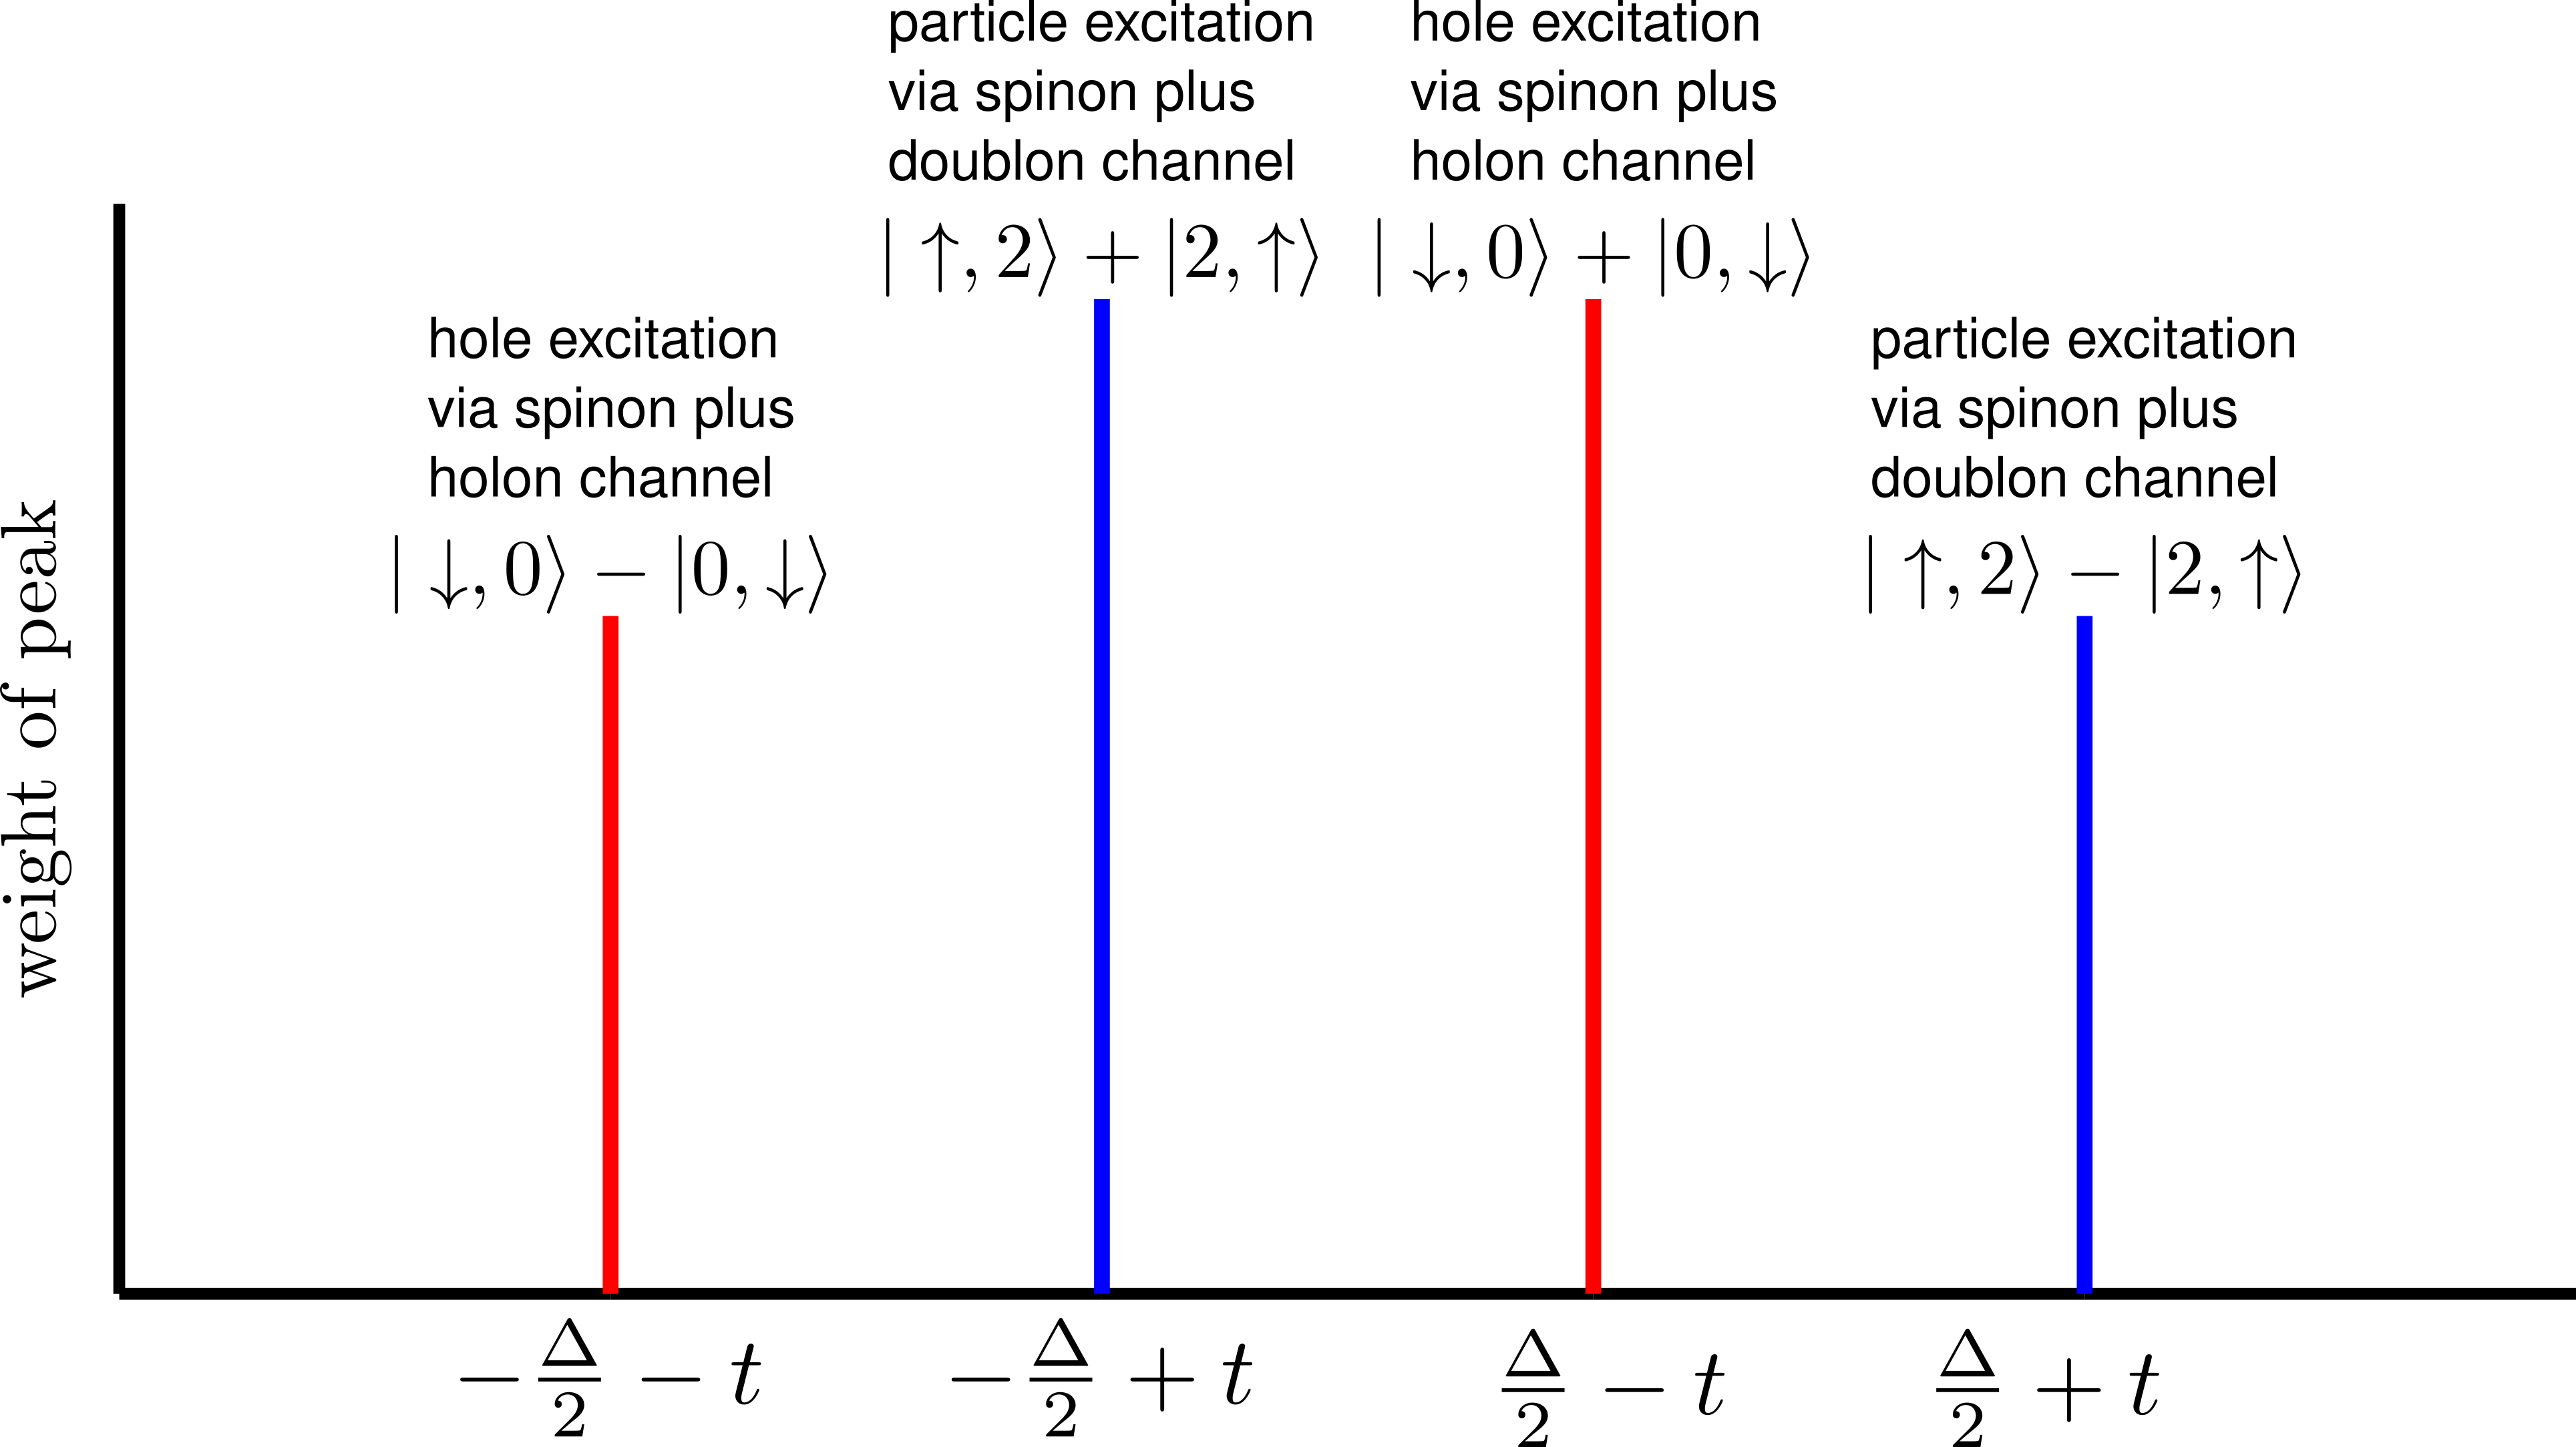
\includegraphics[width=0.9\textwidth]{dimer-peaks.png}
	\caption{Position, weight and nature of each of the peaks in the Hubbard dimer site local spectral function}
\end{figure}

\chapter{Simple results for the Greens functions}
\section{Relation between single-particle Greens function and the Greens operator $(T=0)$}
 The single-particle Greens function is defined as the solution of the equation:
 \begin{equation}\begin{aligned}
	 \left(i\partial_t - H(\vec r)\right)G(\vec r,\vec r^\prime, t) = \delta(\vec r - \vec r^\prime)
 \end{aligned}\end{equation}
 and is given by the expression
 \begin{equation}\begin{aligned}
	 G(\vec r,\vec r^\prime, t) = -i \theta(t) \left< \left\{ c(\vec r, t) c^\dagger(\vec r^\prime, 0)\right\} \right>
 \end{aligned}\end{equation}
 This solution can be written in the Lehmann-Kallen representation  and at $T=0$ as
 \begin{equation}\begin{aligned}
	 G(\vec r \sigma, \vec r^\prime \sigma, \omega) = \sum_{n}\left[\frac{\bra{GS}c({\vec r,\sigma})\ket{n}\bra{n}c^\dagger(\vec r^\prime,\sigma)\ket{GS}}{\omega + E_{GS} - E_n} + \frac{\bra{GS}c^\dagger(\vec r^\prime,\sigma)\ket{n}\bra{n}c({\vec r,\sigma})\ket{GS}}{\omega + E_n - E_{GS}}\right]
 \end{aligned}\end{equation}
 The sum is over the exact eigenstates of the Hamiltonian. In what follows, we will represent $\vec r,\sigma \equiv \nu$ and $\vec r^\prime,\sigma \equiv \nu^\prime$.
 \begin{equation}\begin{aligned}
	 G(\nu, \nu^\prime, \omega) &= \sum_{n}\left[\frac{\bra{GS}c(\nu)\ket{n}\bra{n}c^\dagger(\nu^\prime)\ket{GS}}{\omega + E_{GS} - E_n} + \frac{\bra{GS}c^\dagger(\nu^\prime)\ket{n}\bra{n}c(\nu)\ket{GS}}{\omega + E_n - E_{GS}}\right]\\
							&= \bra{GS}c(\nu)\frac{1}{\omega + E_{GS} - H}c^\dagger(\nu^\prime)\ket{GS} + \bra{GS}c^\dagger(\nu^\prime)\frac{1}{\omega + H - E_{GS}}c(\nu)\ket{GS}\\
 \end{aligned}\end{equation}
 If we now define a Greens operator
 \begin{equation}\begin{aligned}
	 \label{inv_G_func}
	 \mathcal{G}(\omega, H) = \frac{1}{\omega - (H - E_\text{GS})}
 \end{aligned}\end{equation}
 we can write the single-particle Greens function as a sum of the matrix elements of this operator:
 \begin{equation}\begin{aligned}
	 \label{G_mat_el}
	 G(\nu, \nu^\prime, \omega) = \bra{\nu} \mathcal{G}(\omega, H) \ket{\nu^\prime} - \bra{\overline{\nu^\prime}} \mathcal{G}(-\omega, H) \ket{\overline\nu} = \mathcal{G}(\omega, H)_{\nu,\nu^\prime} - \mathcal{G}(-\omega, H)_{\overline{\nu^\prime}, \overline\nu}
 \end{aligned}\end{equation}
 where we have defined the states $\ket{\nu} \equiv c^\dagger(\nu)\ket{GS}$ and $\ket{\overline\nu} \equiv c(\nu)\ket{GS}$. The two matrix elements can also be represented in their individual spectral representations:
 \begin{equation}\begin{aligned}
	 \label{G_mat_spec}
 	\mathcal{G}(\omega, H)_{\nu,\nu^\prime} = \sum_{n}\frac{\bra{GS}c(\nu)\ket{n}\bra{n}c^\dagger(\nu^\prime)\ket{GS}}{\omega + E_{GS} - E_n}\\
	\mathcal{G}(\omega, H)_{\overline{\nu^\prime}, \overline\nu} = \sum_{n}\frac{\bra{GS}c^\dagger(\nu^\prime)\ket{n}\bra{n}c(\nu)\ket{GS}}{\omega + E_\text{GS} - E_n}
 \end{aligned}\end{equation}
 
\section{Writing single-particle excitations of ground state in terms of $N=3, S^z = \frac{1}{2}$ eigenstates}
The excited state $c^\dagger_{0\uparrow}\ket{\text{GS}}$ can actually be written in terms of the $N=3$, $S^z = + \frac{1}{2}$ eigenstates $\ket{3\pm\uparrow}$ defined in table \ref{hubb_dim_spectrum}.
\begin{equation}\begin{aligned}
	\ket{3\pm \uparrow} = \frac{1}{\sqrt 2}\left(\ket{\uparrow, 2} \pm \ket{2, \uparrow}\right), && H^D \ket{3\pm \uparrow} = \pm t\ket{3\pm \uparrow}
\end{aligned}\end{equation}
In terms of these eigenstates, we can write
\begin{equation}\begin{aligned}
	c^\dagger_{0\uparrow}\ket{\text{GS}} 
	&= c^\dagger_{0\uparrow}\left[a_1 \ket{SS} + a_2 \ket{CT}\right] \\
	&= a_2 \frac{1}{\sqrt 2}\ket{\uparrow,2} - a_1 \frac{1}{\sqrt 2}\ket{2, \uparrow}\\
	&= \left(x + y\right) \frac{1}{\sqrt 2}\ket{\uparrow,2} + \left(x - y\right) \frac{1}{\sqrt 2}\ket{2, \uparrow}\\
	&=x\ket{3+ \uparrow} + y\ket{3- \uparrow}
\end{aligned}\end{equation}
where $x + y \equiv a_2$ and $x-y \equiv -a_1$. Similarly, for the other site excitation, we can write
\begin{equation}\begin{aligned}
	c^\dagger_{1\uparrow}\ket{\text{GS}} 
	&= c^\dagger_{1\uparrow}\left[a_1 \ket{SS} + a_2 \ket{CT}\right] \\
	&= a_2 \frac{1}{\sqrt 2}\ket{2, \uparrow} - a_1 \frac{1}{\sqrt 2}\ket{\uparrow, 2}\\
	&=  \left(x + y\right) \frac{1}{\sqrt 2}\ket{2, \uparrow} + \left(x - y\right) \frac{1}{\sqrt 2}\ket{\uparrow, 2}\\
	&=x\ket{3+ \uparrow} - y\ket{3- \uparrow}
\end{aligned}\end{equation}
Solving for $x$ and $y$ gives
\begin{equation}\begin{aligned}
	x = \frac{a_2 - a_1}{2}, && y = \frac{a_2 + a_1}{2}
\end{aligned}\end{equation}
Similarly, we can also write the single-hole excitation $c_{0 \uparrow}\ket{GS}$ in terms of the $N=1, S^z = -\frac{1}{2}$ eigenstates, $\ket{1\pm \downarrow}$:
\begin{equation}\begin{aligned}
	\ket{1\pm \downarrow} = \frac{1}{\sqrt 2}\left(\ket{\downarrow, 0} \pm \ket{0, \downarrow}\right), && H^D \ket{1\pm \downarrow} = \mp t\ket{1\pm \downarrow}
\end{aligned}\end{equation}
\begin{equation}\begin{aligned}
	c_{0 \uparrow}\ket{GS} = a_1 \frac{1}{\sqrt 2}\ket{0, \downarrow} + a_2 \frac{1}{\sqrt 2}\ket{\downarrow, 0} = y\ket{1+ \downarrow} + x\ket{1- \downarrow}\\
	c_{1 \uparrow}\ket{GS} = a_1 \frac{1}{\sqrt 2}\ket{\downarrow, 0} + a_2 \frac{1}{\sqrt 2}\ket{0, \downarrow} = y\ket{1+ \downarrow} - x\ket{1- \downarrow}\\
\end{aligned}\end{equation}

\section{Matrix elements of $G^{-1}$ between single-particle momentum excitations, for the Hubbard dimer}
\begin{equation}\begin{aligned}
	G^{-1} \equiv \omega + E_\text{GS} - H_D
\end{aligned}\end{equation}
The particle excitation momentum space kets are $\ket{k_0} = \frac{1}{\sqrt 2}\left(\ket{0} + \ket{1}\right) ,\ket{k_\pi} = \frac{1}{\sqrt 2}\left(\ket{0} - \ket{1}\right)$. Therefore,
\begin{equation}\begin{aligned}
	\left(G^{-1}\right)_{k_0 k_0} &= \frac{1}{2}\left(\bra{0} + \bra{1}\right)\left(\omega + E_\text{GS} - H_D\right)\left(\ket{0} + \ket{1}\right)\\
				      &= \frac{1}{2}\left(2x\bra{+}\right)\left(\omega + E_\text{GS} - H_D\right)\left(2x\ket{+}\right)\\
				      &= 2x^2\left(\omega + E_\text{GS} - t\right)\\
\end{aligned}\end{equation}
At the final step, we used $\braket{+,+} = 1$ and $\braket{+|H_D|+} = t$.

\chapter{Topological interpretation of the Wilson ratio}
From the Friedel sum rule\cite{langer1961friedel}, we can relate the phase shift \(\delta(0)\) due to scattering (at the Fermi surface) off a local impurity to the number of electrons bound in the potential well produced by that impurity:
\begin{equation}\begin{aligned}
\widetilde N = \frac{1}{2\pi i}\text{Tr }\ln S(0) = \int_\Gamma dz\partial_z \frac{1}{2\pi i}\text{Tr }\ln S(0)
\end{aligned}\end{equation}
From the optical theorem, we can write
\begin{equation}\begin{aligned}
	S = 1 + TG_0 = \frac{G}{G_0} && \left[G = G_0 + G_0 T G_0\right]
\end{aligned}\end{equation}
This allows us to write \cite{anirbanurg1}
\begin{equation}\begin{aligned}
\widetilde N = \int_\Gamma dz\partial_z \frac{1}{2\pi i}\text{Tr }\ln \frac{G}{G_0}
\end{aligned}\end{equation}
Since \(\text{Tr }\ln \hat O = \sum_\lambda \ln O_\lambda = \ln \prod_\lambda O_\lambda = \ln \text{Det} \hat O\), we get
\begin{equation}\begin{aligned}
\widetilde N &= \int_\Gamma dz\partial_z \frac{1}{2\pi i}\ln \text{Det } \frac{G}{G_0}\\
      &= -\int_\Gamma dz\partial_z \frac{1}{2\pi i}\ln \frac{\text{Det } G_0}{\text{Det } G}\\
      &\equiv -\int_\Gamma dz\partial_z \frac{1}{2\pi i}\ln D\\
      &= -\int_{\Gamma(D)}\frac{dD}{D}
\end{aligned}\end{equation}
From the work of Seki and Yunoki \cite{seki2017topological}, we know that this quantity is essentially the winding number of the curve \(\Gamma(D)\) in the complex plane spanned by the real and imaginary parts of \(D\), and is equal to the change in Luttinger's volume \(V_L\) at \(T=0\).
\begin{equation}\begin{aligned}
\widetilde N &= -\int_{\Gamma(D)}\frac{dD}{D} = -\Delta V_L
\end{aligned}\end{equation}
The incoming electrons can have \(\sigma = \uparrow,\downarrow\).
Since the impurity singlet ground state is rotationally invariant, we have \(\delta_\uparrow = \delta_\downarrow = \delta(0)\).
\begin{equation}\begin{aligned}
\widetilde N &= \frac{1}{\pi}\sum_\sigma\delta_\sigma(0)\\
\implies \delta(0) &= \frac{\pi}{2}\widetilde N = -\frac{\pi}{2}\Delta V_L
\end{aligned}\end{equation}
\begin{equation}\begin{aligned}
\label{wilson_luttinger}
R &= 1 + \sin^2 \left(\frac{\pi}{2}\widetilde N\right)\\
  &= 1 + \sin^2 \left(\frac{\pi}{2}\Delta V_L\right)
\end{aligned}\end{equation}
We note that this connection between \(R\) and \(\Delta V_L\) has not been obtained in the existing literature thus far. In the unitary limit, \(\delta(0) = \frac{\pi}{2}\), giving \(\Delta V_L = -1 = -\tilde N\) \cite{martin1982fermi} (i.e., one electronic state from the impurity has been absorbed into the Luttinger volume of the conduction bath), such that \(R = 2\) in this limit. In this way, we see that a change in the topological quantum number \(\tilde N\) causes the well known renormalisation of the Wilson ratio R from its non-interacting value \((1)\) to the value \((2)\) obtained for the local Fermi liquid \cite{nozieres1974fermi}.

\chapter{Properties of the Bloch states}

\section{Translation invariance}
It is easy to verify that \(\Psi_{\vec k}\left(\left\{ \vec r_k \right\}  \right) \) transforms like Bloch functions under translation by a displacement \(\vec R\):
\begin{equation}\begin{aligned}
	\Psi_{\vec k}\left(\left\{\vec r_k + \vec R\right\} \right) = \frac{1}{\lambda_{\ket{\vec k}} \mathcal{W} N}\sum_{\vec R_i,\vec a} e^{i \vec{k}\cdot\vec{R}_i} \psi_\text{aux}\left(\vec R_i - \vec R, \vec a\right) = \frac{1}{\lambda_{\ket{\vec k}} \mathcal{W} N}\sum_{\vec R_j, \vec a} e^{i \vec{k}\cdot\left(\vec{R}_j + \vec R\right)} \psi_\text{aux}\left(\vec R_j, \vec a\right) = e^{i \vec{k}\cdot\vec{R}} \Psi_{\vec k}\left(\left\{ \vec r_k \right\} \right)
\end{aligned}\end{equation}
In the last equation, we transformed \(\vec R_i \to \vec R_j = \vec R_i - \vec R\). Note that the argument \(\vec a\) does not change under a translation of the system, because that vector always represents the difference between the impurity lattice position and its nearest neighbours, irrespective of the absolute position of the impurity.

The wavefunction can be even brought into the familiar Bloch function form:
\begin{equation}\begin{aligned}
	\Psi^n_{\vec k}\left(\left\{\vec r_k\right\}\right) = \sum_{\vec R_i, \vec a} \frac{e^{i \vec{k}\cdot\vec{R}_i}}{\lambda_{\ket{\vec k}} \mathcal{W} N} \psi_\text{aux}\left(\left\{ \vec r_d - \vec R_i, \vec r_0 - \vec R_i - \vec a \right\} \right) = \frac{e^{i \vec{k}\cdot\frac{1}{N}\sum_k \vec{r}_k}}{\lambda_{\ket{\vec k}} \mathcal{W} N}\sum_{\vec R_i, \vec a} e^{-i \vec{k}\cdot\left(\frac{1}{N}\sum_k\vec r_k - \vec{R}_i\right)} \psi_\text{aux}\left(\left\{ \vec r_d - \vec R_i, \vec r_0 - \vec R_i - \vec a \right\} \right) \\
	= e^{i \vec{k}\cdot\vec{r}_\text{COM}} \eta_{\vec k}\left(\left\{\vec r_k\right\}\right)
\end{aligned}\end{equation}
where \(\vec r_\text{COM} = \frac{1}{N}\sum_k \vec r_k\) is the center-of-mass coordinate and \(\eta_{\vec k}\left(\left\{\vec r_k\right\}\right) = \frac{1}{\lambda_{\ket{\vec k}} \mathcal{W} N}\sum_{\vec R_i} e^{-i \vec{k}\cdot\left(\frac{1}{N}\sum_k\vec r_k - \vec{R}_i\right)} \psi^n_\text{aux}\left(\left\{\vec r_k - \vec R_i\right\}\right)\) is the translation symmetric function. This form of the eigenstate allows the interpretation that tuning the Bloch momentum \(\vec k\) corresponds to a translation of the center of mass of the system (or in this case, of the auxiliary models that comprise the system).

\section{Orthonormality}
It is straightforward to show that these states form an orthonormal basis. We start by writing down the inner product of two distinct such states:
\begin{equation}\begin{aligned}
	\braket{\Psi_{\vec k^\prime} | \Psi_{\vec k}} 
	&= \frac{1}{\lambda_{\ket{\vec k^\prime}}^* \lambda_{\ket{\vec k}} \mathcal{W}^2 N^2}\sum_{\vec R_i, \vec R_j, \vec a, \vec a^\prime} e^{i \left(\vec{k}\cdot\vec{R}_i - \vec{k}^\prime\cdot\vec{R}_j\right) } \braket{\psi_\text{aux}\left( \vec R_j, \vec a^\prime \right) | \psi_\text{aux}\left( \vec R_i, \vec a \right)} \\
	&= \frac{1}{\lambda_{\ket{\vec k^\prime}}^* \lambda_{\ket{\vec k}} \mathcal{W}^2 N^2}\sum_{\vec R_i, \vec R_j, \vec a, \vec a^\prime} e^{i \left(\vec{k}\cdot\vec{R}_i - \vec{k}^\prime\cdot\vec{R}_j\right) } \braket{\psi_\text{aux}\left( \vec R_0, \vec a^\prime \right) T^\dagger\left( \vec R_0 - \vec R_j \right) T\left( \vec R_0 - \vec R_i \right) | \psi_\text{aux}\left( \vec R_0, \vec a \right)}\\
\end{aligned}\end{equation}
At this point, we insert a complete basis of momentum eigenkets \(1 = \sum_{\vec q}\ket{\vec q}\bra{\vec q}\) to resolve the translation operators:
\begin{equation}\begin{aligned}
	\braket{\Psi_{\vec k^\prime} | \Psi_{\vec k}} &= \frac{1}{\lambda_{\ket{\vec k^\prime}}^* \lambda_{\ket{\vec k}} \mathcal{W}^2 N^2}\sum_{\vec R_i, \vec R_j, \vec a, \vec a^\prime, \vec q} e^{i \left(\vec{k}\cdot\vec{R}_i - \vec{k}^\prime\cdot\vec{R}_j\right) } \braket{\psi_\text{aux}\left( \vec R_0, \vec a^\prime \right) T\left( \vec R_j - \vec R_i \right) \ket{\vec q}\bra{\vec q} \psi_\text{aux}\left( \vec R_0, \vec a \right)}\\
						      &= \frac{1}{\lambda_{\ket{\vec k^\prime}}^* \lambda_{\ket{\vec k}} \mathcal{W}^2 N^2}\sum_{\vec R_i, \vec R_j, \vec a, \vec a^\prime, \vec q} e^{i \left(\vec{k}\cdot\vec{R}_i - \vec{k}^\prime\cdot\vec{R}_j\right) } \braket{\psi_\text{aux}\left( \vec R_0, \vec a^\prime \right) e^{i \vec q \cdot \left( \vec R_j - \vec R_i \right)} \ket{\vec q}\bra{\vec q} \psi_\text{aux}\left( \vec R_0, \vec a \right)} \\
						      &= \frac{1}{|\lambda_{\ket{\vec k}}|^2 \mathcal{W}^2} \delta_{\vec k, \vec k^\prime}\sum_{\vec a, \vec a^\prime}\braket{\psi_\text{aux}\left( \vec R_0, \vec a^\prime \right) \ket{\vec k}\bra{\vec k} \psi_\text{aux}\left( \vec R_0, \vec a \right)}\\
\end{aligned}\end{equation}
At the last step, we used the summation form of the Kronecker delta function: \(\sum_{\vec R_i}e^{i \vec R_i \left( \vec k - \vec q \right) }\sum_{\vec R_j}e^{i \vec R_j \left( \vec q - \vec k^\prime \right) } = N \delta_{\vec k,\vec q}N \delta_{\vec k^\prime,\vec q}\). The final remaining step is to identify that the inner products inside the summation are actually independent of the direction \(\vec a, \vec a^\prime\) of the connecting vector, and both are equal to the normalisation factor \(\lambda_{\ket{\vec k}}\):
\begin{equation}\begin{aligned}
	\braket{\Psi_{\vec k^\prime} | \Psi_{\vec k}} = \frac{1}{|\lambda_{\ket{\vec k}}|^2 \mathcal{W}^2 } \delta_{\vec k, \vec k^\prime}\sum_{\vec a,\vec a^\prime} |\lambda_{\ket{\vec k}}|^2 = \frac{1}{|\lambda_{\ket{\vec k}}|^2 \mathcal{W}^2 } \delta_{\vec k, \vec k^\prime}w^2 |\lambda_{\ket{\vec k}}|^2 = \delta_{\vec k, \vec k^\prime}
\end{aligned}\end{equation}
This concludes the proof of orthonormality.

\section{Eigenstates}
To demonstrate that these are indeed eigenstates of the bulk Hamiltonian, we will calculate the matrix elements of the full Hamiltonian between these states:
\begin{equation}\begin{aligned}
	&\bra{\Psi_{\vec k^\prime}}H_\text{H-H} \ket{\Psi_{\vec k}} = \frac{1}{\lambda^*_{\ket{\vec k^\prime}} \lambda_{\ket{\vec k}} \mathcal{W}^2 N^2}\sum_{\vec R_i, \vec R_j, \vec R_k, \vec a, \vec a^\prime}e^{i\left(\vec{k}\cdot\vec{R}_i - \vec{k}^\prime\cdot\vec{R}_j\right)} \bra{\psi_\text{aux}\left(\vec R_j, \vec a^\prime\right)} H_\text{aux}\left(\vec R_k\right) \ket{\psi_\text{aux}\left(\vec R_i, \vec a\right)}\\
	&= \frac{1}{\lambda^*_{\ket{\vec k^\prime}} \lambda_{\ket{\vec k}} \mathcal{W}^2 N^2}\sum_{\vec R_i, \vec R_j, \vec R_k, \vec a, \vec a^\prime}e^{i\left(\vec{k}\cdot\vec{R}_i - \vec{k}^\prime\cdot\vec{R}_j\right)} \bra{\psi_\text{aux}\left(\vec R_0, \vec a^\prime\right)} T^\dagger_{\vec R_0 - \vec R_j} T_{\vec R_0 - \vec R_k} H_\text{aux}\left(\vec R_0\right) T^\dagger_{\vec R_0 - \vec R_k} T_{\vec R_0 - \vec R_i} \ket{\psi_\text{aux}\left(\vec R_0, \vec a\right)}\\
	&= \frac{1}{\lambda^*_{\ket{\vec k^\prime}} \lambda_{\ket{\vec k}} \mathcal{W}^2 N^2}\sum_{\vec R_i, \vec R_j, \vec R_k, \vec a, \vec a^\prime}e^{i\left(\vec{k}\cdot\vec{R}_i - \vec{k}^\prime\cdot\vec{R}_j\right)} \bra{\psi_\text{aux}\left(\vec R_0, \vec a^\prime\right)} T^\dagger_{\vec R_k - \vec R_j} H_\text{aux}\left(\vec R_0\right) T_{\vec R_k - \vec R_i} \ket{\psi_\text{aux}\left(\vec R_0, \vec a\right)}
\end{aligned}\end{equation}
To resolve the translation operators, we will now insert the momentum eigenstates \(\ket{\vec k}\) of the full model: \(1 = \sum_{\vec q}\ket{\vec q}\bra{\vec q}\) in between the operators.
\begin{equation}\begin{aligned}
	\bra{\Psi_{\vec k^\prime}}H_\text{H-H} \ket{\Psi_{\vec k}} &= \sum_{\vec R_i, \vec R_j, \vec R_k, \atop{\vec a, \vec a^\prime, \vec q, \vec q^\prime}}\frac{e^{i\left(\vec{k}\cdot\vec{R}_i - \vec{k}^\prime\cdot\vec{R}_j\right)}}{\lambda^*_{\ket{\vec k^\prime}} \lambda_{\ket{\vec k}} \mathcal{W}^2 N^2} \braket{\psi_\text{aux}\left(\vec R_0, \vec a^\prime\right)| \vec q^\prime}\bra{\vec q^\prime} T^\dagger_{\vec R_k - \vec R_j} H_\text{aux}\left(\vec R_0\right) T_{\vec R_k - \vec R_i}  \ket{\vec q}\braket{\vec q | \psi_\text{aux}\left(\vec R_0, \vec a\right)}\\
								   &= \sum_{\vec R_i, \vec R_j, \vec R_k, \atop{\vec a, \vec a^\prime, \vec q, \vec q^\prime}}\frac{e^{i\left(\vec{k}\cdot\vec{R}_i - \vec{k}^\prime\cdot\vec{R}_j\right)}}{\lambda^*_{\ket{\vec k^\prime}} \lambda_{\ket{\vec k}} \mathcal{W}^2 N^2} \braket{\psi_\text{aux}\left(\vec R_0, \vec a^\prime\right)| \vec q^\prime} e^{-i \vec q^\prime \cdot \left(\vec R_k - \vec R_j\right) } e^{i \vec q \cdot \left(\vec R_k - \vec R_i\right)} \braket{\vec q^\prime | H_\text{aux}\left(\vec R_0\right) | \vec q}  \braket{\vec q | \psi_\text{aux}\left(\vec R_0, \vec a\right)}\\
								   &= \frac{N}{\lambda^*_{\ket{\vec k^\prime}} \lambda_{\ket{\vec k}} \mathcal{W}^2}\sum_{\vec a, \vec a^\prime, \vec q, \vec q^\prime} \delta_{\vec k, \vec q} \delta_{\vec q,\vec q^\prime} \delta_{\vec q^\prime,\vec k} \braket{\psi_\text{aux}\left(\vec R_0, \vec a^\prime\right)| \vec q^\prime} \braket{\vec q^\prime | H_\text{aux}\left(\vec R_0\right) | \vec q}  \braket{\vec q | \psi_\text{aux}\left(\vec R_0, \vec a\right)}\\
								   &= \frac{N}{|\lambda_{\ket{\vec k}}|^2 \mathcal{W}^2}\delta_{kk^\prime}\sum_{\vec a, \vec a^\prime} \braket{\psi_\text{aux}\left(\vec R_0, \vec a^\prime\right)| \vec k} \braket{\vec k | H_\text{aux}\left(\vec R_0\right) | \vec k}  \braket{\vec k | \psi_\text{aux}\left(\vec R_0, \vec a\right)}\\
								   &= \frac{N}{|\lambda_{\ket{\vec k}}|^2 \mathcal{W}^2}\delta_{kk^\prime}\braket{\vec k | H_\text{aux}\left(\vec R_0\right) | \vec k} \underbrace{\sum_{\vec a, \vec a^\prime} \braket{\psi_\text{aux}\left(\vec R_0, \vec a^\prime\right)| \vec k} \braket{\vec k | \psi_\text{aux}\left(\vec R_0, \vec a\right)}}_{w^2 |\lambda_{\ket{\vec k}}|^2}\\
	&= N\delta_{kk^\prime}\braket{\vec k | H_\text{aux}\left(\vec R_0\right) | \vec k}
\end{aligned}\end{equation}
The momentum eigenket \(\ket{\vec k}\) can be expressed as a sum over position eigenkets at varying distances from \(\vec R_0\). This form allows a systematic method of improving the energy eigenvalue estimate, because the interacting in the impurity model is extremely localised, so the overlap between two auxiliary models decreases rapidly with distance. The majority of the contribution will come from the state at \(\vec R_0\), and improvements are then made by considering auxiliary models at further distances. 

\end{appendices}

\bibliography{tilingProject}
\end{document}
